\documentclass{article}
\usepackage[pdftex]{graphicx,color}
\usepackage{amsmath}
\usepackage{amsfonts}
\usepackage{subfigure}

% use a larger page size; otherwise, it is difficult to have complete
% code listings and output on a single page
\usepackage{fullpage}

% have an index. we use the imakeidx' replacement of the 'multind' package so
% that we can have an index of all run-time parameters separate from other
% items (if we ever wanted one)
\usepackage{imakeidx}
\makeindex[name=prmindex, title=Index of run-time parameter entries]
\makeindex[name=prmindexfull, title=Index of run-time parameters with section names]

% be able to use \note environments with a box around the text
\usepackage{fancybox}
\newcommand{\note}[1]{
{\parindent0pt
  \begin{center}
    \shadowbox{
      \begin{minipage}[c]{0.9\linewidth}
        \textbf{Note:} #1
      \end{minipage}
    }
  \end{center}
}}

% use the listings package for code snippets. define keywords for prm files
% and for gnuplot
\usepackage{listings}
\lstset{language=C++,basicstyle=\footnotesize}
\lstdefinelanguage{prmfile}{morekeywords={set,subsection,end},
                            morecomment=[l]{\#},}
\lstdefinelanguage{gnuplot}{morekeywords={plot,using,title,with,set,replot},
                            morecomment=[l]{\#},}

% use the hyperref package; set the base for relative links to
% the top-level aspect directory so that we can link to
% files in the aspect tree without having to specify the
% location relative to the directory where the pdf actually
% resides
\usepackage[colorlinks,linkcolor=blue,urlcolor=blue,baseurl=../]{hyperref}

\newcommand{\dealii}{{\textsc{deal.II}}}
\newcommand{\pfrst}{{\normalfont\textsc{p4est}}}
\newcommand{\trilinos}{{\textsc{Trilinos}}}
\newcommand{\aspect}{\textsc{Aspect}}

\begin{document}

\thispagestyle{empty}
\vspace*{.2\textheight}

\begin{centering}
  \parindent0pt
  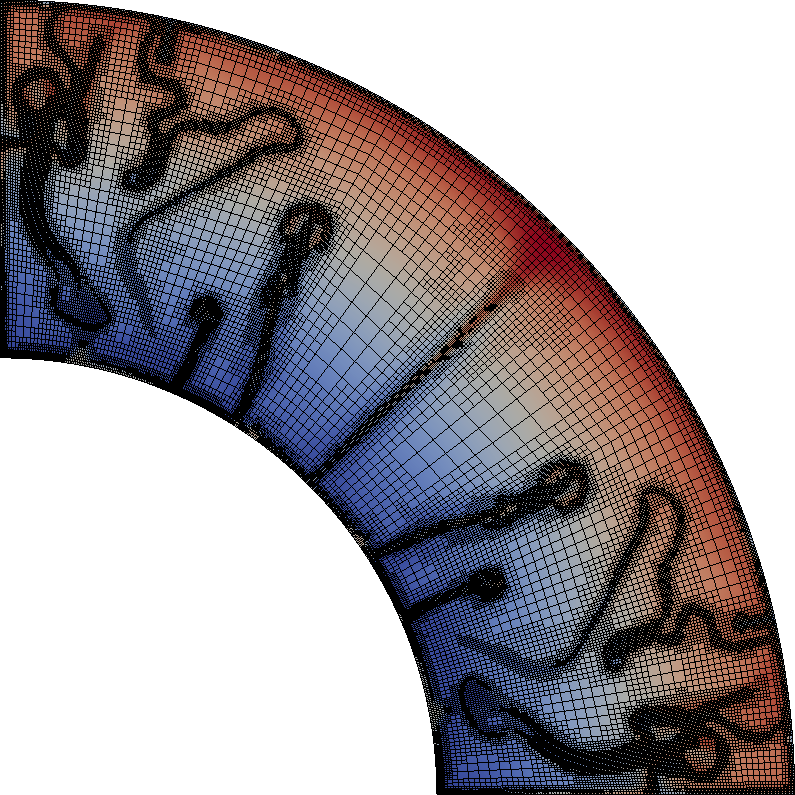
\includegraphics[width=0.6\textwidth]{mesh-2d.png}

  \vfill

  {\huge \aspect{}}
  \\[.3cm]
  {\Large
    Advanced Solver for Problems in Earth's
    ConvecTion}
  \\[.5cm]
  {\large Preview release, version 0.8\\
   (generated from subversion: $Revision$)}
  \\[1cm]
  {\large
    Wolfgang Bangerth\\
    Timo Heister\\[24pt]
  }
\end{centering}
{\parindent0pt
 \large
    with contributions by:\\
    Markus B{\"u}rg,
    Juliane Dannberg,
    Ren{\'e} Ga{\ss}m{\"o}ller,
    Thomas Geenen,
    Eric Heien,
    Martin Kronbichler
}



\pagebreak

\tableofcontents

\pagebreak

\section{Introduction}

\aspect{} --- short for Advanced Solver for Problems in Earth's ConvecTion ---
is a code intended to solve the equations that describe thermally driven
convection with a focus on doing so in the context of convection in the earth
mantle. It is primarily developed by computational scientists at Texas A\&M
University based on the following principles:
\begin{itemize}
\item \textit{Usability and extensibility:} Simulating mantle convection is a
  difficult problem characterized not only by complicated and nonlinear
  material models but, more generally, by a lack of understanding which parts
  of a much more complicated model are really necessary to simulate the
  defining features of the problem. To name just a few examples:
  \begin{itemize}
  \item Mantle convection is often solved in a spherical shell geometry, but
    the earth is not a sphere -- its true shape on the longest lengthscales is
    dominated by polar oblateness, but deviations from spherical shape
    relevant to convection patterns may go down to the lengthscales of
    mountain belts, mid-ocean ridges or subduction trenches. Furthermore,
    processes outside the mantle like crustal depression during glaciations
    can change the geometry as well.
  \item Rocks in the mantle flow on long time scales, but on shorter time
    scales they behave more like a visco-elasto-plastic material as they break
    and as their crystalline structure heals again. The mathematical models
    discussed in Section~\ref{sec:models} can therefore only be
    approximations.
    \item If pressures are low and temperatures high enough, rocks melt,
      leading to all sorts of new and interesting behavior.
  \end{itemize}
  This uncertainty in what problem one actually wants to solve requires a code
  that is easy to extend by users to support the community in determining what
  the essential features of convection in the earth mantle are. Achieving this
  goal also opens up possibilities outside the original scope, such as the
  simulation of convection in exoplanets or the icy satellites of the gas
  giant planets in our solar system.

\item \textit{Modern numerical methods:} We build \aspect{} on numerical
  methods that are at the forefront of research in all areas -- adaptive mesh
  refinement, linear and nonlinear solvers, stabilization of
  transport-dominated processes. This implies complexity in our algorithms,
  but also guarantees highly accurate solutions while remaining efficient in
  the number of unknowns and with CPU and memory resources.

\item \textit{Parallelism:} Many convection processes of interest are
  characterized by small features in large domains -- for example, mantle
  plumes of a few tens of kilometers diameter in a mantle almost 3,000 km
  deep. Such problems can not be solved on a single computer but require
  dozens or hundreds of processors to work together. \aspect{} is designed
  from the start to support this level of parallelism.

\item \textit{Building on others' work:} Building a code that satisfies above
  criteria from scratch would likely require several 100,000 lines of
  code. This is outside what any one group can achieve on academic time
  scales. Fortunately, most of the functionality we need is already available
  in the form of widely used, actively maintained, and well tested and
  documented libraries, and we leverage these to make \aspect{} a much smaller
  and easier to understand system. Specifically, \aspect{} builds immediately
  on top of the \dealii{} library (see \url{http://www.dealii.org/}) for
  everything that has to do with finite elements, geometries, meshes, etc.;
  and, through \dealii{} on Trilinos (see \url{http://trilinos.sandia.gov/})
  for parallel linear algebra and on \pfrst{} (see
  \url{http://www.p4est.org/}) for parallel mesh handling.
\end{itemize}

Combining all of these aspects into one code makes for an interesting
challenge. We hope to have achieved our goal of providing a useful tool to the
geodynamics community and beyond!


\note{\aspect{} is a community project. As such, we encourage contributions
  from the community to improve this code over time. Natural candidates for
  such contributions are implementations of new plugins as discussed in
  Section~\ref{sec:plugins-concrete} since they are typically self-contained and do not
  require much knowledge of the details of the remaining code. Obviously,
  however, we also encourage contributions to the core functionality in any
  form! If you have something that might be of general interest, please
  contact us.}

\note{\aspect{} will only solve problems relevant to the community if we get
  feedback from the community on things that are missing or necessary for what
  you want to do. Let us know by personal email to the developers, or the
  mantle convection or \texttt{aspect-devel} mailing lists hosted at
  \url{http://geodynamics.org/cgi-bin/mailman/listinfo/aspect-devel}!}

\subsection{Referencing \aspect{}}

As with all scientific work, funding agencies have a reasonable expectation
that if we ask for continued funding for this work, we need to demonstrate
relevance. To this end, we ask that if you publish results that were obtained
to some part using \aspect{}, you cite the following, canonical reference for
this software:
\begin{lstlisting}[frame=single,language=tex]
@Article{KHB12,
  author = 	 {Martin Kronbichler and Timo Heister and Wolfgang Bangerth},
  title = 	 {High Accuracy Mantle Convection Simulation through Modern Numerical Methods},
  journal = 	 {Geophysics Journal International},
  year = 	 2012,
  volume = 	 191,
  pages = 	 {12--29}}
\end{lstlisting}


\subsection{Acknowledgments}

The development of \aspect{} has been funded
through a variety of grants to the authors. Most immediately, it has been
supported through the Computational Infrastructure in Geodynamics (CIG-II)
grant (National Science Foundation Award No. EAR-0949446, via The University
of California -- Davis) but the initial portions have also been supported
by the original CIG grant (National Science Foundation Award No. EAR-0426271,
via The California Institute of Technology). In addition, the libraries upon
which \aspect{} builds heavily have been supported through many other grants
that are equally gratefully acknowledged.


\section{Equations, models, coefficients}
\label{sec:models}

\subsection{Basic equations}
\label{sec:equations}

\aspect{} solves a system of equations in a $d=2$- or $d=3$-dimensional
domain $\Omega$ that describes the motion of a highly viscous fluid driven
by differences in the gravitational force due to a density that depends on
the temperature. In the following, we largely follow the exposition of this
material in Schubert, Turcotte and Olson \cite{STO01}.

Specifically, we consider the following set of equations for velocity $\mathbf
u$, pressure $p$ and temperature $T$, as well as a set of advected quantities
$c_i$ that we call \textit{compositional fields}:
\marginpar{To be finished}
\marginpar{Wouldn't the last term need to have a minus sign? drho/dT
  is negative...}
\begin{align}
  \label{eq:stokes-1}
  -\nabla \cdot \left[2\eta \left(\varepsilon(\mathbf u)
                                  - \frac{1}{3}(\nabla \cdot \mathbf u)\mathbf 1\right)
                \right] + \nabla p &=
  \rho \mathbf g
  & \qquad
  & \textrm{in $\Omega$},
  \\
  \label{eq:stokes-2}
  \nabla \cdot (\rho \mathbf u) &= 0
  & \qquad
  & \textrm{in $\Omega$},
  \\
  \label{eq:temperature}
  \rho C_p \left(\frac{\partial T}{\partial t} + \mathbf u\cdot\nabla T\right)
  - \nabla\cdot k\nabla T
  &=
  \rho H
  \notag
  \\
  &\quad
  +
  2\eta
  \left(\varepsilon(\mathbf u) - \frac{1}{3}(\nabla \cdot \mathbf u)\mathbf 1\right)
  :
  \left(\varepsilon(\mathbf u) - \frac{1}{3}(\nabla \cdot \mathbf u)\mathbf 1\right)
  \\
  &\quad
  +\frac{\partial \rho}{\partial T} T \mathbf u \cdot \mathbf g
  & \quad
  & \textrm{in $\Omega$},
  \notag
  \\
  \label{eq:compositional}
  \frac{\partial c_i}{\partial t} + \mathbf u\cdot\nabla T
  &=
  0
  & \quad
  & \textrm{in $\Omega$},
  i=1\ldots C
\end{align}
where $\varepsilon(\mathbf u) = \frac{1}{2}(\nabla \mathbf u + \nabla\mathbf
u^T)$ is the symmetric gradient of the velocity (often called the
\textit{strain rate}).

In this set of equations, \eqref{eq:stokes-1} and \eqref{eq:stokes-2}
represent the compressible Stokes equations in which $\mathbf u=\mathbf
u(\mathbf x,t)$ is the velocity field and $p=p(\mathbf x,t)$ the pressure
field. Both fields depend on space $\mathbf x$ and time $t$. Fluid flow is
driven by the gravity force that acts on the fluid and that is proportional to
both the density of the fluid and the strength of the gravitational pull.

Coupled to this Stokes system is equation \eqref{eq:temperature} for the
temperature field $T=T(\mathbf x,t)$ that contains heat conduction terms as
well as advection with the flow velocity $\mathbf u$. The right hand side
terms of this equation correspond to
\begin{itemize}
\item internal heat production for example due to radioactive
  decay;
\item friction heating;
\item adiabatic compression of material; as written, this term assumes that
  the the overall pressure is dominated by the hydrostatic pressure, in which
  case the variation of the total pressure can be expressed by gravity and
  density.
\end{itemize}
The equations \aspect{} currently solves do not include phase change terms,
see Section~\ref{sec:future}.

The final set equations, \eqref{eq:compositional}, describes the motion of
a set of advected quantities $c_i(\mathbf x,t),i=1\ldots C$. We call these
\textit{compositional fields} because we think of them as spatially and
temporally varying concentrations of different elements, minerals, or other
constituents of the composition of the material that convects. As such, these
fields participate actively in determining the values of the various
coefficients of these equations. On the other hand, \aspect{} also allows the
definition of material models that are independent of these compositional
fields, making them passively advected quantities. Several of the cookbooks in
Section~\ref{sec:cookbooks} consider compositional fields in this way, i.e.,
essentially as tracer quantities that only keep track of where material came
from.

These equations are
augmented by boundary conditions that can either be of Dirichlet-, Neumann, or
tangential type on subsets of the boundary $\Gamma=\partial\Omega$:
\begin{align}
  \mathbf u &= 0 & \qquad &\textrm{on $\Gamma_{0,\mathbf u}$},
  \\
  \mathbf n \cdot \mathbf u &= 0 & \qquad &\textrm{on $\Gamma_{\parallel,\mathbf u}$},
  \\
  T &= T_{\text{prescribed}}
   & \qquad &\textrm{on $\Gamma_{D,T}$},
  \\
  \mathbf n \cdot k\nabla T &= 0
   & \qquad &\textrm{on $\Gamma_{N,T}$}.
  \\
  c_i &= 0
   & \qquad &\textrm{on $\Gamma_\textit{in}=\{\mathbf x: \mathbf
   u\cdot\mathbf n<0\}$}.
\end{align}
Here,
$\Gamma_{0,\mathbf u}$ corresponds to parts of the boundary on which the
velocity is fixed to be zero,
$\Gamma_{\parallel,\mathbf u}$ to parts of the boundary on which the
velocity may be nonzero but must be parallel to the boundary,
$\Gamma_{D,T}$ to places where the temperature is prescribed (for example at
the inner and outer boundaries of the earth mantle), and finally
$\Gamma_{N,T}$ to places where the temperature is unknown but the heat flux
across the boundary is zero (for example on symmetry surfaces if only a part
of the shell that constitutes the domain the Earth mantle occupies is
simulated). We require that one of these boundary conditions hold at each
point for both velocity and temperature, i.e.,
$\Gamma_{0,\mathbf u}\cup\Gamma_{\parallel,\mathbf u}=\Gamma$ and
$\Gamma_{D,T}\cup\Gamma_{N,T}=\Gamma$. No boundary conditions have to be posed
for the compositional fields at those parts of the boundary where flow is either
tangential to the boundary or points outward.

\aspect{} solves these equations in essentially the form stated. In
particular, the form given in \eqref{eq:stokes-1} implies that the pressure
$p$ we compute is in fact the \textit{total pressure}, i.e., the sum of
hydrostatic pressure and dynamic pressure (however, see
Section~\ref{sec:pressure-static-dyn} for more information on this, as well as
the extensive discussion of this issue in \cite{KHB12}).
Consequently, it allows the direct use of this pressure when looking up
pressure dependent material parameters.


\subsection{Coefficients}
\label{sec:coefficients}

The equations above contain a significant number of coefficients that we will
discuss in the following. In the most general form, many of these coefficients
depend nonlinearly on the solution variables pressure $p$, temperature $T$
and, in the case of the viscosity, on the strain rate $\varepsilon(\mathbf
u)$. If compositional fields $\mathfrak c=\{c_1,\ldots,c_C\}$ are present (i.e.,
if $C>0$), coefficients may also depend on them. Alternatively, they may be
parameterized as a function
of the spatial variable $\mathbf x$. \aspect{} allows both kinds of
parameterizations.

\note{One of the next versions of \aspect{} will actually iterate out
  nonlinearities in the material description. However, in the current version,
  we simply evaluate all nonlinear dependence of coefficients at the solution
  variables from the previous time step or a solution suitably extrapolated from
  the previous time steps.}

Note that below we will discuss examples of the dependence of coefficients on
other quantities; which dependence is actually implemented in the code is a
different matter. As we will discuss in Section~\ref{sec:parameters} and
\ref{sec:extending}, some versions of these models are already implemented and
can be selected from the input parameter file; others are easy to add to
\aspect{} by providing self-contained descriptions of a set of coefficients
that the rest of the code can then use without a need for further
modifications.

Concretely, we consider the following coefficients and dependencies:
\begin{itemize}
\item \textit{The viscosity $\eta=\eta(p,T,\varepsilon(\mathbf u),\mathfrak
c,\mathbf x)$:} Units $\textrm{Pa}\cdot \textrm{s} =
  \textrm{kg}\frac{1}{\textrm{m}\cdot\textrm{s}}$.

  The viscosity is the proportionality factor that relates total forces
  (external gravity minus pressure gradients) and fluid velocities $\mathbf
  u$. The simplest models assume that $\eta$ is constant, with the constant
  often chosen to be on the order of $10^{21} \textrm{Pa}\;\textrm{s}$.

  More complex (and more realistic) models assume that the viscosity depends
  on pressure, temperature and strain rate. Since this dependence is often
  difficult to quantify, one modeling approach is to make $\eta$ spatially
  dependent.

\item \textit{The density $\rho=\rho(p,T,\mathfrak c,\mathbf x)$:} Units
  $\frac{\textrm{kg}}{\textrm{m}^3}$.

  In general, the density depends on pressure and temperature, both through
  pressure compression, thermal expansion, and phase changes the material may
  undergo as it moves through the pressure-temperature phase diagram.

  The simplest parameterization for the density is to assume a linear
  dependence on temperature, yielding the form
  $\rho(T)=\rho_{\text{ref}}[1-\beta (T-T_{\text{ref}})]$ where
  $\rho_{\text{ref}}$ is the reference density at temperature $T_{\text{ref}}$
  and $\beta$ is the linear thermal expansion coefficient. For the earth
  mantle, typical values for this parameterization would be
  $\rho_{\text{ref}}=3300\frac{\textrm{kg}}{\textrm{m}^3}$,
  $T_{\text{ref}}=293 \textrm{K}$, $\beta=2\cdot 10^{-5}
  \frac{1}{\mathrm{K}}$.

\item \textit{The gravity vector $\mathbf g=\mathbf g(\mathbf x)$:} Units
  $\frac{\textrm{m}}{\textrm{s}^2}$.

  Simple models assume a radially inward gravity vector of constant magnitude
  (e.g., the surface gravity of Earth, $9.81 \frac{\textrm{m}}{\textrm{s}^2}$),
  or one that can be computed analytically assuming a homogenous mantle
  density.

  A physically self-consistent model would compute the gravity vector as
  $\mathbf g = -\nabla \varphi$ with a gravity potential $\varphi$ that
  satisfies $-\Delta\varphi=4\pi G\rho$ with the density $\rho$ from above and
  $G$ the universal constant of gravity. This would provide a gravity vector
  that changes as a function of time. Such a model is not currently
  implemented.

\item \textit{The specific heat capacity $C_p=C_p(p,T,\mathfrak c,\mathbf x)$:}
Units $\frac{\textrm{J}}{\textrm{kg}\cdot\textrm{K}} =
  \frac{\textrm{m}^2}{\textrm{s}^2\cdot\textrm{K}}$.

  The specific heat capacity denotes the amount of energy needed to increase
  the temperature of one kilogram of material by one degree. Wikipedia lists a
  value of 790 $\frac{\textrm{J}}{\textrm{kg}\cdot\textrm{K}}$ for granite%
  \footnote{See \url{http://en.wikipedia.org/wiki/Specific_heat}.}
  For the earth mantle, a value of 1250
  $\frac{\textrm{J}}{\textrm{kg}\cdot\textrm{K}}$ is within the range
  suggested by the literature.


\item \textit{The thermal conductivity $k=k(p,T,\mathfrak c,\mathbf x)$:} Units
  $\frac{\textrm{W}}{\textrm{m}\cdot\textrm{K}}=\frac{\textrm{kg}\cdot\textrm{m}}{\textrm{s}^3\cdot\textrm{K}}$.

  The thermal conductivity denotes the amount of thermal energy flowing
  through a unit area for a given temperature gradient. It depends on the
  material and as such will from a physical perspective depend on pressure and
  temperature due to phase changes of the material as well as through
  different mechanisms for heat transport (see, for example, the partial
  transparency of perovskite, the most abundant
  material in the earth mantle, at pressures above around 120 GPa
  \cite{BRVMFG04}).

  As a rule of thumb for its
  order of magnitude, wikipedia quotes values of
  $1.83$--$2.90\frac{\textrm{W}}{\textrm{m}\cdot\textrm{K}}$ for sandstone and
  $1.73$--$3.98\frac{\textrm{W}}{\textrm{m}\cdot\textrm{K}}$ for granite.%
  \footnote{See \url{http://en.wikipedia.org/wiki/Thermal_conductivity} and
    \url{http://en.wikipedia.org/wiki/List_of_thermal_conductivities}.} The
  values in the mantle are almost certainly higher than this though probably
  not by much. The exact value is not really all that important: heat
  transport through convection is several orders of magnitude more important
  than through thermal conduction.

\item \textit{The intrinsic specific heat production $H=H(\mathbf x)$:} Units
  $\frac{\textrm{W}}{\textrm{kg}}=\frac{\textrm{m}^2}{\textrm{s}^3}$.

  This term denotes the intrinsic heating of the material, for example due to
  the decay of radioactive material. As such, it depends not on pressure or
  temperature, but may depend on the location due to different chemical
  composition of material in the earth mantle. The literature suggests a value
  of $\gamma=7.4\cdot 10^{-12}\frac{\textrm{W}}{\textrm{kg}}$.
\end{itemize}


\subsection{Dimensional or non-dimensionalized equations?}
\label{sec:non-dimensional}

Equations \eqref{eq:stokes-1}--\eqref{eq:temperature} are stated in the
physically correct form. One would usually interpret them in a way that the
various coefficients such as the viscosity, density and thermal conductivity
$\eta,\rho,\kappa$ are given in their correct physical units, typically
expressed in a system such as the meter, kilogram, second (MKS) system that is
part of the \href{http://en.wikipedia.org/wiki/SI}{SI} system.
This is certainly how we envision \aspect{} to be used: with geometries,
material models, boundary conditions and initial values to be given in their correct
physical units. As a consequence, when \aspect{} prints information about the
simulation onto the screen, it typically does so by using a postfix such as
\texttt{m/s} to indicate a velocity or \texttt{W/m\^{}2} to indicate a heat
flux.

\note{For convenience, output quantities are sometimes provided
  in units meters per \textit{year} instead of meters per \textit{second}
  (velocities) or in \textit{years} instead of \textit{seconds} (the current
  time, the time step size); this
  conversion happens at the time output is generated, and is not part of the
  solution process. Whether this conversion should happen is determined by the
  flag ``\texttt{Use years in output instead of seconds}'' in the input file,
\index[prmindex]{Use years in output instead of seconds}
\index[prmindexfull]{Use years in output instead of seconds}
  see Section~\ref{parameters:global}. Obviously, this conversion from seconds
  to years only makes sense if the model is described in physical units rather
  than in non-dimensionalized form, see below.}

That said, in reality, \aspect{} has no preferred system of
units as long as every material constant, geometry, time, etc., are all
expressed in the same system. In other words, it is entirely legitimate to
implement geometry and material models in which the dimension of the domain is
one, density and viscosity are one, and the density variation as a function of
temperature is scaled by the Rayleigh number -- i.e., to use the usual
non-dimensionalization of the Boussinesq equations. Some of the cookbooks in
Section~\ref{sec:cookbooks} use this non-dimensional form; for example,
the simplest cookbook in Section~\ref{sec:cookbooks-simple-box} as well as
the SolCx, SolKz and inclusion benchmarks in Sections~\ref{sec:benchmark-solcx},
are such cases. Whenever this is the case, output showing units \texttt{m/s} or
\texttt{W/m\^{}2} clearly no longer have a literal meaning. Rather, the unit postfix must in this case simply
be interpreted to mean that the number that precedes the first is a velocity and
a heat flux in the second case.

In other words, whether a computation uses physical or non-dimensional units
really depends on the geometry, material, initial and boundary condition
description of the particular case under consideration -- \aspect{} will simply
use whatever it is given. Whether one or the other is the more appropriate
description is a decision we purposefully leave to the user. There are of
course good reasons to use non-dimensional descriptions of realistic problems,
rather than to use the original form in which all coefficients remain in their
physical units. On the other hand, there are also downsides:
\begin{itemize}
  \item Non-dimensional descriptions, such as when using the
  \href{http://en.wikipedia.org/wiki/Rayleigh_number}{Rayleigh} number to
  indicate the relative strength of convective to diffusive thermal transport,
  have the advantage that they allow to reduce a system to its essence. For
  example, it is clear that we get the same behavior if one increases both the
  viscosity and the thermal expansion coefficient by a factor of two because the
  resulting Rayleigh number; similarly, if we were to increase the size of the
  domain by 2 and thermal diffusion coefficient by a factor of 8. In both of
  these cases, the non-dimensional equations are exactly the same. On the other
  hand, the equations in their physical unit form are different and one may not
  see that the result of this variations in coefficients will be exactly the
  same as before. Using non-dimensional variables therefore reduces the space of
  independent parameters one may have to consider when doing parameter studies.

  \item From a practical perspective, equations
  \eqref{eq:stokes-1}--\eqref{eq:temperature} are often ill-conditioned in
  their original form: the two sides of each equation have physical units
  different from those of the other equations, and their numerical values are
  often vastly different.%
  \footnote{To illustrate this, consider convection in the Earth as a
  back-of-the-envelope example.
  With the length scale of the mantle $L=3\cdot 10^6\;m$, viscosity
  $\eta=10^{24} \; kg/m/s$, density $\rho=3\cdot 10^3 \; kg/m^3$ and a typical
  velocity of $U=0.1\;m/year=3\cdot 10^{-9}\; m/s$, we get that the friction
  term in \eqref{eq:stokes-1} has size $\eta U/L^2 \approx 3\cdot 10^2 \;
  kg/m/s^3$. On the other hand, the term $\nabla\cdot(\rho u)$ in the
  continuity equation \eqref{eq:stokes-2} has size $\rho U/L\approx 3\cdot
  10^{-12} \; kg/s/m^3$. In other words, their \textit{numerical values} are 14
  orders of magnitude apart.}
  Of course, these values can not be compared: they have different physical
  units, and the ratios between these values depends on whether we choose to
  measure lengths in meters or kilometers, for example. Nevertheless, when
  implementing these equations in software, at one point or another, we have to
  work with numbers and at this point the physical units are lost. If one does
  not take care at this point, it is easy to get software in which all accuracy
  is lost due to round-off errors. On the other hand, non-dimensionalization
  typically avoids this since it normalizes all quantities so that values that
  appear in computations are typically on the order of one.

  \item On the downside, the numbers non-dimensionalized equations produce are
  not immediately comparable to ones we know from physical experiments. This is
  of little concern if all we have to do is convert every output number of our
  program back to physical units. On the other hand, it is more difficult and a
  source of many errors if this has to be done inside the program, for example,
  when looking up the viscosity as a pressure-, temperature- and
  strain-rate-dependent function: one first has to convert pressure,
  temperature and strain rate from non-dimensional to physical units, look up
  the corresponding viscosity in a table, and then convert the viscosity back to
  non-dimensional quantities. Getting this right at every one of the dozens or
  hundreds of places inside a program, using the correct (but distinct)
  conversion factors for each of these quantities, is a challenge and a source
  of errors.

  \item From a mathematical viewpoint, it is typically clear how an equation
  needs to be non-dimensionalized if all coefficients are constant. However, how
  is one to normalize the equations if, as is the case in the earth mantle, the
  viscosity varies by several orders of magnitude? In cases like these, one has
  to choose a reference viscosity, density, etc. While the resulting
  non-dimensionalization retains the universality of parameters in the
  equations, as discussed above, it is not entirely clear that this would also
  retain the numerical stability if the reference values are poorly chosen.
\end{itemize}

As a consequency of such considerations, most codes in the past have used
non-dimensionalized models. This was aided by the fact that until recently and
with notable exceptions, many models had constant coefficients and the
difficulties associated with variable coefficients were not a concern. On the
other hand, our goal with \aspect{} is for it to be a code that solves realistic
problems using complex models and that is easy to use. Thus, we allow users to
input models in physical or non-dimensional units, at their discretion. We
believe that this makes the description of realistic models simpler. On
the other hand, ensuring numerical stability is not something users should have
to be concerned about, and is taken care of in the implementation of \aspect{}'s
core (see the corresponding section in \cite{KHB12}).



\subsection{Static or dynamic pressure?}
\label{sec:pressure-static-dyn}

One could reformulate equation \eqref{eq:stokes-1} somewhat. To this end, let us
say that we would want to represent the pressure $p$ as the sum of two parts
that we will call static and dynamic, $p=p_s+p_d$. If we assume that $p_s$ is
already given, then we can replace \eqref{eq:stokes-1} by
\begin{gather*}
  -\nabla \cdot 2\eta
  \nabla \mathbf u + \nabla p_d =
  \rho\mathbf g - \nabla p_s.
\end{gather*}
One typically chooses $p_s$ as the pressure one would get if the whole medium
were at rest -- i.e., as the hydrostatic pressure. This pressure can be
computed noting that \eqref{eq:stokes-1} reduces to
\begin{gather*}
  \nabla p_s = \rho(p_s,T_s,\mathbf x)\mathbf g
\end{gather*}
in the absence of any motion where $T_s$ is some static temperature field (see
also Section~\ref{sec:adiabatic}). This, our rewritten version of
\eqref{eq:stokes-1} would look like this:
\begin{gather*}
  -\nabla \cdot 2\eta
  \nabla \mathbf u + \nabla p_d =
  \left[\rho(p,T,\mathbf x)-\rho(p_s,T_s,\mathbf x)\right]\mathbf g.
\end{gather*}
In this
formulation, it is clear that the quantity that drives the fluid flow is in
fact the \textit{buoyancy} caused by the \textit{variation} of densities,
not the density itself.

This reformulation has a number of advantages and disadvantages:
\begin{itemize}
\item One can notice that in many realistic cases, the dynamic component $p_d$
  of the pressure is orders of magnitude smaller than the static component
  $p_s$. For example, in the earth, the two are separated by around 6 orders
  of magnitude at the bottom of the earth mantle. Consequently, if one wants
  to solve the linear system that arises from discretization of the original
  equations, one has to solve it a significant degree of accuracy (6--7
  digits) to get the dynamic part of the pressure correct to even one
  digit. This entails a very significant numerical effort, and one that is not
  necessary if we can split the pressure in a way so that the pre-computed
  static pressure $p_s$ (or, rather, the density using the static pressure and
  temperature from which $p_s$ results) absorbs the dominant part and one only
  has to compute the remaining, dynamic pressure to 2 or 3 digits of accuracy,
  rather than the corresponding 7--8 for the total pressure.

\item On the other hand, the pressure $p_d$ one computes this way is not immediately
  comparable to quantities that we use to look up pressure-dependent
  quantities such as the density. Rather, one needs to first find the static
  pressure as well (see Section~\ref{sec:adiabatic}) and add the two together
  before they can be used to look up material properties or to compare them with
  experimental results. Consequently, if the pressure a program outputs
  (either for visualization, or in the internal interfaces to parts of the
  code where users can implement pressure- and temperature-dependent material
  properties) is only the dynamic component, then all of the consumers of this
  information need to convert it into the total pressure when comparing with
  physical experiments. Since any code implementing realistic material models
  has a great many of these places, there is a large potential for inadvertant
  errors and bugs.

\item Finally, the definition of a reference density $\rho(p_s,T_s,\mathbf x)$
  derived from static pressures and temperatures
  is only simple if we have incompressible models and under the assumption
  that the temperature-induced density variations are small compared to the
  overall density. In this case, we can choose $\rho(p_s,T_s,\mathbf
  x)=\rho_0$ with a constant reference density $\rho_0$. On the other hand,
  for more complicated models, it is not a priori
  clear which density to choose since we first need to compute static
  pressures and temperatures -- quantities that satisfy equations that
  introduce boundary layers, may include phase changes releasing latent heat,
  and where the density may have discontinuities at certain depths, see
  Section~\ref{sec:adiabatic}.

  Thus, if we compute adiabatic pressures and
  temperatures $\bar p_s,\bar T_s$ under the assumption of a thermal boundary layer
  worth 900 Kelvin at the top, and we get a corresponding density profile
  $\bar\rho=\rho(\bar p_s,\bar T_s, \mathbf x)$, but after running for a few
  million years the temperature turns out to be so that the top boundary layer
  has a jump of only 800 Kelvin with corresponding adiabatic pressures and
  temperatures $\hat p_s,\hat T_s$, then a more appropriate density profile
  would be $\hat\rho=\rho(\hat p_s,\hat T_s, \mathbf x)$.

  The problem is that it may well be that the erroneously computed density
  profile $\hat \rho$ does \textit{not} lead to a separation where
  $|p_d|\ll|p_s|$ because, especially if the material undergoes phase changes,
  there will be entire areas of the computational domain in which $|\rho-\hat
  \rho_s|\ll |\rho|$ but $|\rho-\bar
  \rho_s|\not\ll |\rho|$. Consequently the benefits of lesser requirements on the
  iterative linear solver would not be realized.
\end{itemize}

We do note that most of the codes available today and that we are aware of
split the pressure into static and dynamic parts nevertheless, either
internally or require the user to specify the density profile as the
difference between the true and the hydrostatic density. This may, in part, be
due to the fact that historically most codes where written to solve problems
in which the medium was considered incompressible, i.e., where the definition
of a static density was simple.

On the other hand, we intend \aspect{} to be a code that can solve more
general models for which this definition is not as simple. As a consequence, we
have chosen to solve the equations as stated originally -- i.e., we solve for
the \textit{full} pressure rather than just its \textit{dynamic} component. With
most traditional methods, this would lead to a catastrophic loss of accuracy in the
dynamic pressure since it is many orders of magnitude smaller than the total
pressure at the bottom of the earth mantle. We avoid this problem in \aspect{}
by using a cleverly chosen iterative solver that ensures that the full pressure
we compute is accurate enough so that the dynamic pressure can be extracted from
it with the same accuracy one would get if one were to solve for only the
dynamic component. The methods that ensure this are described in detail in
\cite{KHB12} and in particular in the appendix of that paper.


\subsection{Pressure normalization}
\label{sec:pressure}

The equations described above, \eqref{eq:stokes-1}--\eqref{eq:temperature},
only determine the pressure $p$ up to an additive constant. On the other hand,
since the pressure appears in the definition of many of the coefficients, we
need a pressure that has some sort of \textit{absolute} definition. A
physically useful definition would be to normalize the pressure in such a way
that the average pressure along the ``surface'' has a prescribed value where
the geometry description (see Section~\ref{sec:geometry-models}) has to
determine which part of the boundary of the domain is the ``surface'' (we call
a part of the boundary the ``surface'' if its depth is ``close to zero'').

Typically, one will choose this average pressure to be zero, but there is a
parameter ``\texttt{Surface pressure}''
\index[prmindex]{Surface pressure}
\index[prmindexfull]{Surface pressure}
in the input file (see Section~\ref{parameters:global}) to set it to
a different value. One may want to do that, for example, if one wants to
simulate the earth mantle without the overlying lithosphere. In that case, the
``surface'' would be the interface between mantle and lithosphere, and the
average pressure at the surface to which the solution of the equations will be
normalized should in this case be the hydrostatic pressure at the bottom of
the lithosphere.

An alternative is to normalize the pressure in such a way that the
\textit{average} pressure throughout the domain is zero or some constant
value. This is not a useful approach for most geodynamics applications but is
common in benchmarks for which analytic solutions are available. Which kind of
normalization is chosen is determined by the ``\texttt{Pressure
  normalization}'' flag in the input file,
\index[prmindex]{Pressure normalization}
\index[prmindexfull]{Pressure normalization}
see Section~\ref{parameters:global}.


\subsection{Initial conditions and the adiabatic pressure/temperature}
\label{sec:adiabatic}

Equations \eqref{eq:stokes-1}--\eqref{eq:temperature} require us to
pose initial conditions for the temperature, and this is done by
selecting one of the existing models for initial conditions in the
input parameter file, see
Section~\ref{parameters:Initial_20conditions}. The equations
themselves do not require that initial conditions are specified for
the velocity and pressure variables (since there are no time
derivatives on these variables in the model).

Nevertheless, a nonlinear solver will have difficulty converging to
the correct solution if we start with a completely unphysical pressure
for models in which coefficients such as density $\rho$ and viscosity
$\eta$ depend on the pressure and temperature. To this end, \aspect{} computes
pressure and temperature fields $p_{\textrm{ad}}(z),
T_{\textrm{ad}}(z)$ that satisfy adiabatic conditions:
\begin{align}
  \rho C_p \frac{\textrm{d}}{\textrm{d}z} T_{\textrm{ad}}(z)
  &=
  \frac{\partial\rho}{\partial T} T_{\textrm{ad}}(z) g_z,
\\
  \frac{\textrm{d}}{\textrm{d}z} p_{\textrm{ad}}(z)
  &=
  \rho g_z,
\end{align}
where strictly speaking $g_z$ is the magnitude of the vertical
component of the gravity vector field, but in practice we take the
magnitude of the entire gravity vector.

These equations can be integrated numerically starting at $z=0$, using
the depth dependent gravity field and values of the coefficients
$\rho=\rho(p,T,z), C_p=C_p(p,T,z)$. As starting conditions at $z=0$ we
choose a pressure $p_{\textrm{ad}}(0)$ equal to the average surface
pressure (often chosen to be zero, see Section~\ref{sec:pressure}),
and an adiabatic surface temperature $T_{\textrm{ad}}(0)$ that is
\index[prmindex]{Adiabatic surface temperature}
\index[prmindexfull]{Adiabatic surface temperature}
also selected in the input parameter file.

\note{The adiabatic surface temperature is often chosen significantly
  higher than the actual surface temperature. For example, on earth,
  the actual surface temperature is on the order of 290 K, whereas a
  reasonable adiabatic surface temperature is maybe 1200 K. The reason
  is that the bulk of the mantle is more or less in thermal equilibrium
  with a thermal profile that corresponds to the latter temperature,
  whereas the very low actual surface temperature and the very high
  bottom temperature at the core-mantle boundary simply induce a
  thermal boundary layer. Since the temperature and pressure profile
  we compute using the equations above are simply meant to be good
  starting points for nonlinear solvers, it is important to choose
  this profile in such a way that it covers most of the mantle well;
  choosing an adiabatic surface temperature of 290 K would yield a
  temperature and pressure profile that is wrong almost throughout the
  entire mantle.}



\subsection{Numerical methods}

There is no shortage in the literature for methods to solve the equations
outlined above. The methods used by \aspect{} use the following,
interconnected set of strategies in the implementation of numerical
algorithms:
\begin{itemize}
\item \textit{Mesh adaptation:} Mantle convection problems are characterized
  by widely disparate length scales (from plate boundaries on the order of
  kilometers or even smaller, to the scale of the entire earth). Uniform
  meshes can not resolve the smallest length scale without an intractable
  number of unknowns.  Fully adaptive meshes allow resolving local features of
  the flow field without the need to refine the mesh globally. Since the
  location of plumes that require high resolution change and move with time,
  meshes also need to be adapted every few time steps.
\item \textit{Accurate discretizations:} The Boussinesq problem upon which
  most models for the earth mantle are based
  has a number of intricacies that make the choice of discretization
  non-trivial. In particular, the finite elements chosen for velocity and
  pressure need to satisfy the usual compatibility condition for saddle point
  problems. This can be worked around using pressure stabilization schemes for
  low-order discretizations, but high-order methods can yield better accuracy
  with fewer unknowns and offer more reliability. Equally important is the choice of
  a stabilization method for the highly advection-dominated temperature
  equation. \aspect{} uses a nonlinear artificial diffusion method for the latter.
\item \textit{Efficient linear solvers:} The major obstacle in solving the
  Boussinesq system is the saddle-point nature of the Stokes equations. Simple
  linear solvers and preconditioners can not efficiently solve this system in
  the presence of strong heterogeneities or when the size of the system
  becomes very large. \aspect{} uses an efficient solution strategy based on a
  block triangular preconditioner utilizing an algebraic multigrid that
  provides optimal complexity even up to problems with hundreds of millions of
  unknowns.
\item \textit{Parallelization of all of the steps above:} Global mantle convection
  problems frequently require extremely large numbers of unknowns for
  adequate resolution in three dimensional simulations. The only realistic way to solve such problems lies in
  parallelizing computations over hundreds or thousands of processors. This is
  made more complicated by the use of dynamically changing meshes, and it
  needs to take into account that we want to retain the optimal complexity of
  linear solvers and all other operations in the program.
\item \textit{Modularity of the code:} A code that implements all of these
  methods from \textit{scratch} will be unwieldy, unreadable and unusable as a community
  resource. To avoid this, we build our implementation on widely used and well
  tested libraries that can provide researchers interested in extending it
  with the support of a large user community. Specifically, we use the
  \dealii{} library \cite{BHK07,BK99m} for meshes, finite
  elements and everything discretization related; the \trilinos{} library
  \cite{trilinos,trilinos-web-page} for scalable and parallel linear algebra;
  and \pfrst{} \cite{p4est} for distributed, adaptive meshes. As a
  consequence, our code is freed of the mundane tasks of defining finite
  element shape functions or dealing with the data structures of linear algebra,
  can focus on the high-level description of what is supposed to happen, and
  remains relatively compact. The code will also
  automatically benefit from improvements to the underlying libraries with
  their much larger development communities. \aspect{} is extensively
  documented to enable other researchers to understand, test, use, and extend it.
\end{itemize}

Rather than detailing the various techniques upon which \aspect{} is built, we
refer to the paper by Kronbichler, Heister and Bangerth \cite{KHB12} that
gives a detailed description and rationale for the various building blocks.


\subsection{Simplifications of the basic equations}

There are two common variations to equations
\eqref{eq:stokes-1}--\eqref{eq:temperature} that are frequently used and that
make the system much simpler to solve and analyze: assuming that the fluid is
incompressible (the Boussinesq approximation) and a linear dependence of the
density on the temperature with constants that are otherwise independent of
the solution variables. These are
discussed in the following; \aspect{} has
run-time parameters that allow both of these simpler models to be used.

\subsubsection{The Boussinesq approximation: Incompressibility}
\label{sec:boussinesq}

The original Boussinesq approximation assumes that the density can be
considered constant in all occurrences in the equations with the exception of
the buoyancy term on the right hand side of \eqref{eq:stokes-1}. The primary
result of this assumption is that the continuity equation \eqref{eq:stokes-2}
will now read
\begin{gather*}
  \nabla \cdot \mathbf u = 0.
\end{gather*}
This makes the equations \textit{much} simpler to solve: First, because the
divergence operation in this equation is the transpose of the gradient of the
pressure in the momentum equation \eqref{eq:stokes-1}, making the system of
these two equations symmetric. And secondly, because the two equations are now
linear in pressure and velocity (assuming that the viscosity $\eta$ and the
density $\rho$ are considered fixed). In addition, one can drop all terms
involving $\nabla \cdot \mathbf u$ from the left hand side of the momentum
equation \eqref{eq:stokes-1} as well as from the shear heating term on the
right hand side of \eqref{eq:temperature}; while dropping these terms does not
affect the solution of the equations, it makes assembly of linear systems
faster. In addition, in the incompressible case, one needs to neglect the
adiabatic heating term $\frac{\partial \rho}{\partial T} T \mathbf u \cdot
\mathbf g$ on the right hand side of \eqref{eq:temperature}.

From a physical perspective, the assumption that the density is constant in
the continuity equation but variable in the momentum equation is of course
inconsistent. However, it is justified if the variation is small since the
momentum equation can be rewritten to read
\begin{gather*}
  -\nabla \cdot 2\eta \varepsilon(\mathbf u) + \nabla p_d =
  (\rho-\rho_0) \mathbf g,
\end{gather*}
where $p_d$ is the \textit{dynamic} pressure and $\rho_0$ is the constant
reference density. This makes it clear that the true driver of motion is in
fact the \textit{deviation} of the density from its background value, however
small this value is: the resulting velocities are simply proportional to the
density variation, not to the absolute magnitude of the density.

As such, the Boussinesq approximation can be justified. On the other hand,
given the real pressures and temperatures at the bottom of the earth mantle,
it is arguable whether the density can be considered to be almost
constant. Most realistic models predict that the density of mantle rocks
increases from somewhere around 3300 at the surface to over 5000 kilogram per
cubic meters at the core mantle boundary, due to the increasing lithostatic
pressure. While this appears to be a large variability, if the density changes
slowly with depth, this is not in itself an indication that the Boussinesq
approximation will be wrong. To this end, consider that the continuity
equation can be rewritten as $\frac 1\rho \nabla \cdot (\rho \mathbf u)=0$,
which we can multiply out to obtain
\begin{gather*}
  \nabla \cdot \mathbf u
  +
  \frac 1\rho \mathbf u \cdot \nabla \rho
  = 0.
\end{gather*}
The question whether the Boussinesq approximation is valid is then whether the
second term (the one omitted in the Boussinesq model) is small compared to the
first. To this end, consider that the velocity can change completely over length
scales of maybe 10 km, so that $\nabla \cdot\mathbf u \approx \|u\| /
10\text{km}$. On the other hand, given a smooth dependence of density on pressure,
the length scale for variation of the density is the entire earth mantle,
i.e., $\frac 1\rho \mathbf u \cdot \nabla\rho \approx \|u\| 0.5 / 3000 \text{km}$
(given a variation between minimal and maximal density of 0.5 times the
density itself). In other words, for a smooth variation, the contribution of
the compressibility to the continuity equation is very small. This may be
different, however, for models in which the density changes rather abruptly,
for example due to phase changes at mantle discontinuities.

In summary, models that use the approximation of incompressibility solve the
following set of equations instead of \eqref{eq:stokes-1}--\eqref{eq:temperature}:
\begin{align}
  \label{eq:stokes-1-boussinesq}
  -\nabla \cdot \left[2\eta \varepsilon(\mathbf u)
                \right] + \nabla p &=
  \rho \mathbf g
  & \qquad
  & \textrm{in $\Omega$},
  \\
  \label{eq:stokes-2-boussinesq}
  \nabla \cdot \mathbf u &= 0
  & \qquad
  & \textrm{in $\Omega$},
  \\
  \label{eq:temperature-boussinesq}
  \rho C_p \left(\frac{\partial T}{\partial t} + \mathbf u\cdot\nabla T\right)
  - \nabla\cdot k\nabla T
  &=
  \rho H
  +
  2\eta
  \varepsilon(\mathbf u)
  :
  \varepsilon(\mathbf u)
  & \quad
  & \textrm{in $\Omega$},
\end{align}
where the coefficients $\eta,\rho,\mathbf g,C_p$ may possible depend on the
solution variables.

\note{As we will see in Section~\ref{sec:extending}, it is easy to add new material
models to \aspect. Each model can decide whether it wants to use the
Boussinesq approximation or not. The description of the models in
Section~\ref{parameters:Material_20model} also gives an answer which of the
models already implemented uses the approximation or considers the material
sufficiently compressible to go with the fully compressible continuity equation.}


\subsubsection{Almost linear models}

A further simplification can be obtained if one assumes that all coefficients
with the exception of the density do not depend on the solution variables but
are, in fact, constant. In such models, one typically assumes that the density
satisfies a relationship of the form $\rho=\rho(T)=\rho_0(1-\beta(T-T_0))$
with a small thermal expansion coefficient $\beta$ and a reference density
$\rho_0$ that is attained at temperature $T_0$. Since the thermal expansion is
considered small, this naturally leads to the following variant of the Boussinesq
model discussed above:
\begin{align*}
  -\nabla \cdot \left[2\eta \varepsilon(\mathbf u)
                \right] + \nabla p &=
  \rho_0 (1-\beta (T-T_0)) \mathbf g
  & \qquad
  & \textrm{in $\Omega$},
  \\
  \nabla \cdot \mathbf u &= 0
  & \qquad
  & \textrm{in $\Omega$},
  \\
  \rho C_p \left(\frac{\partial T}{\partial t} + \mathbf u\cdot\nabla T\right)
  - \nabla\cdot k\nabla T
  &=
  \rho H
  +
  2\eta
  \varepsilon(\mathbf u)
  :
  \varepsilon(\mathbf u)
  & \quad
  & \textrm{in $\Omega$},
\end{align*}
If the gravitational acceleration $\mathbf g$ results from a gravity potential
$\varphi$ via $\mathbf g = -\nabla \varphi$, then one can rewrite the
equations above in the following, commonly used form:%
\footnote{Note, however, that \aspect{} does not solve the equations in the
  form given in
  \eqref{eq:stokes-1-boussinesq-linear}--\eqref{eq:temperature-boussinesq-linear}. Rather,
  it takes the original form with the real density, not the variation of
  the density. That said, you can use the formulation
  \eqref{eq:stokes-1-boussinesq-linear}--\eqref{eq:temperature-boussinesq-linear}
  by implementing a material model (see Section~\ref{sec:material-models}) in
  which the density in fact has the form $\rho(T)=\beta \rho_0 T$ even though
  this is not physical.}
\begin{align}
  \label{eq:stokes-1-boussinesq-linear}
  -\nabla \cdot \left[2\eta \varepsilon(\mathbf u)
                \right] + \nabla p_d &=
  -\beta\rho_0 T \mathbf g
  & \qquad
  & \textrm{in $\Omega$},
  \\
  \label{eq:stokes-2-boussinesq-linear}
  \nabla \cdot \mathbf u &= 0
  & \qquad
  & \textrm{in $\Omega$},
  \\
  \label{eq:temperature-boussinesq-linear}
  \rho C_p \left(\frac{\partial T}{\partial t} + \mathbf u\cdot\nabla T\right)
  - \nabla\cdot k\nabla T
  &=
  \rho H
  +
  2\eta
  \varepsilon(\mathbf u)
  :
  \varepsilon(\mathbf u)
  & \quad
  & \textrm{in $\Omega$},
\end{align}
where $p_d=p+\rho_0(1+\beta T_0)\varphi$ is the dynamic pressure, as opposed
to the total pressure $p=p_d+p_s$ that also includes the hydrastatic pressure
$p_s=-\rho_0(1+\beta T_0)\varphi$. Note that the right hand side forcing term
in \eqref{eq:stokes-1-boussinesq-linear} is now only the deviation of the
gravitational force from the force that would act if the material were at
temperature $T_0$.

Under the assumption that all other coefficients are constant, one then
arrives at equations in which the only nonlinear terms are the advection term,
$\mathbf u \cdot \nabla T$, and the shear friction, $2\eta\varepsilon(\mathbf
u):\varepsilon(\mathbf u)$, in the temperature equation
\eqref{eq:temperature-boussinesq-linear}. This facilitates the use of a
particular class of time stepping scheme in which one does not solve the whole
set of equations at once, iterating out nonlinearities as necessary, but
instead in each time step solves first the Stokes system with the previous
time step's temperature, and then uses the so-computed velocity to solve the
temperature equation. These kind of time stepping schemes are often referred
to as \textit{IMPES} methods (they originate in the porous media flow
community, where the acronym stands for \textit{Im}plicit \textit{P}ressure,
\textit{E}xplicit \textit{S}aturation). For details see \cite{KHB12}.

\note{In \aspect{} 0.1, using the IMPES scheme is the only available
  option. However, in later versions we will implement a fully nonlinear
  scheme that treats the equations as coupled, and one will be able to choose
  between the two variants using a run-time parameter.}


\section{Installation}

This is a brief explanation of how to install all the required software and
\aspect{} itself.

\subsection{Prerequisites}

\aspect{} builds on a few other libraries that are widely used in the
computational science area and that provide most of the lower-level
functionality such as finite element descriptions or parallel linear
algebra. Specifically, it builds on \dealii{} which in turn uses Trilinos and
\pfrst{}. These need to be installed first before you can compile and run
\aspect{}. All of these libraries can readily be installed in a user's home
directory, without the need to modify the overall system directories.

The following steps should guide you through the installation of these
prerequisites:
\begin{enumerate}
\item \textit{Trilinos:} Trilinos can be downloaded from
  \href{http://trilinos.sandia.gov/download/trilinos-10.12.html}{http://trilinos.sandia.gov/}. At
  the current time we recommend Trilinos Version 10.12.x.%
  \footnote{Other versions of Trilinos like 10.6.x
  and 10.8.x have bugs that make these versions unusable for our purpose. The
  \dealii{} ReadMe file provides a list of versions that are known to work
  without bugs with \dealii{}.} For installation instructions see
  \href{http://www.dealii.org/developer/readme-petsc-trilinos.html}{the deal.II README file on installing Trilinos and PETSc}. Note that you have
  to configure with MPI by using
\begin{verbatim}
 TPL_ENABLE_MPI:BOOL=ON
\end{verbatim}
  in the call to cmake. After that, run {\tt{make install}}.

\item \textit{\pfrst{}:} Download and install \pfrst{} as described in the
  \href{http://www.dealii.org/developer/external-libs/p4est.html}{deal.II
    p4est installation instructions}. This is done using the
  {\tt{p4est-setup.sh}}; do not use the \pfrst{} stand-alone installation
  instructions.

%\item  \textit{\dealii{}:}
%  The current version of \aspect{} requires features of \dealii{} that have
%  been developed after the 7.1 release. Since at the time of writing,
%  \dealii{} 7.2 has not yet appears, we currently require the development
%  version of \dealii{}, which can be obtained by running
%\begin{verbatim}
% svn checkout https://svn.dealii.org/trunk/deal.II
%\end{verbatim}
%  Once \dealii{} 7.2 is available, this will suffice as well.

\item \textit{\dealii{}:}
  The current version of \aspect{} requires \dealii{} version 7.3.0 or later.
  This version can be downloaded and installed from
  \url{https://code.google.com/p/dealii/downloads/list}.

  You may want to set the environment variable\footnote{For bash
    this would be adding the line {\tt{export DEAL\_DIR=/path/to/deal.ii/}} to
    the file {\tt{\~{}/.bashrc}}.}
{\tt{DEAL\_DIR}} to the directory where you checked out \dealii.

\item \textit{Configuring and compiling \dealii:} Now it is time to configure
  \dealii.
  To this end, follow the \dealii{}
  \href{http://www.dealii.org/developer/readme.html}{installation
    instructions}.
  Remember to point the {\tt{./configure}} script to the paths where
  you installed p4est and Trilinos and make sure you use MPI
  compilers. A typical command line would look like this:
\begin{verbatim}
 ./configure CXX=mpicxx --enable-mpi --disable-threads \
    --with-trilinos=/u/username/bin/trilinos-10.12.2 \
    --with-p4est=/u/username/bin/p4est-0.3.3.8
\end{verbatim}
  if the Trilinos and \pfrst{} packages have been installed in the
  subdirectory \texttt{/u/username/bin}.
  Make sure the configuration succeeds and detects the MPI compilers
  correctly. For more information see the documentation of \dealii.

  Now you are ready to compile \dealii{} by running {\tt{make all}}. If you
  have multiple processor cores, feel free to do {\tt{make all -jN}} where
  \texttt{N} is the number of processors in your machine to accelerate the
  process.

\item \textit{Testing your installation:} Test that your installation works
  by running the {\tt{step-32}} example that you can find in
  {\tt{\$DEAL\_DIR/examples/step-32}}. Compile by running {\tt{make}} and run
  with {\tt{mpirun -n 2 ./step-32}}.
\end{enumerate}


\subsection{Obtaining \aspect{} and initial configuration}

The development version of \aspect{} can be downloaded by executing the command
\begin{verbatim}
 svn checkout https://svn.aspect.dealii.org/trunk/aspect
\end{verbatim}
If {\tt{\$DEAL\_DIR}} points to your \dealii{} installation, there is no
further configuration that needs to be done, otherwise you need to edit
the {\tt{Makefile}} accordingly.


\subsection{Compiling \aspect{} and generating documentation}
\label{sec:compiling}

After downloading \aspect{} and having built the libraries it builds on, you
can compile it by typing
\begin{verbatim}
  make
\end{verbatim}
on the command line (or \texttt{make -jN} if you have multiple processors in
your machine, where \texttt{N} is the number of processors). This builds the
\aspect{} executable which will reside in
the \texttt{lib/} subdirectory and will be named \texttt{lib/aspect-2d} or
\texttt{lib/aspect-3d}, depending on the space dimension you compile for (see
Section~\ref{sec:2d-vs-3d} for more information on this). If you intend to
modify \aspect{} for your own experiments, you may want to also generate
documentation about the source code. This can be done using the command
\begin{verbatim}
  make doc
\end{verbatim}
which assumes that you have the \texttt{doxygen} documentation generation tool
installed. Most linux distributions have packages for \texttt{doxygen}. The
result will be the file \url{doc/doxygen/index.html} that is the starting
point for exploring the documentation.


\section{Running \aspect}
\label{sec:running}

\subsection{Overview}
\label{sec:running-overview}

After compiling \aspect{} as described above, you should have an executable
file in the \texttt{lib/} subdirectory. It can be called as follows:
\begin{verbatim}
  ./lib/aspect parameter-file.prm
\end{verbatim}
or, if you want to run the program in parallel, using something like
\begin{verbatim}
  mpirun -np 32 ./lib/aspect parameter-file.prm
\end{verbatim}
to run with 32 processors. In either case, the argument denotes the (path and)
name of a file that contains input parameters. When you download \aspect, you
should already have a sample input file in the top-level directory that gives
you an idea of the parameters that can be set. A full description of all
parameters is given in Section~\ref{sec:parameters}.

Running the program should produce output that will look something like this
(numbers will all be different, of course):
\begin{lstlisting}[frame=single,language=ksh]
Number of active cells: 1,536 (on 5 levels)
Number of degrees of freedom: 20,756 (12,738+1,649+6,369)

*** Timestep 0:  t=0 years

   Rebuilding Stokes preconditioner...
   Solving Stokes system... 30+3 iterations.
   Solving temperature system... 8 iterations.

Number of active cells: 2,379 (on 6 levels)
Number of degrees of freedom: 33,859 (20,786+2,680+10,393)

*** Timestep 0:  t=0 years

   Rebuilding Stokes preconditioner...
   Solving Stokes system... 30+4 iterations.
   Solving temperature system... 8 iterations.

   Postprocessing:
     Writing graphical output: output/solution-00000
     RMS, max velocity:        0.0946 cm/year, 0.183 cm/year
     Temperature min/avg/max:  300 K, 3007 K, 6300 K
     Inner/outer heat fluxes:  1.076e+05 W, 1.967e+05 W

*** Timestep 1:  t=1.99135e+07 years

   Solving Stokes system... 30+3 iterations.
   Solving temperature system... 8 iterations.

   Postprocessing:
     Writing graphical output: output/solution-00001
     RMS, max velocity:        0.104 cm/year, 0.217 cm/year
     Temperature min/avg/max:  300 K, 3008 K, 6300 K
     Inner/outer heat fluxes:  1.079e+05 W, 1.988e+05 W

*** Timestep 2:  t=3.98271e+07 years

   Solving Stokes system... 30+3 iterations.
   Solving temperature system... 8 iterations.

   Postprocessing:
     RMS, max velocity:       0.111 cm/year, 0.231 cm/year
     Temperature min/avg/max: 300 K, 3008 K, 6300 K
     Inner/outer heat fluxes: 1.083e+05 W, 2.01e+05 W

*** Timestep 3:  t=5.97406e+07 years

...
\end{lstlisting}

This output was produced by a parameter file that, among other settings,
contained the following values:
\begin{lstlisting}[frame=single,language=prmfile]
set Dimension                     = 2
set End time                      = 2e9
set Output directory              = output

subsection Geometry model
  set Model name                  = spherical shell
end

subsection Mesh refinement
  set Initial global refinement   = 4
  set Initial adaptive refinement = 1
end

subsection Postprocess
  set List of postprocessors      = all
end
\end{lstlisting}
In other words, these run-time parameters specify that we should start with a
geometry that represents a spherical shell (see
Sections~\ref{parameters:Geometry_20model} and
\ref{parameters:Geometry_20model/Spherical_20shell} for details). The coarsest
mesh is refined 4 times globally, i.e., every cell is refined into four
children (or eight, in 3d) 4 times. This yields the initial number of 1,536
cells on a mesh hierarchy that is 5 levels deep. We then solve the problem
there once and, based on the number of adaptive refinement steps at the
initial time set in the parameter file, use the solution so computed to refine
the mesh once adaptively (yielding 2,379 cells on 6 levels) on which we start
the computation over at time $t=0$.

Within each time step, the output indicates the number of iterations performed
by the linear solvers, and we generate a number of lines of output by the
postprocessors that were selected (see
\index[prmindex]{List of postprocessors}
\index[prmindexfull]{Postprocess!List of postprocessors}
Section~\ref{parameters:Postprocess}). Here, we have selected to run all
postprocessors that are currently implemented in \aspect{} which includes the
ones that evaluate properties of the velocity, temperature, and heat flux as
well as a postprocessor that generates graphical output for visualization.

While the screen output is useful to monitor the progress of a simulation,
it's lack of a structured output makes it not useful for later plotting things
like the evolution of heat flux through the core-mantle boundary. To this end,
\aspect{} creates additional files in the output directory selected in the
input parameter file
\index[prmindex]{Output directory}
\index[prmindexfull]{Output directory}
(here, the \texttt{output/} directory relative to the
directory in which \aspect{} runs). In a simple case, this will look as
follows:
\begin{lstlisting}[frame=single,language=ksh]
aspect> ls -l output/
total 780
-rw------- 1 b   9863 Dec  1 15:13 parameters.prm
-rw------- 1 b 306562 Dec  1 15:13 solution-00000.0000.vtu
-rw------- 1 b  97057 Nov 30 05:58 solution-00000.0001.vtu
...
-rw------- 1 b   1061 Dec  1 15:13 solution-00000.pvtu
-rw------- 1 b     35 Dec  1 15:13 solution-00000.visit
-rw------- 1 b 306530 Dec  1 15:13 solution-00001.0000.vtu
-rw------- 1 b   1061 Dec  1 15:13 solution-00001.pvtu
-rw------- 1 b     35 Dec  1 15:13 solution-00001.visit
...
-rw-r--r-- 1 b    997 Dec  1 15:13 solution.pvd
-rw------- 1 b    924 Dec  1 15:13 statistics
\end{lstlisting}
The purpose of these files is as follows:
\begin{itemize}
\item \textit{A listing of all run-time parameters:} The
  \texttt{output/parameters.prm} file contains a complete listing of all
  run-time parameters. In particular, this includes the one that have been
  specified in the input parameter file passed on the command line, but it
  also includes those parameters for which defaults have been used. It is
  often useful to save this file together with simulation data to allow for
  the easy reproduction of computations later on.

\item \textit{Graphical output files:} One of the postprocessors you select
  when you say ``all'' in the parameter files is the one that generates output
  files that represent the solution at certain time steps. The screen output
  indicates that it has run at time step 0, producing output files of the form
  \texttt{output/solution-00000}. At the current time, the default is that \aspect{} generates
  this output in VTK format%
  \footnote{The output is in fact in the VTU version of the VTK file
    format. This is the XML-based version of this file format in which
    contents are compressed. Given that typical file sizes for 3d simulation
    are substantial, the compression saves a significant amount of disk
    space.}  as that is widely used by a number of excellent visualization
  packages and also supports parallel visualization.%
  \footnote{The underlying \dealii{} package actually supports output in
    around a dozen different formats, but most of them are not very useful for
    large-scale, 3d, parallel simulations. If you need a different format than
    VTK, you can select this using the run-time parameters discussed in
    Section~\ref{parameters:Postprocess/Visualization}.}  If
  the program has been run with multiple MPI processes, then the list of
  output files will look as shown above, with the base \texttt{solution-x.y}
  denoting that this the \texttt{x}th time we create output files and that the
  file was generated by the \texttt{y}th processor.

  VTK files can be visualized by many of the large visualization packages. In
  particular, the
  \href{http://www.llnl.gov/visit/}{Visit} and
  \href{http://www.paraview.org/HTML/Index.html}{ParaView} programs, both
  widely used, can read the files so created. However, while VTK has become a
  de-facto standard for data visualization in scientific computing, there
  doesn't appear to be an agreed upon way to describe which files jointly make
  up for the simulation data of a single time step (i.e., all files with the
  same \texttt{x} but different \texttt{y} in the example above). Visit and
  Paraview both have their method of doing things, through \texttt{.pvtu} and
  \texttt{.visit} files. To make it easy for you to view data, \aspect{}
  simply creates both kinds of files in each time step in which graphical data
  is produced.

  The final file of this kind, \texttt{solution.pvd} is a file that
  describes to Paraview which \texttt{solution-xxxx.pvtu} jointly form
  a complete simulation by listing the \texttt{.pvtu} files of all
  timesteps together with the simulation time to which they correspond.
  To visualize an entire simulation, not just a single time step, it is
  therefore simplest to just load this \texttt{solution.pvd} file.

  The final file of this kind, \texttt{solution.pvd} is a file that
  describes to Paraview which \texttt{solution-xxxx.pvtu} jointly form
  a complete simulation by listing the \texttt{.pvtu} files of all
  timesteps together with the simulation time to which they correspond.
  To visualize an entire simulation, not just a single time step, it is
  therefore simplest to just load this \texttt{solution.pvd} file.

  For more on visualization, see Section~\ref{sec:viz}.

\item \textit{A statistics file:} The \texttt{output/statistics} file contains
  statistics collected during each time step, both from within the simulator
  (e.g., the current time for a time step, the time step length, etc.) as well
  as from the postprocessors that run at the end of each time step. The file
  is essentially a table that allows for the simple production of time
  trends. In the example above, it looks like this:
  \begin{lstlisting}[frame=single,language=ksh]
# 1: Time step number
# 2: Time (years)
# 3: Iterations for Stokes solver
# 4: Time step size (year)
# 5: Iterations for temperature solver
# 6: Visualization file name
# 7: RMS velocity (m/year)
# 8: Max. velocity (m/year)
# 9: Minimal temperature (K)
# 10: Average temperature (K)
# 11: Maximal temperature (K)
# 12: Average nondimensional temperature (K)
# 13: Core-mantle heat flux (W)
# 14: Surface heat flux (W)
0 0.0000e+00 33 2.9543e+07 8                    "" 0.0000 0.0000   0.0000    0.0000 ...
0 0.0000e+00 34 1.9914e+07 8 output/solution-00000 0.0946 0.1829 300.0000 3007.2519 ...
1 1.9914e+07 33 1.9914e+07 8 output/solution-00001 0.1040 0.2172 300.0000 3007.8406 ...
2 3.9827e+07 33 1.9914e+07 8                    "" 0.1114 0.2306 300.0000 3008.3939 ...
  \end{lstlisting}
  The actual columns you have in your statistics file may differ from the ones above,
  but the format of this file should be obvious. Since the hash mark is a comment
  marker in many programs (for example, \texttt{gnuplot} ignores lines in text
  files that start with a hash mark), it is simple to plot these columns as time
  series. Alternatively, the data can be imported into a spreadsheet and
  plotted there.
\note{As noted in Section~\ref{sec:equations}, \aspect{} can be thought to compute
  in the meter-kilogram-second (MKS, or SI) system. Unless otherwise noted,
  the quantities in the output file are therefore also in MKS units.}

  A simple way to plot the contents of this file is shown in Section~\ref{sec:viz-stat}.

\item \textit{Depth average statistics:} Similar to the
  \texttt{output/statistics} file, Aspect can generate depth-average
  statistics into \texttt{output/depthaverage.plt}. This is done by the
  ``depth average'' postprocessor and the user can control how often this
  file is updated.

  The data is written in text format that can be easily displayed by
  e.g. gnuplot. For an example, see Figure \ref{fig:depthaverage}. The plot
  shows how an initially linear temperatur profile forms upper and lower
  boundary layers.

\begin{figure}[tbp]
  \centering
  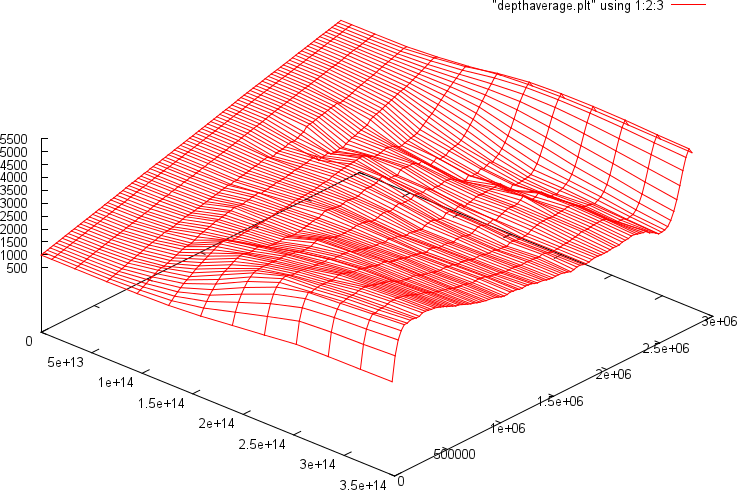
\includegraphics[width=0.6\textwidth]{depthaverage2}
  \caption{\it Example output for depth average statistics. On the left axis are 13 time steps, on the right is the depth (from the top at 0 to the bottom of the mantle on the far right), and the upwards pointing axis is the average temperature. This plot is created by calling \texttt{splot "depthaverage.plt" using 1:2:3 with lines} in gnuplot.}
  \label{fig:depthaverage}
\end{figure}

\end{itemize}



\subsection{Selecting between 2d and 3d runs}
\label{sec:2d-vs-3d}

\aspect{} can solve both two- and three-dimensional problems. You
select which one you want by putting a line like the following into
\index[prmindex]{Dimension}
\index[prmindexfull]{Dimension}
the parameter file (see Section~\ref{sec:parameters}):
\begin{lstlisting}[frame=single,language=prmfile]
set Dimension                     = 2
\end{lstlisting}

Internally, dealing with the dimension builds on a feature in
\dealii{}, upon which \aspect{} is based, that is called
\textit{dimension-independent programming}. In essence, what this does is that
you write your code only once in a way so that the space dimension is a
variable (or, in fact, a template parameter) and you can compile the code for
either 2d or 3d. The advantage is that codes can be tested and debugged in 2d
where simulations are relatively cheap, and the same code can then be
re-compiled and executed in 3d where simulations would otherwise be
prohibitively expensive for finding bugs; it is also a useful feature when
scoping out whether certain parameter settings will have the desired effect by
testing them in 2d first, before running them in 3d. This feature is discussed
in detail in the
\href{http://www.dealii.org/developer/doxygen/deal.II/step_4.html}{\dealii{}
  tutorial program step-4}.
Like there, all the functions and classes in
\aspect{} are compiled for both 2d and 3d. Which dimension is actually
called internally depends on what you have set in the input file, but
in either case, the machine code generated for 2d and 3d results from
the same source code and should, thus, contain the same set of
features and bugs. Running in 2d and 3d should therefore yield
comparable results. Be prepared to wait much longer for
computations to finish in the latter case, however.


\subsection{Debug or optimized mode}
\label{sec:debug-mode}

\aspect{} utilizes a \dealii{} feature called \textit{debug
  mode}. By default, \aspect{} uses debug mode, i.e., it calls a version of
the \dealii{} library that contain lots of checks for the correctness of
function arguments, the consistency of the internal state of data structure,
etc. If you program with \dealii{}, for example to extend \aspect{}, it has
been our experience over the years that, by number, most programming errors are of the
kind where one forgets to initialize a vector, one accesses data that has not
been updated, one tries to write into a vector that has ghost elements,
etc. If not caught, the result of these bugs is that parts of the program use
invalid data (data written into ghost elements is not communicated to other
processors), that operations simply make no sense (adding vectors of different
length), that memory is corrupted (writing past the end of an array) or, in
rare and fortunate cases, that the program simply crashes.

Debug mode is designed to catch most of these errors: It enables some 7,300
assertions (as of late 2011) in \dealii{} where we check for errors like the
above and, if the condition is violated, abort the program with a detailed
message that shows the failed check, the location in the source code, and a
stacktrace how the program got there. The downside of debug mode is, of
course, that it makes the program much slower -- depending on application by a
factor of 4--10. An example of the speedup one can get is shown in
Section~\ref{sec:cookbooks-simple-box}.

\aspect{} by default uses debug mode because most users will want to play with
the source code, and because it is also a way to verify that the compilation
process worked correctly. If you have verified that the program runs correctly
with your input parameters, for example by letting it run for the first 10
time steps, then you can switch to optimized mode by editing the top of the
\url{Makefile} and following the steps to build and run in
Section~\ref{sec:compiling}; alternatively, you can just build the entire
application using the command {\tt{make debug-mode=off}}.

\note{It goes without saying that if you make significant modifications to the
  program, you should do the first runs in debug mode to verify that your
  program still works as expected.}


\subsection{Visualizing results}
\label{sec:viz}

Among the postprocessors that can be selected in the input parameter file (see
Sections~\ref{sec:running-overview} and
\ref{parameters:Postprocess/Visualization}) are some that can produce files in
a format that can later be used to generate a graphical visualization of the
solution variables $\mathbf u, p$ and $T$ at select time steps, or of
quantities derived from these variables (for the latter, see
Section~\ref{sec:viz-postpostprocessors}).

By default, the files that are generated are in VTU format, i.e., the
XML-based, compressed format defined by the VTK library, see
\url{http://public.kitware.com/VTK/}. This file format has become a broadly
accepted pseudo-standard that many visualization program support, including
two of the visualization programs used most widely in computational science:
Visit (see \url{http://www.llnl.gov/visit/}) and ParaView (see
\url{http://www.paraview.org/HTML/Index.html}). The VTU format has a number of
advantages beyond being widely distributed:
\begin{itemize}
\item It allows for compression, keeping files relatively small even for
  sizeable computations.
\item It is a structured XML format, allowing other programs to read it
  without too much trouble.
\item It has a degree of support for parallel computations where every
  processor would only write that part of the data to a file that this
  processor in fact owns, avoiding the need to communicate all data to a
  single processor that then generates a single file. This requires a master
  file for each time step that then contains a reference to the individual
  files that together make up the output of a single time step. Unfortunately,
  there doesn't appear to be a standard for these master records; however,
  both ParaView and Visit have defined a format that each of these programs
  understand and that requires placing a file with ending \texttt{.pvtu} or
  \texttt{.visit} into the same directory as the output files from each
  processor. Section~\ref{sec:running-overview} gives an example of what can
  be found in the output directory.
\end{itemize}

\note{You can select other formats for output than VTU, see the run-time
  parameters in Section~\ref{parameters:Postprocess/Visualization}. However,
  none of the numerous formats currently implemented in \dealii{} other than
  the VTK/VTU formats allows for splitting up data over multiple files in case
  of parallel computations, thus making subsequent visualization of the entire
  volume impossible. Furthermore, given the amount of data \aspect{} can
  produce, the compression that is part of the VTU format is an important part
  of keeping data manageable.
\index[prmindex]{Output format}
\index[prmindexfull]{Postprocess!Visualization!Output format}
}

\subsubsection{Visualization the graphical output using \textit{Visit}}
In the following, let us discuss the process of visualizing a 2d computation
using Visit. The steps necessary for other visualization programs will
obviously differ but are, in principle, similar.

To this end, let us consider a simulation of convection in a box-shaped, 2d
region (see the ``cookbooks'' section, Section~\ref{sec:cookbooks}, and in
particular Section~\ref{sec:cookbooks-simple-box} for
the input file for this particular model). We can run the program with 4 processors using
\begin{verbatim}
  mpirun -np 4 ./lib/aspect-2d box.prm
\end{verbatim}
Letting the program run for a while will result in several output files as
discussed in Section~\ref{sec:running-overview} above.

In order to visualize one time step, follow these steps:%
\footnote{The instructions and screenshots were generated with Visit
  2.1. Later versions of Visit differ slightly in the arrangement of
  components of the graphical user interface, but the workflow and general
  idea remains unchanged.}

\begin{figure}[tbp]
  \phantom{.}
  \hfill
  \subfigure[]{
    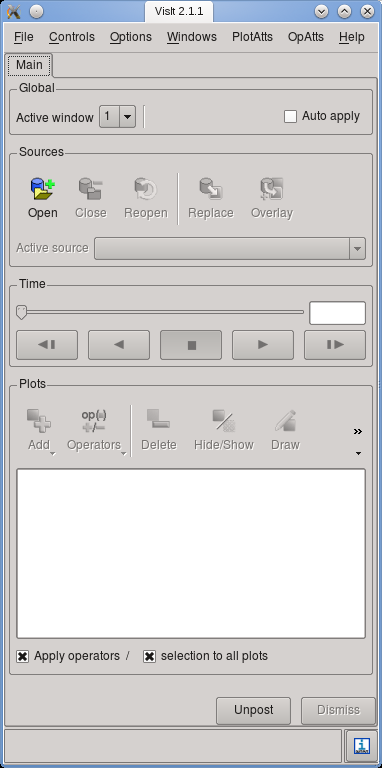
\includegraphics[width=0.24\textwidth]{viz/visit/visit-1}
    \label{fig:visit-1:a}
  }
  \hfill
  \subfigure[]{
    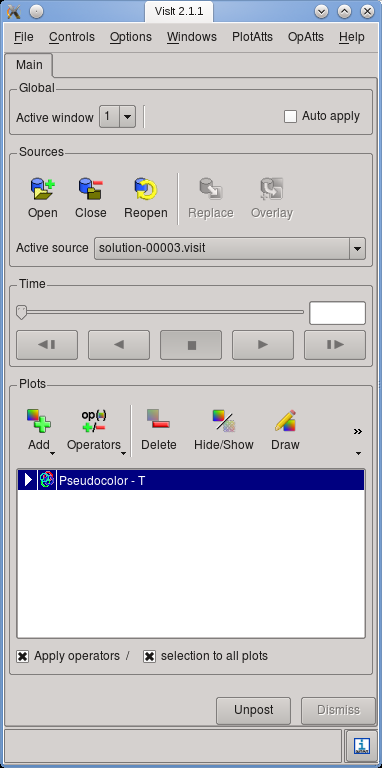
\includegraphics[width=0.24\textwidth]{viz/visit/visit-2}
    \label{fig:visit-1:b}
  }
  \hfill
  \subfigure[]{
    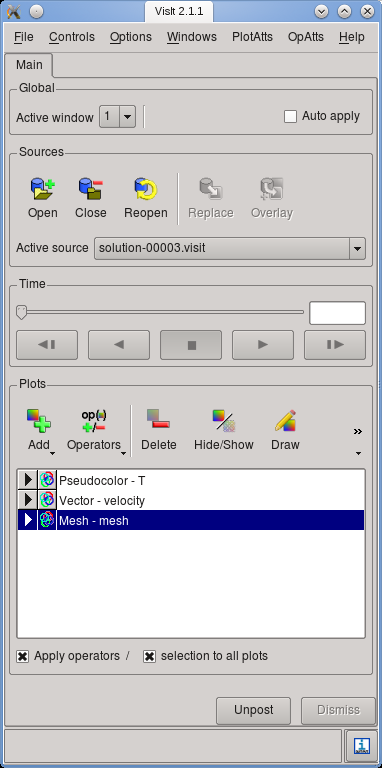
\includegraphics[width=0.24\textwidth]{viz/visit/visit-3}
    \label{fig:visit-1:c}
  }
  \hfill
  \phantom{.}
  \caption{\it Main window of Visit, illustrating the different steps of
    adding content to a visualization.}
  \label{fig:visit-1}
\end{figure}

\begin{figure}[tbp]
  \phantom{.}
  \hfill
  \subfigure[]{
    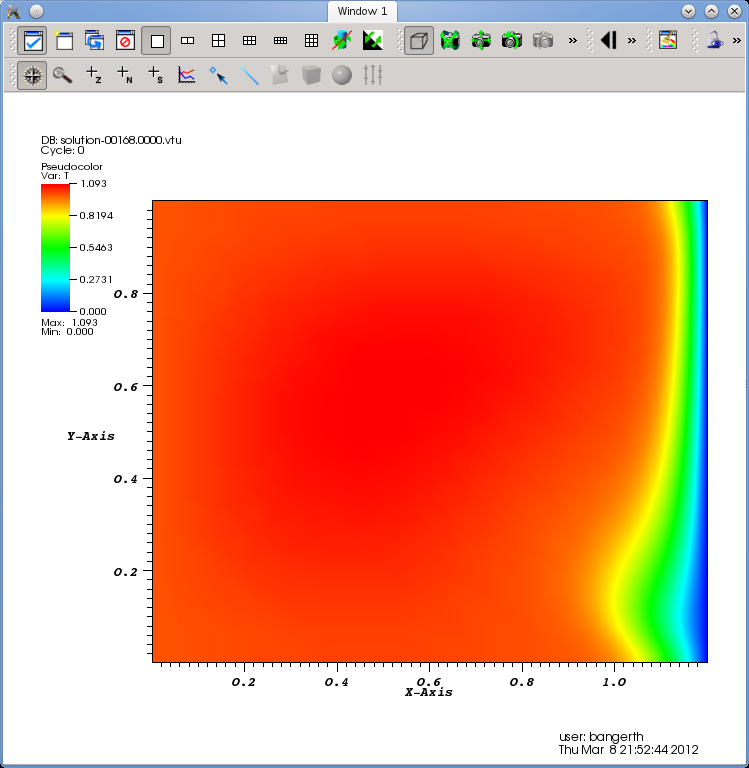
\includegraphics[width=0.48\textwidth]{viz/visit/visit-4}
    \label{fig:visit-2:a}
  }
  \hfill
  \subfigure[]{
    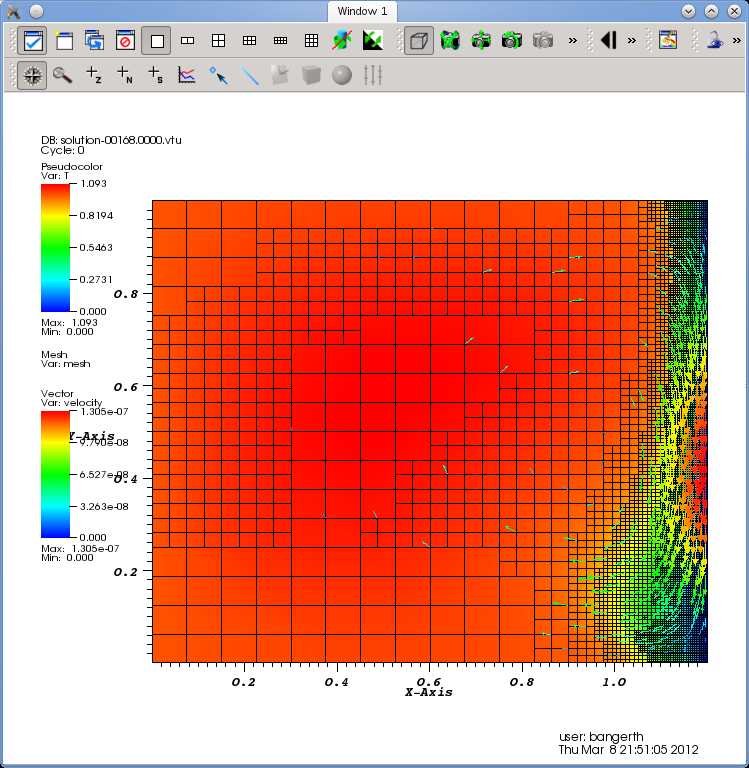
\includegraphics[width=0.48\textwidth]{viz/visit/visit-5}
    \label{fig:visit-2:b}
  }
  \hfill
  \phantom{.}
  \caption{\it Display window of Visit, showing a single plot and one where
    different data is overlaid.}
  \label{fig:visit-2}
\end{figure}

\begin{itemize}
\item \textit{Selecting input files:} As mentioned above, in parallel
  computations we usually generate one output file per processor in each time
  step for which visualization data is produced (see, however,
  Section~\ref{sec:viz-data}). To tell Visit which files together make up one
  time step, \aspect{} creates a \texttt{solution-NNNNN.visit} file in the
  output directory. To open it, start Visit, click on the ``Open'' button in
  the ``Sources'' area of
  its main window (see Fig.~\ref{fig:visit-1:a}) and select the file you
  want. Alternatively, you can also select files using the ``File $>$ Open''
  menu item, or hit the corresponding keyboard short-cut. After adding an
  input source, the ``Sources'' area of the main window should list the
  selected file name.

\item \textit{Selecting what to plot:} \aspect{} outputs all sorts of
  quantities that characterize the solution, such as temperature, pressure,
  velocity, and many others on demand (see
  Section~\ref{parameters:Postprocess/Visualization}). Once an input file has
  been opened, you will want to add graphical representations of some of this
  data to the still empty canvas. To this end, click on the ``Add'' button of
  the ``Plots'' area. The resulting menu provides a number of different kinds
  of plots. The most important for our purpose are: (i) ``Pseudocolor'' allows
  the visualization of a scalar field (e.g., temperature, pressure, density)
  by using a color field. (ii) ``Vector'' displays a vector-valued field
  (e.g., velocity) using arrows. (iii) ``Mesh'' displays the mesh. The
  ``Contour'', ``Streamline'' and ``Volume'' options are also frequently
  useful, in particular in 3d.

  Let us choose the ``Pseudocolor'' item and select the temperature field as
  the quantity to plot. Your main window should now look as shown in
  Fig.~\ref{fig:visit-1:b}. Then hit the ``Draw'' button to make Visit generate
  data for the selected plots. This will yield a picture such as shown in
  Fig.~\ref{fig:visit-2:a} in the display window of Visit.

\item \textit{Overlaying data:} Visit can overlay multiple plots in the same
  view. To this end, add another plot to the view using again the ``Add''
  button to obtain the menu of possible plots, then the ``Draw'' button to
  actually draw things. For example, if we add velocity vectors and the mesh,
  the main window looks as in Fig.~\ref{fig:visit-1:c} and the main view as in
  Fig.~\ref{fig:visit-2:b}.

\item \textit{Adjusting how data is displayed:} Without going into too much
  detail, if you double click onto the name of a plot in the ``Plots'' window,
  you get a dialog in which many of the properties of this plot can be
  adjusted. Further details can be changed by using ``Operators'' on a plot.

\item \textit{Making the output prettier:} As can be seen in
  Fig.~\ref{fig:visit-2}, Visit by default puts a lot of clutter around the
  figure -- the name of the user, the name of the input file, color bars, axes
  labels and ticks, etc. This may be useful to explore data in the beginning
  but does not yield good pictures for presentations or publications. To
  reduce the amount of information displayed, go to the ``Controls $>$
  Annotations'' menu item to get a dialog in which all of these displays can
  be selectively switched on and off.

\item \textit{Saving figures:} To save a visualization into a file that can
  then be included into presentations and publications, go to the menu item
  ``File $>$ Save window''. This will create successively numbered files in
  the directory from which Visit was started each time a view is saved. Things
  like the format used for these files can be chosen using the ``File $>$ Set
  save options'' menu item. We have found that one can often get better
  looking pictures by selecting the ``Screenshot'' method in this dialog.
\end{itemize}

More information on all of these topis can be found in the Visit
documentation, see \url{http://www.llnl.gov/visit/}. We have also recorded
video lectures demonstrating this process interactively at
\url{http://www.youtube.com/watch?v=3ChnUxqtt08} for Visit, and at
\url{http://www.youtube.com/watch?v=w-65jufR-bc} for Paraview.


\subsubsection{Visualizing statistical data}
\label{sec:viz-stat}

In addition to the graphical outputdiscussed above, \aspect{} produces a
statistics file that collects information produced during each time step.
For the remainder of this section, let us assume that we have run \aspect{}
with the input file discussed in Section~\ref{sec:cookbooks-simple-box},
simulating convection in a box. After running \aspect{}, you will find
a file called \texttt{statistics} in the output directory that, at the time
of writing this, looked like this:
This file has a structure that looks like this:
  \begin{lstlisting}[frame=single,language=ksh]
# 1: Time step number
# 2: Time (seconds)
# 3: Number of mesh cells
# 4: Number of Stokes degrees of freedom
# 5: Number of temperature degrees of freedom
# 6: Iterations for temperature solver
# 7: Iterations for Stokes solver
# 8: Time step size (seconds)
# 9: RMS velocity (m/s)
# 10: Max. velocity (m/s)
# 11: Minimal temperature (K)
# 12: Average temperature (K)
# 13: Maximal temperature (K)
# 14: Average nondimensional temperature (K)
# 15: Outward heat flux through boundary with indicator 0 (W)
# 16: Outward heat flux through boundary with indicator 1 (W)
# 17: Outward heat flux through boundary with indicator 2 (W)
# 18: Outward heat flux through boundary with indicator 3 (W)
# 19: Visualization file name
   0 0.0000e+00 256 2467 1089  1 22 1.2225e-02 1.79038621e+00 2.54812273e+00 ...
   1 1.2225e-02 256 2467 1089 40 16 3.7409e-03 5.88727814e+00 8.34299267e+00 ...
   2 1.5966e-02 256 2467 1089 25 15 2.0249e-03 1.08925316e+01 1.54185045e+01 ...
   3 1.7991e-02 256 2467 1089 19 15 1.3658e-03 1.61586242e+01 2.28690070e+01 ...
   4 1.9357e-02 256 2467 1089 16 14 1.0291e-03 2.14311381e+01 3.03519178e+01 ...
   5 2.0386e-02 256 2467 1089 14 14 8.2853e-04 2.65966688e+01 3.76989179e+01 ...
  \end{lstlisting}

In other words, it first lists what the individual columns mean with a hash
mark at the beginning of the line and then has one line for each time step
in which the individual columns list what has been explained above. In the
example shown here, the first time step appears twice because we use a mesh
that starts out globally refined and we then start the entire computation
over again on a once adaptively refined mesh (see the parameters in
Section~\ref{parameters:Mesh_20refinement} for how to do that).

This file is easy to visualize. For example, one can import it as a whitespace
separated file into a spreadsheet such as Microsoft Excel or OpenOffice/LibreOffice
Calc and then generate graphs of one column against another. Or, maybe simpler,
there is a multitude of simple graphing programs that do not need the overhead
of a full fledged spreadsheet engine and simply plot graphs. One that is
particularly simple to use and available on every major platform is \texttt{Gnuplot}.
It is extensively documented at \url{http://www.gnuplot.info/}.

\texttt{Gnuplot} is a command line program in which you enter commands that
plot data or modify the way data is plotted. When you call it, you will first
get a screen that looks like this:
\begin{lstlisting}[frame=single]
/home/user/aspect/output$ gnuplot

        G N U P L O T
        Version 4.6 patchlevel 0    last modified 2012-03-04
        Build System: Linux x86_64

        Copyright (C) 1986-1993, 1998, 2004, 2007-2012
        Thomas Williams, Colin Kelley and many others

        gnuplot home:     http://www.gnuplot.info
        faq, bugs, etc:   type "help FAQ"
        immediate help:   type "help"  (plot window: hit 'h')

Terminal type set to 'qt'
gnuplot>
\end{lstlisting}
At the prompt on the last line, you can then enter commands. Given the
description of the individual columns given above, let us first try to
plot the heat flux through boundary 2 (which in this case is the bottom
boundary of the box), i.e., column 17, as a function of time (column 2).
This can be achieved using the following command:
\begin{lstlisting}[frame=single,language=gnuplot]
  plot "statistics" using 2:17
\end{lstlisting}
The left panel of Fig.~\ref{fig:viz-gnuplot-1} shows what \texttt{Gnuplot}
will display in its output window. There are many things one can
configure in these plots (see the \texttt{Gnuplot} manual referenced above).
For example, let us assume that we want to add labels to the $x$- and $y$-axes,
use not just points but lines and points for the curves,
restrict the time axis to the range $[0,0.2]$ and the heat flux axis to
$[-10:10]$,
plot not only the flux through the bottom but also through the top boundary
(column 18) and finally add a key to the figure, then the following
commands achieve this:
\begin{lstlisting}[frame=single,language=gnuplot]
  set xlabel "Time"
  set ylabel "Heat flux"
  set style data linespoints
  plot [0:0.2][-10:10] "statistics" using 2:17 title "Bottom boundary", \
                       "statistics" using 2:18 title "Top boundary"
\end{lstlisting}
If a line gets too long, you can continue it by ending it in a backslash as
above. This is rarely used on the command line but useful when writing the
commands above into a script file, see below. We have done it here to get
the entire command into the width of the page.

\begin{figure}
  \centering
  \phantom.
  \hfill
  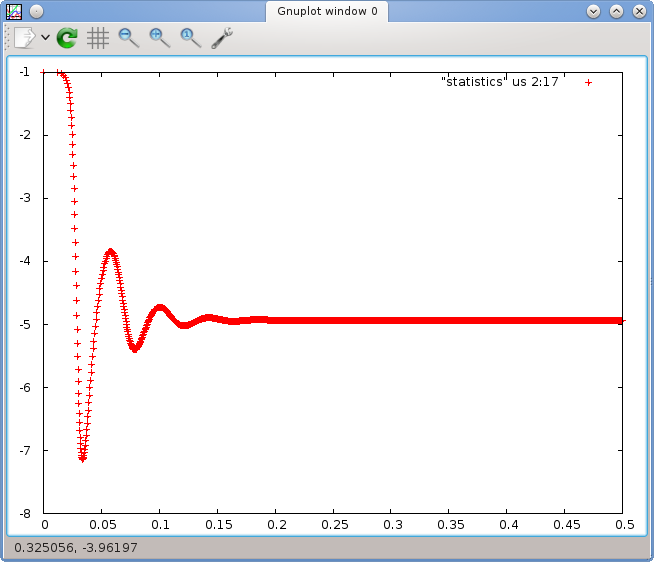
\includegraphics[width=0.4\textwidth]{viz/statistics/1}
  \hfill
  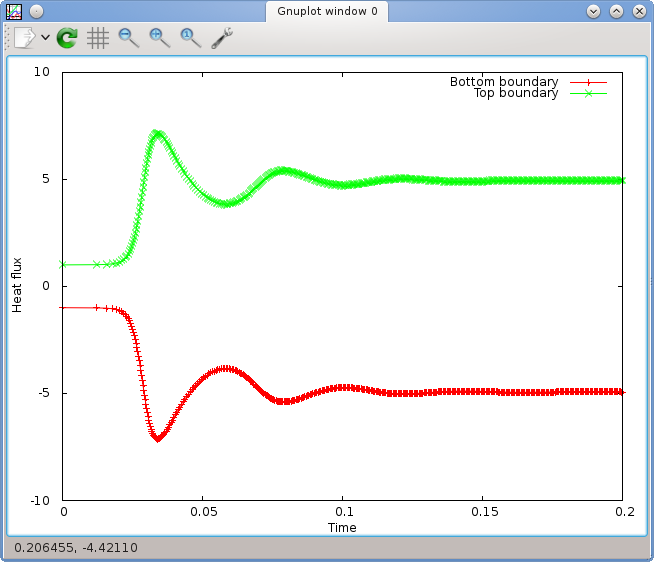
\includegraphics[width=0.4\textwidth]{viz/statistics/2}
  \hfill
  \phantom.
  \caption{\it Visualizing the statistics file obtained from the example in
    Section~\ref{sec:cookbooks-simple-box} using \texttt{Gnuplot}: Output
    using simple commands.}
  \label{fig:viz-gnuplot-1}
\end{figure}

For those who are lazy, \texttt{Gnuplot} allows to abbreviate things in many
different ways. For example, one can abbreviate most commands. Furthermore,
one does not need to repeat the name of an input file if it is the same
as the previous one in a plot command. Thus, instead of the commands above,
the following abbreviated form would have achieved the same effect:
\begin{lstlisting}[frame=single,language=gnuplot]
  se xl "Time"
  se yl "Heat flux"
  se sty da lp
  pl [:0.2][-10:10] "statistics" us 2:17 t "Bottom boundary", "" us 2:18 t "Top boundary"
\end{lstlisting}
This is of course unreadable at first but becomes useful once you become
more familiar with the command offered by this program.

Once you have gotten the commands that create the plot you want right, you probably
want to save it into a file. \texttt{Gnuplot} can write output in many
different formats. For inclusion in publications, either \texttt{eps} or
\texttt{png} are the most common. In the latter case, the commands to
achieve this are
\begin{lstlisting}[frame=single,language=gnuplot]
  set terminal png
  set output "heatflux.png"
  replot
\end{lstlisting}
The last command will simply generate the same plot again but this time
into the given file. The result is a graphics file similar to the one
shown in Fig.~\ref{fig:convection-box-stats} on page \pageref{fig:convection-box-stats}.

\note{After setting output to a file, \textit{all} following plot commands will
	want to write to this file. Thus, if you want to create more plots after
	the one just created, you need to reset output back to the screen. On linux,
	this is done using the command \texttt{set terminal X11}. You can then
	continue experimenting with plots and when you have the next plot ready,
	switch back to output to a file.}

What makes \texttt{Gnuplot} so useful is that it doesn't just allow entering
all these commands at the prompt. Rather, one can write them all into a file,
say \texttt{plot-heatflux.gnuplot}, and then, on the command line, call
\begin{lstlisting}[frame=single,language=ksh]
  gnuplot plot-heatflux.gnuplot
\end{lstlisting}
to generate the \texttt{heatflux.png} file. This comes in handy if one wants
to create the same plot for multiple simulations while playing with parameters
of the physical setup. It is also a very useful tool if one wants to generate
the same kind of plot again later with a different data set, for example when
a reviewer requested additional computations to be made for a paper or if one
realizes that one has forgotten or misspelled an axis label in a plot.%
\footnote{In my own work, I usually save the \aspect{} input file, the
  \texttt{statistics} output file and the \texttt{Gnuplot} script along with
  the actual figure I want to include in a paper. This way, it is easy to
  either re-run an entire simulation, or just tweak the graphic at a later
  time. Speaking from experience, you will not believe how often one wants
  to tweak a figure long after it was first created. In such situations it is
  outstandingly helpful if one still has both the actual data as well as the script
  that generated the graphic.}

\texttt{Gnuplot} has many many more features we have not even touched upon. For
example, it is equally happy to produce three-dimensional graphics, and it also
has statistics modules that can do things like curve fits, statistical regression,
and many more operations on the data you provide in the columns of an input file.
We will not try to cover them here but instead refer to the manual at
\url{http://www.gnuplot.info/}. You can also get a good amount of information
by typing \texttt{help} at the prompt, or a command like \texttt{help plot} to
get help on the \texttt{plot} command.


\subsubsection{Large data issues for parallel computations}
\label{sec:viz-data}

Among the challenges in visualizing the results of parallel computations is
dealing with the large amount of data. The first bottleneck this presents is
during run-time when \aspect{} wants to write the visualization data of a time
step to disk. Using the compressed VTU format, \aspect{} generates on the
order of 10 bytes of output for each degree of freedom in 2d and more in 3d;
thus, output of a single time step can run into the range of gigabytes that
somehow have to get from compute nodes to disk. This stresses both the cluster
interconnect as well as the data storage array.
\index[prmindex]{Number of grouped files}
\index[prmindexfull]{Postprocess!Visualization!Number of grouped files}


There are essentially two strategies supported by \aspect{} for this scenario:
\begin{itemize}
\item If your cluster has a fast interconnect, for example Infiniband, and if
  your cluster has a fast, distributed file system, then \aspect{} can produce
  output files that are already located in the correct output directory (see
  the options in Section~\ref{parameters:global}) on the global file
  system. \aspect{} uses MPI I/O calls to this end, ensuring that the local
  machines do not have to access these files using slow NFS-mounted global
  file systems.

\item If your cluster has a slow interconnect, e.g., if it is simply a
  collection of machines connected via ethernet, then writing data to a
  central file server may block the rest of the program for a while. On the
  other hand, if your machines have fast local storage for temporary file
  systems, then \aspect{} can write data first into such a file and then move
  it in the background to its final destination while already continuing
  computations. To select this mode, set the appropriate variables discussed
  in Section~\ref{parameters:Postprocess/Visualization}. Note, however, that
  this scheme only makes sense if every machine on which MPI processes run has
  fast local disk space for temporary storage.
\end{itemize}

\note{An alternative would be if every processor directly writes its own files
  into the global output directory (possibly in the background), without the
  intermediate step of the temporary file. In our experience, file servers are
  quickly overwhelmed when encountering a few hundred machines wanting to
  open, fill, flush and close their own file via NFS mounted file system
  calls, sometimes completely blocking the entire cluster environment for
  extended periods of time.}

\subsection{Checkpoint/restart support}

If you do long runs, especially when using parallel computations, there are a
number of reasons to periodically save the state of the program:
\begin{itemize}
\item If the program crashes for whatever reason, the entire computation may
  be lost. A typical reason is that a program has exceeded the requested
  wallclock time allocated by a batch scheduler on a cluster.
\item Most of the time, no realistic initial conditions for strongly
  convecting flow are available. Consequently, one typically starts with a
  somewhat artificial state and simply waits for a long while till the
  convective state enters the phase where it shows its long-term
  behavior. However, getting there may take a good amount of CPU time and it
  would be silly to always start from scratch for each different parameter
  setting. Rather, one would like to start such parameter studies with a saved
  state that has already passed this initial, unphysical, transient stage.
\end{itemize}

To this end, \aspect{} creates a set of files in the output directory
\index[prmindex]{Output directory}
\index[prmindexfull]{Output directory}
(selected in the parameter file) every 50 time steps in which the entire state
of the program is saved so that a simulation can later be continued at this
point. The previous checkpoint files will then be deleted. To resume
operations from the last saved state, you need to set the \texttt{Resume
  computation} flag in the input parameter file to \texttt{true}, see
\index[prmindex]{Resume computation}
\index[prmindexfull]{Resume computation}
Section~\ref{parameters:global}.

\note{It is not imperative that the parameters selected in the input file are
  exactly the same when resuming a program from a saved state than what they
  were at the time when this state was saved. For example, one may want to
  choose a different parametrization of the material law, or add or remove
  postprocessors that should be run at the end of each time step. Likewise,
  the end time, the times at which some additional mesh refinement steps
  should happen, etc., can be different.

  Yet, it is
  clear that some other things can't be changed: For example, the geometry
  model that was used to generate the coarse mesh and describe the boundary
  must be the same before and after resuming a computation. Likewise, you can
  not currently restart a computation with a different number of processors
  than initially used to checkpoint the simulation.
  Not all invalid
  combinations are easy to detect, and \aspect{} may not always realize
  immediate what is going on if you change a setting that can't be
  changed. However, you will almost invariably get non-sensical results after
  some time.}


\section{Run-time input parameters}
\label{sec:parameters}

\subsection{Overview}
\label{sec:parameters-overview}

What \aspect{} computes is driven by two things:
\begin{itemize}
\item The models implemented in \aspect{}. This includes the geometries, the
  material laws, or the initial conditions currently supported. Which of these
  models are currently implemented is discussed below;
  Section~\ref{sec:extending} discusses in great detail the process of
  implementing additional models.

\item Which of the implemented models is selected, and what their run-time
  parameters are. For example, you could select a model that prescribes
  constant coefficients throughout the domain from all the material models
  currently implemented; you could then select appropriate values for all of
  these constants. Both of these selections happen from a parameter file that
  is read at run time and whose name is specified on the command line. (See
  also Section~\ref{sec:running-overview}.)
\end{itemize}
In this section, let us give an overview of what can be selected in the
parameter file. Specific parameters, their default values, and allowed values
for these parameters are documented in the following subsections. An index
with page numbers for all run-time parameters can be found on
page~\pageref{sec:runtime-parameter-index}.

\subsubsection{The structure of parameter files}

Most of the run-time behavior of \aspect{} is driven by a parameter file that
looks in essence like this:
\begin{lstlisting}[frame=single,language=prmfile]
set Dimension                     = 2
set Resume computation            = false
set End time                      = 1e10
set CFL number                    = 1.0
set Output directory              = bin

subsection Mesh refinement
  set Initial adaptive refinement = 1
  set Initial global refinement   = 4
end

subsection Material model
  set Model name                  = simple

  subsection Simple model
    set Reference density         = 3300
    set Reference temperature     = 293
    set Viscosity                 = 5e24
  end
end

...
\end{lstlisting}

Some parameters live at the top level, but most parameters are grouped into
subsections. An input parameter file is therefore much like a file system: a
few files live in the root directory; others are in a nested hierarchy of
sub-directories. And just as with files, parameters have both a name (the
thing to the left of the equals sign) and a content (what's to the right).

All parameters you can list in this input file have been \textit{declared} in
\aspect. What this means is that you can't just list anything in the input
file with entries that are unknown simply being ignored. Rather, if your input
file contains a line setting a parameter that is unknown to something, you
will get an error message. Likewise, all declared parameters have a
description of possible values associated with them -- for example, some
parameters must be non-negative integers (the number of initial refinement
steps), can either be true or false (whether the computation should be resumed
from a saved state), or can only be a single element from a selection (the
name of the material model). If an entry in your input file doesn't satisfy
these constraints, it will be rejected at the time of reading the file (and
not when a part of the program actually accesses the value and the programmer
has taken the time to also implement some error checking at this location).
Finally, because parameters have been declared, you do not \textit{need} to
specify a parameter in the input file: if a parameter isn't listed, then the
program will simply use the default provided when declaring the parameter.

\subsubsection{Categories of parameters}

The parameters that can be provided in the input file can roughly be
categorized into the following groups:
\begin{itemize}
\item Global parameters (see Section~\ref{parameters:global}): These
  parameters determine the overall behavior of the program. Primarily they
  describe things like the output directory, the end time of the simulation,
  or whether the computation should be resumed from a previously saved state.

\item Parameters for certain aspects of the numerical algorithm: These
  describe, for example, the specifics of the spatial discretization. In
  particular, this is the case for parameters concerning
  the polynomial degree of the finite element approximation
  (Section~\ref{parameters:Discretization}), some details about the
  stabilization
  (Section~\ref{parameters:Discretization/Stabilization_20parameters}), and
  how adaptive mesh refinement is supposed to work
  (Section~\ref{parameters:Mesh_20refinement}).

\item Parameters that describe certain global aspects of the equations to be
  solved: This includes, for example, a description if certain terms in the
  model should be omitted or not. See
  Section~\ref{parameters:Model_20settings} for the list of parameters in this
  category.

\item Parameters that characterize plugins: Certain behaviors of
  \aspect{} are described by what we call \textit{plugins} -- self-contained
  parts of the code that describe one particular aspect of the simulation. An
  example would be which of the implemented material models to use, and the
  specifics of this material model. The sample parameter file above gives an
  indication of how this works: within a subsection of the file that pertains
  to the material models, one can select one out of several plugins (or, in
  the case of the postprocessors, any number, including none, of the available
  plugins), and one can then specify the specifics of this model in a
  sub-subsection dedicated to this particular model.

  A number of components of \aspect{} are implemented via plugins. These are,
  together with the sections in which their parameters are declared:
  \begin{itemize}
  \item The material model:
    Sections~\ref{parameters:Material_20model} and following.
  \item The geometry:
    Sections~\ref{parameters:Geometry_20model} and following.
  \item The gravity description:
    Sections~\ref{parameters:Gravity_20model} and following.
  \item Initial conditions for the temperature:
    Sections~\ref{parameters:Initial_20conditions} and following.
  \item Temperature boundary conditions:
    Sections~\ref{parameters:Boundary_20temperature_20model} and following.
  \item Postprocessors:
    Sections~\ref{parameters:Postprocess} and following for most postprocessors,
    section \ref{parameters:Postprocess/Visualization} and following for
    postprocessors related to visualization.
  \end{itemize}
\end{itemize}

The details of parameters in each of these categories can be found in the
sections linked to above. Some of them will also be used in the cookbooks in
Section~\ref{sec:cookbooks}.


% now include a file that describes all currently available run-time parameters
\subsection{Global parameters}
\label{parameters:global}


\begin{itemize}
\item {\it Parameter name:} {\tt CFL number}


{\it Value:} 1.0


{\it Default:} 1.0


{\it Description:} In computations, the time step $k$ is chosen according to $k = c \min_K \frac{h_K}{\|u\|_{\infty,K} p_T}$ where $h_K$ is the diameter of cell $K$, and the denominator is the maximal magnitude of the velocity on cell $K$ times the polynomial degree $p_T$ of the temperature discretization. The dimensionless constant $c$ is called the CFL number in this program. For time discretizations that have explicit components, $c$ must be less than a constant that depends on the details of the time discretization and that is no larger than one. On the other hand, for implicit discretizations such as the one chosen here, one can choose the time step as large as one wants (in particular, one can choose $c>1$) though a CFL number significantly larger than one will yield rather diffusive solutions. Units: None.


{\it Possible values:} [Double 0...1.79769e+308 (inclusive)]
\item {\it Parameter name:} {\tt End time}


{\it Value:} 2e8


{\it Default:} 1e8


{\it Description:} The end time of the simulation. Units: years.


{\it Possible values:} [Double 0...1.79769e+308 (inclusive)]
\item {\it Parameter name:} {\tt Output directory}


{\it Value:} output


{\it Default:} output


{\it Description:} The name of the directory into which all output files should be placed. This may be an absolute or a relative path.


{\it Possible values:} [DirectoryName]
\item {\it Parameter name:} {\tt Resume computation}


{\it Value:} false


{\it Default:} false


{\it Description:} A flag indicating whether the computation should be resumed from a previously saved state (if true) or start from scratch (if false).


{\it Possible values:} [Bool]
\end{itemize}



\subsection{Parameters in section \tt Boundary temperature model}
\label{parameters:Boundary_20temperature_20model}

\begin{itemize}
\item {\it Parameter name:} {\tt Model name}


{\it Value:} box


{\it Default:}


{\it Description:} Select one of the following models:

`spherical constant': A model in which the temperature is chosen constant on the
inner and outer boundaries of a spherical shell. Parameters are read from
subsection 'Spherical constant'.

`box': A model in which the temperature is chosen constant on the left and right sides of a box.


{\it Possible values:} [Selection spherical constant|box ]
\end{itemize}



\subsection{Parameters in section \tt Boundary temperature model/Spherical constant}
\label{parameters:Boundary_20temperature_20model/Spherical_20constant}

\begin{itemize}
\item {\it Parameter name:} {\tt Inner temperature}


{\it Value:} 6300


{\it Default:} 6000


{\it Description:} Temperature at the inner boundary (core mantle boundary). Units: K.


{\it Possible values:} [Double -1.79769e+308...1.79769e+308 (inclusive)]
\item {\it Parameter name:} {\tt Outer temperature}


{\it Value:} 300


{\it Default:} 0


{\it Description:} Temperature at the outer boundary (lithosphere water/air). Units: K.


{\it Possible values:} [Double -1.79769e+308...1.79769e+308 (inclusive)]
\end{itemize}

\subsection{Parameters in section \tt Discretization}
\label{parameters:Discretization}

\begin{itemize}
\item {\it Parameter name:} {\tt Stokes velocity polynomial degree}


{\it Value:} 2


{\it Default:} 2


{\it Description:} The polynomial degree to use for the velocity variables in the Stokes system. Units: None.


{\it Possible values:} [Integer range 1...2147483647 (inclusive)]
\item {\it Parameter name:} {\tt Temperature polynomial degree}


{\it Value:} 2


{\it Default:} 2


{\it Description:} The polynomial degree to use for the temperature variable. Units: None.


{\it Possible values:} [Integer range 1...2147483647 (inclusive)]
\item {\it Parameter name:} {\tt Use locally conservative discretization}


{\it Value:} false


{\it Default:} true


{\it Description:} Whether to use a Stokes discretization that is locally conservative at the expense of a larger number of degrees of freedom (true), or to go with a cheaper discretization that does not locally conserve mass, although it is globally conservative (false).


{\it Possible values:} [Bool]
\end{itemize}



\subsection{Parameters in section \tt Discretization/Stabilization parameters}
\label{parameters:Discretization/Stabilization_20parameters}

\begin{itemize}
\item {\it Parameter name:} {\tt alpha}


{\it Value:} 2


{\it Default:} 2


{\it Description:} The exponent $\alpha$ in the entropy viscosity stabilization. Units: None.


{\it Possible values:} [Double 1...2 (inclusive)]
\item {\it Parameter name:} {\tt beta}


{\it Value:} 0.078


{\it Default:} 0.078


{\it Description:} The $\beta$ factor in the artificial viscosity stabilization. An appropriate value for 2d is 0.052 and 0.078 for 3d. Units: None.


{\it Possible values:} [Double 0...1.79769e+308 (inclusive)]
\item {\it Parameter name:} {\tt cR}


{\it Value:} 0.5


{\it Default:} 0.11


{\it Description:} The $c_R$ factor in the entropy viscosity stabilization. Units: None.


{\it Possible values:} [Double 0...1.79769e+308 (inclusive)]
\end{itemize}

\subsection{Parameters in section \tt Geometry model}
\label{parameters:Geometry_20model}

\begin{itemize}
\item {\it Parameter name:} {\tt Model name}


{\it Value:} box


{\it Default:}


{\it Description:} Select one of the following models:

`spherical shell': A geometry representing a spherical shell or a piece of it.
Inner and outer radii are read from the parameter file in subsection 'Spherical
shell'.

`box': A box geometry with fixed length 1 in each coordinate direction.


{\it Possible values:} [Selection spherical shell|box ]
\end{itemize}



\subsection{Parameters in section \tt Geometry model/Spherical shell}
\label{parameters:Geometry_20model/Spherical_20shell}

\begin{itemize}
\item {\it Parameter name:} {\tt Inner radius}


{\it Value:} 5698e3


{\it Default:} 3481000


{\it Description:} Inner radius of the spherical shell. Units: m.


{\it Possible values:} [Double 0...1.79769e+308 (inclusive)]
\item {\it Parameter name:} {\tt Opening angle}


{\it Value:} 180


{\it Default:} 360


{\it Description:} Opening angle in degrees of the section of the shell that we want to build. Units: degrees.


{\it Possible values:} [Double 0...360 (inclusive)]
\item {\it Parameter name:} {\tt Outer radius}


{\it Value:} 10415e3


{\it Default:} 6336000


{\it Description:} Outer radius of the spherical shell. Units: m.


{\it Possible values:} [Double 0...1.79769e+308 (inclusive)]
\end{itemize}

\subsection{Parameters in section \tt Gravity model}
\label{parameters:Gravity_20model}

\begin{itemize}
\item {\it Parameter name:} {\tt Model name}


{\it Value:} vertical


{\it Default:}


{\it Description:} Select one of the following models:

`vertical': A gravity model in which the gravity direction is vertically downward and at constant magnitude.

`radial constant': A gravity model in which the gravity direction is radially inward and at constant magnitude. The magnitude is read from the parameter file in subsection 'Radial constant'.

`radial earth-like': A gravity model in which the gravity direction is radially inward and with a magnitude that matches that of the earth at the core-mantle boundary as well as at the surface and in between is physically correct under the assumption of a constant density.


{\it Possible values:} [Selection vertical|radial constant|radial earth-like ]
\end{itemize}



\subsection{Parameters in section \tt Gravity model/Radial constant}
\label{parameters:Gravity_20model/Radial_20constant}

\begin{itemize}
\item {\it Parameter name:} {\tt Magnitude}


{\it Value:} 30


{\it Default:} 30


{\it Description:} Magnitude of the gravity vector in $m/s^2$. The direction is always radially outward from the center of the earth.


{\it Possible values:} [Double 0...1.79769e+308 (inclusive)]
\end{itemize}

\subsection{Parameters in section \tt Initial conditions}
\label{parameters:Initial_20conditions}

\begin{itemize}
\item {\it Parameter name:} {\tt Model name}


{\it Value:} perturbed box


{\it Default:}


{\it Description:} Select one of the following models:

`spherical hexagonal perturbation': An initial temperature field in which the temperature is perturbed following a six-fold pattern in angular direction from an otherwise spherically symmetric state.

`spherical gaussian perturbation': An initial temperature field in which the temperature is perturbed by a single Gaussian added to an otherwise spherically symmetric state. Additional parameters are read from the parameter file in subsection 'Spherical gaussian perturbation'.

`perturbed box': An initial temperature field in which the temperature is perturbed slightly from an otherwise constant value equal to one. The perturbation is chosen in such a way that the initial temperature is constant to one along the entire boundary.


{\it Possible values:} [Selection spherical hexagonal perturbation|spherical gaussian perturbation|perturbed box ]
\end{itemize}



\subsection{Parameters in section \tt Initial conditions/Spherical gaussian perturbation}
\label{parameters:Initial_20conditions/Spherical_20gaussian_20perturbation}

\begin{itemize}
\item {\it Parameter name:} {\tt Amplitude}


{\it Value:} 0.01


{\it Default:} 0.01


{\it Description:} The amplitude of the perturbation.


{\it Possible values:} [Double 0...1.79769e+308 (inclusive)]
\item {\it Parameter name:} {\tt Angle}


{\it Value:} 4.71238898038468985769


{\it Default:} 0e0


{\it Description:} The angle where the center of the perturbation is placed.


{\it Possible values:} [Double 0...1.79769e+308 (inclusive)]
\item {\it Parameter name:} {\tt Non-dimensional depth}


{\it Value:} 0.7


{\it Default:} 0.7


{\it Description:} The non-dimensional radial distance where the center of the perturbation is placed.


{\it Possible values:} [Double 0...1.79769e+308 (inclusive)]
\item {\it Parameter name:} {\tt Sigma}


{\it Value:} 0.2


{\it Default:} 0.2


{\it Description:} The standard deviation of the Gaussian perturbation.


{\it Possible values:} [Double 0...1.79769e+308 (inclusive)]
\item {\it Parameter name:} {\tt Sign}


{\it Value:} 1


{\it Default:} 1


{\it Description:} The sign of the perturbation.


{\it Possible values:} [Double -1.79769e+308...1.79769e+308 (inclusive)]
\end{itemize}

\subsection{Parameters in section \tt Material model}
\label{parameters:Material_20model}

\begin{itemize}
\item {\it Parameter name:} {\tt Model name}


{\it Value:} simple


{\it Default:}


{\it Description:} Select one of the following models:

`table': A material model that reads tables of pressure and temperature dependent material coefficients from files.

`simple': A simple material model that has constant values for all coefficients but the density. This model uses the formulation that assumes an incompressible medium despite the fact that the density follows the law $\rho(T)=\rho_0(1-\beta(T-T_{\text{ref}})$. The value for the components of this formula and additional parameters are read from the parameter file in subsection 'Simple model'.


{\it Possible values:} [Selection table|simple ]
\end{itemize}



\subsection{Parameters in section \tt Material model/Simple model}
\label{parameters:Material_20model/Simple_20model}

\begin{itemize}
\item {\it Parameter name:} {\tt Reference density}


{\it Value:} 1


{\it Default:} 3300


{\it Description:} Reference density $\rho_0$. Units: $kg/m^3$.


{\it Possible values:} [Double 0...1.79769e+308 (inclusive)]
\item {\it Parameter name:} {\tt Reference temperature}


{\it Value:} 1


{\it Default:} 293


{\it Description:} The reference temperature $T_0$. Units: $K$.


{\it Possible values:} [Double 0...1.79769e+308 (inclusive)]
\item {\it Parameter name:} {\tt Thermal conductivity}


{\it Value:} 4.7


{\it Default:} 4.7


{\it Description:} The value of the thermal conductivity $k$. Units: $W/m/K$.


{\it Possible values:} [Double 0...1.79769e+308 (inclusive)]
\item {\it Parameter name:} {\tt Thermal expansion coefficient}


{\it Value:} 2e-5


{\it Default:} 2e-5


{\it Description:} The value of the thermal expansion coefficient $\beta$. Units: $1/K$.


{\it Possible values:} [Double 0...1.79769e+308 (inclusive)]
\item {\it Parameter name:} {\tt Viscosity}


{\it Value:} 1


{\it Default:} 5e24


{\it Description:} The value of the constant viscosity. Units: $kg/m/s$.


{\it Possible values:} [Double 0...1.79769e+308 (inclusive)]
\end{itemize}

\subsection{Parameters in section \tt Mesh refinement}
\label{parameters:Mesh_20refinement}

\begin{itemize}
\item {\it Parameter name:} {\tt Additional refinement times}


{\it Value:}


{\it Default:}


{\it Description:} A list of times so that if the end time of a time step is beyond this time, an additional round of mesh refinement is triggered. This is mostly useful to make sure we can get through the initial transient phase of a simulation on a relatively coarse mesh, and then refine again when we are in a time range that we are interested in and where we would like to use a finer mesh. Units: each element of the list has units years.


{\it Possible values:} [List list of <[Double 0...1.79769e+308 (inclusive)]> of length 0...4294967295 (inclusive)]
\item {\it Parameter name:} {\tt Coarsening fraction}


{\it Value:} 0.05


{\it Default:} 0.05


{\it Description:} The fraction of cells with the smallest error that should be flagged for coarsening.


{\it Possible values:} [Double 0...1 (inclusive)]
\item {\it Parameter name:} {\tt Initial adaptive refinement}


{\it Value:} 1


{\it Default:} 2


{\it Description:} The number of adaptive refinement steps performed after initial global refinement but while still within the first time step.


{\it Possible values:} [Integer range 0...2147483647 (inclusive)]
\item {\it Parameter name:} {\tt Initial global refinement}


{\it Value:} 4


{\it Default:} 2


{\it Description:} The number of global refinement steps performed on the initial coarse mesh, before the problem is first solved there.


{\it Possible values:} [Integer range 0...2147483647 (inclusive)]
\item {\it Parameter name:} {\tt Refinement fraction}


{\it Value:} 0.3


{\it Default:} 0.3


{\it Description:} The fraction of cells with the largest error that should be flagged for refinement.


{\it Possible values:} [Double 0...1 (inclusive)]
\item {\it Parameter name:} {\tt Time steps between mesh refinement}


{\it Value:} 5


{\it Default:} 10


{\it Description:} The number of time steps after which the mesh is to be adapted again based on computed error indicators.


{\it Possible values:} [Integer range 1...2147483647 (inclusive)]
\end{itemize}

\subsection{Parameters in section \tt Model settings}
\label{parameters:Model_20settings}

\begin{itemize}
\item {\it Parameter name:} {\tt Include shear heating}


{\it Value:} false


{\it Default:} true


{\it Description:} Whether to include shear heating into the model or not. From a physical viewpoint, shear heating should always be used but may be undesirable when comparing results with known benchmarks that do not include this term in the temperature equation.


{\it Possible values:} [Bool]
\item {\it Parameter name:} {\tt Radiogenic heating rate}


{\it Value:} 1


{\it Default:} 0e0


{\it Description:} H0


{\it Possible values:} [Double -1.79769e+308...1.79769e+308 (inclusive)]
\end{itemize}

\subsection{Parameters in section \tt Postprocess}
\label{parameters:Postprocess}

\begin{itemize}
\item {\it Parameter name:} {\tt List of postprocessors}


{\it Value:} all


{\it Default:} all


{\it Description:} A comma separated list of postprocessor objects that should be run at the end of each time step. Some of these postprocessors will declare their own parameters which may, for example, include that they will actually do something only every so many time steps or years. Alternatively, the text 'all' indicates that all available postprocessors should be run after each time step.

The following postprocessors are available:

`visualization': A postprocessor that takes the solution and writes it into files that can be read by a graphical visualization program. Additional run time parameters are read from the parameter subsection 'Visualization'.

`velocity statistics': A postprocessor that computes some statistics about the velocity field.

`temperature statistics': A postprocessor that computes some statistics about the temperature field.

`heat flux statistics': A postprocessor that computes some statistics about the heat flux across boundaries.


{\it Possible values:} [MultipleSelection visualization|velocity statistics|temperature statistics|heat flux statistics|all ]
\end{itemize}



\subsection{Parameters in section \tt Postprocess/Visualization}
\label{parameters:Postprocess/Visualization}

\begin{itemize}
\item {\it Parameter name:} {\tt Time between graphical output}


{\it Value:} 1


{\it Default:} 50


{\it Description:} The time interval between each generation of graphical output files. Units: years.


{\it Possible values:} [Double 0...1.79769e+308 (inclusive)]
\end{itemize}



\section{Cookbooks}
\label{sec:cookbooks}

In this section, let us present a number of ``cookbooks'' -- examples of how
to use \aspect{} in typical or less typical ways. As discussed in
Sections~\ref{sec:running} and \ref{sec:parameters}, \aspect{} is driven by
run-time parameter files, and so setting up a particular situation primarily
comes down to creating a parameter file that has the right entries. Thus, the
subsections below will discuss in detail what parameters to set and to what
values. Note that parameter files need not specify \textit{all} parameters --
of which there is a bewildering number -- but only those that are relevant to
the particular situation we would like to model. All parameters not listed
explicitly in the input file are simply left at their default value (the
default values are also documented in Section~\ref{sec:parameters}).

Of course, there are situations where what you want to do is not covered by
the models already implemented. Specifically, you may want to try a different
geometry, a different material or gravity model, or different boundary
conditions. In such cases, you will need to implement these extensions in the
actual source code. Section~\ref{sec:extending} provides information on how to
do that.

The remainder of this section shows a number of applications of
\aspect{}. They are grouped into three categories: Simple setups of examples
that show thermal convection (Section~\ref{sec:cookbooks-simple}), setups
that try to model geophysical situations (Section~\ref{sec:cookbooks-geophysical})
and setups that are used to benchmark \aspect{} to ensure correctness or to test accuracy
of our solvers (Section~\ref{sec:cookbooks-benchmarks}).

\note{The input files discussed in the following sections can generally be
  found in the \texttt{cookbooks/} directory of your \aspect{} installation.}


\subsection{Simple setups}
\label{sec:cookbooks-simple}

\subsubsection{Convection in a box}
\label{sec:cookbooks-simple-box}

In this first example, let us consider a simple situation: a 2d box of dimensions
$[0,1]\times [0,1]$ that is heated from below, insulated at the left and right,
and cooled from the top. We will also consider the simplest model, the
incompressible Boussinesq approximation with constant coefficients
$\eta,\rho_0,\mathbf g,C_p k$, for this testcase. Furthermore, we
assume that the medium expands linearly with
temperature. This leads to the following set of equations:
\begin{align}
  -\nabla \cdot \left[2\eta \varepsilon(\mathbf u)
                \right] + \nabla p &=
  \rho_0 (1-\alpha (T-T_0)) \mathbf g
  & \qquad
  & \textrm{in $\Omega$},
  \\
  \nabla \cdot \mathbf u &= 0
  & \qquad
  & \textrm{in $\Omega$},
  \\
  \rho_0 (1-\alpha (T-T_0)) C_p \left(\frac{\partial T}{\partial t} + \mathbf
  u\cdot\nabla T\right) - \nabla\cdot k\nabla T
  &=
  0
  & \qquad
  & \textrm{in $\Omega$}.
\end{align}
It is well known that we can non-dimensionalize this set of equations by
choosing introducing the Raleigh number $Ra=\frac{g\alpha}{\eta k}$. Formally,
we can obtain the non-dimensionalized equations by using the above form and
setting coefficients in the following way:
\begin{align*}
  \rho_0=C_p=k=\alpha=\eta=1, \qquad T_0=0, \qquad g=Ra,
\end{align*}
where $\mathbf g=-g \mathbf e_z$ is the gravity vector in negative
$z$-direction. While this would be a valid description of the problem, it is not
what one typically finds in the literature because there the density in the
temperature equation is chosen as $\rho_0$ rather than $\rho(1-\alpha(T-T_0))$
as used by \aspect{}. However, we can mimick this by choosing a very small value
for $\alpha$ -- small enough to ensure that for all reasonable temperatures,
the density used here is equal to $\rho_0$ for all practical purposes --, and
instead making $g$ correspondingly larger.
Consequently, in this cookbook we will use the following set of parameters:
\begin{align*}
  \rho_0=C_p=T_0=k=\eta=1, \qquad T_0=0, \qquad \alpha=10^{-10}, \qquad
  g=10^{10} Ra.
\end{align*}
We will see all of these values again in the input file discussed below.
The problem is completed by stating the velocity boundary conditions: tangential
flow along all four of the boundaries of the box.

This situation describes a well-known benchmark problems for which a lot is
known and against which we can compare our results. For example, the following
is well understood:
\begin{itemize}
  \item For values of the Rayleigh number less than a critical number
  $Ra_c\approx 780$, thermal diffusion dominates convective heat transport and
  any movement in the fluid is damped exponentially. If the Rayleigh number is moderately larger
  than this threshold then a stable convection pattern forms that transports
  heat from the bottom to the top boundaries. The simulations we will set up
  operates in this regime. Specifically, we will choose $Ra=10^4$.

  On the other hand, if the Rayleigh number becomes even larger, a serious of
  period doublings starts that makes the system become more and more unstable.
  We will investigate some of this behavior at the end of this section.

  \item For certain values of the Rayleigh number, very accurate values for the
  heat flux through the bottom and top boundaries are available in the literate.
  For example, Blankenbach \textit{et al.} report a non-dimensional heat flux of
  $4.884409 \pm 0.00001$, see \cite{BBC89}. We will compare our results against
  this value below.
\end{itemize}

With this said, let us consider how to represent this situation in practice.


\paragraph{The input file.}
The verbal description of this problem can be translated into an \aspect{}
input file in the following way (see Section~\ref{sec:parameters} for a
description of all of the parameters that appear in the following input file,
and the indices at the end of this manual if you want to find a particular
parameter; you can find the input file to run this cookbook example in
\url{cookbooks/convection-box.prm}):

\begin{lstlisting}[frame=single,language=prmfile,escapechar=\%]
# At the top, we define the number of space dimensions we would like to
# work in:
set Dimension                              = 2 % \index[prmindex]{Dimension} \index[prmindexfull]{Dimension} %

# There are several global variables that have to do with what
# time system we want to work in and what the end time is. We
# also designate an output directory.
set Use years in output instead of seconds = false % \index[prmindex]{Use years in output instead of seconds} \index[prmindexfull]{Use years in output instead of seconds} %
set End time                               = 0.5 % \index[prmindex]{End time} \index[prmindexfull]{End time} %
set Output directory                       = output % \index[prmindex]{Output directory} \index[prmindexfull]{Output directory} %

# Then there are variables that describe the tolerance of
# the linear solver as well as how the pressure should
# be normalized. Here, we choose a zero average pressure
# at the surface of the domain (for the current geometry, the
# surface is defined as the top boundary).
set Linear solver tolerance                = 1e-15 % \index[prmindex]{Linear solver tolerance} \index[prmindexfull]{Linear solver tolerance} %
set Temperature solver tolerance           = 1e-15 % \index[prmindex]{Temperature solver tolerance} \index[prmindexfull]{Temperature solver tolerance} %

set Pressure normalization                 = surface % \index[prmindex]{Pressure normalization} \index[prmindexfull]{Pressure normalization} %
set Surface pressure                       = 0 % \index[prmindex]{Surface pressure} \index[prmindexfull]{Surface pressure} %


# Then come a number of sections that deal with the setup
# of the problem to solve. The first one deals with the
# geometry of the domain within which we want to solve.
# The sections that follow all have the same basic setup
# where we select the name of a particular model (here,
# the box geometry) and then, in a further subsection,
# set the parameters that are specific to this particular
# model.
subsection Geometry model
  set Model name = box % \index[prmindex]{Model name} \index[prmindexfull]{Geometry model!Model name} %

  subsection Box
    set X extent = 1 % \index[prmindex]{X extent} \index[prmindexfull]{Geometry model!Box!X extent} %
    set Y extent = 1 % \index[prmindex]{Y extent} \index[prmindexfull]{Geometry model!Box!Y extent} %
  end
end


# The next section deals with the initial conditions for the
# temperature (there are no initial conditions for the
# velocity variable since the velocity is assumed to always
# be in a static equilibrium with the temperature field).
# There are a number of models with the 'function' model
# a generic one that allows us to enter the actual initial
# conditions in the form of a formula that can contain
# constants. We choose a linear temperature profile that
# matches the boundary conditions defined below plus
# a small perturbation:
subsection Initial conditions
  set Model name = function % \index[prmindex]{Model name} \index[prmindexfull]{Initial conditions!Model name} %

  subsection Function
    set Variable names      = x,z % \index[prmindex]{Variable names} \index[prmindexfull]{Initial conditions!Function!Variable names} %
    set Function constants  = p=0.01, L=1, pi=3.1415926536, k=1 % \index[prmindex]{Function constants} \index[prmindexfull]{Initial conditions!Function!Function constants} %
    set Function expression = (1.0-z) - p*cos(k*pi*x/L)*sin(pi*z) % \index[prmindex]{Function expression} \index[prmindexfull]{Initial conditions!Function!Function expression} %
  end
end


# Then follows a section that describes the boundary conditions
# for the temperature. The model we choose is called 'box' and
# allows to set a constant temperature on each of the four sides
# of the box geometry. In our case, we choose something that is
# heated from below and cooled from above. (As will be seen
# in the next section, the actual temperature prescribed here
# at the left and right does not matter.)
subsection Boundary temperature model
  set Model name = box % \index[prmindex]{Model name} \index[prmindexfull]{Boundary temperature model!Model name} %

  subsection Box
    set Bottom temperature = 1 % \index[prmindex]{Bottom temperature} \index[prmindexfull]{Boundary temperature model!Box!Bottom temperature} %
    set Left temperature   = 0 % \index[prmindex]{Left temperature} \index[prmindexfull]{Boundary temperature model!Box!Left temperature} %
    set Right temperature  = 0 % \index[prmindex]{Right temperature} \index[prmindexfull]{Boundary temperature model!Box!Right temperature} %
    set Top temperature    = 0 % \index[prmindex]{Top temperature} \index[prmindexfull]{Boundary temperature model!Box!Top temperature} %
  end
end


# We then also have to prescribe several other parts of the model
# such as which boundaries actually carry a prescribed boundary
# temperature (as described in the documentation of the `box'
# geometry, boundaries 2 and 3 are the bottom and top boundaries)
# whereas all other parts of the boundary are insulated (i.e.,
# no heat flux through these boundaries; this is also often used
# to specify symmetry boundaries).
subsection Model settings
  set Fixed temperature boundary indicators   = 2,3 % \index[prmindex]{Fixed temperature boundary indicators} \index[prmindexfull]{Model settings!Fixed temperature boundary indicators} %

  # The next parameters then describe on which parts of the
  # boundary we prescribe a zero or nonzero velocity and
  # on which parts the flow is allowed to be tangential.
  # Here, all four sides of the box allow tangential
  # unrestricted flow but with a zero normal component:
  set Zero velocity boundary indicators       = % \index[prmindex]{Zero velocity boundary indicators} \index[prmindexfull]{Model settings!Zero velocity boundary indicators} %
  set Prescribed velocity boundary indicators = % \index[prmindex]{Prescribed velocity boundary indicators} \index[prmindexfull]{Model settings!Prescribed velocity boundary indicators} %
  set Tangential velocity boundary indicators = 0,1,2,3 % \index[prmindex]{Tangential velocity boundary indicators} \index[prmindexfull]{Model settings!Tangential velocity boundary indicators} %

  # The final part of this section describes whether we
  # want to include adiabatic heating (from a small
  # compressibility of the medium) or from shear friction,
  # as well as the rate of internal heating. We do not
  # want to use any of these options here:
  set Include adiabatic heating               = false % \index[prmindex]{Include adiabatic heating} \index[prmindexfull]{Model settings!Include adiabatic heating} %
  set Include shear heating                   = false % \index[prmindex]{Include shear heating} \index[prmindexfull]{Model settings!Include shear heating} %
  set Radiogenic heating rate                 = 0 % \index[prmindex]{Radiogenic heating rate} \index[prmindexfull]{Model settings!Radiogenic heating rate} %
end


# The following two sections describe first the
# direction (vertical) and magnitude of gravity and the
# material model (i.e., density, viscosity, etc). We have
# discussed the settings used here in the introduction to
# this cookbook in the manual already.
subsection Gravity model
  set Model name = vertical % \index[prmindex]{Model name} \index[prmindexfull]{Gravity model!Model name} %

  subsection Vertical
    set Magnitude = 1e14   # = Ra / Thermal expansion coefficient % \index[prmindex]{Magnitude} \index[prmindexfull]{Gravity model!Vertical!Magnitude} %
  end
end


subsection Material model
  set Model name = simple # default: % \index[prmindex]{Model name} \index[prmindexfull]{Material model!Model name} %

  subsection Simple model
    set Reference density             = 1 % \index[prmindex]{Reference density} \index[prmindexfull]{Material model!Simple model!Reference density} %
    set Reference specific heat       = 1 % \index[prmindex]{Reference specific heat} \index[prmindexfull]{Material model!Simple model!Reference specific heat} %
    set Reference temperature         = 0 % \index[prmindex]{Reference temperature} \index[prmindexfull]{Material model!Simple model!Reference temperature} %
    set Thermal conductivity          = 1 % \index[prmindex]{Thermal conductivity} \index[prmindexfull]{Material model!Simple model!Thermal conductivity} %
    set Thermal expansion coefficient = 1e-10 % \index[prmindex]{Thermal expansion coefficient} \index[prmindexfull]{Material model!Simple model!Thermal expansion coefficient} %
    set Viscosity                     = 1 % \index[prmindex]{Viscosity} \index[prmindexfull]{Material model!Simple model!Viscosity} %
  end
end


# The settings above all pertain to the description of the
# continuous partial differential equations we want to solve.
# The following section deals with the discretization of
# this problem, namely the kind of mesh we want to compute
# on. We here use a globally refined mesh without
# adaptive mesh refinement.
subsection Mesh refinement
  set Initial global refinement                = 4 % \index[prmindex]{Initial global refinement} \index[prmindexfull]{Mesh refinement!Initial global refinement} %
  set Initial adaptive refinement              = 0 % \index[prmindex]{Initial adaptive refinement} \index[prmindexfull]{Mesh refinement!Initial adaptive refinement} %
  set Time steps between mesh refinement       = 0 % \index[prmindex]{Time steps between mesh refinement} \index[prmindexfull]{Mesh refinement!Time steps between mesh refinement} %
end


# The final part is to specify what ASPECT should do with the
# solution once computed at the end of every time step. The
# process of evaluating the solution is called `postprocessing'
# and we choose to compute velocity and temperature statistics,
# statistics about the heat flux through the boundaries of the
# domain, and to generate graphical output files for later
# visualization. These output files are created every time
# a time step crosses time points separated by 0.01. Given
# our start time (zero) and final time (0.5) this means that
# we will obtain 50 output files.
subsection Postprocess
  set List of postprocessors = velocity statistics, temperature statistics, ...
                                           ... heat flux statistics, visualization % \index[prmindex]{List of postprocessors} \index[prmindexfull]{Postprocess!List of postprocessors} %

  subsection Visualization
    set Time between graphical output = 0.01 % \index[prmindex]{Time between graphical output} \index[prmindexfull]{Postprocess!Visualization!Time between graphical output} %
  end
end
\end{lstlisting}


\paragraph{Running the program.}
When you run this program for the first time, you are probably still running
\aspect{} in debug mode (see Section~\ref{sec:debug-mode}) and you will get
output like the following:

\begin{lstlisting}[frame=single,language=ksh]
Number of active cells: 256 (on 5 levels)
Number of degrees of freedom: 3,556 (2,178+289+1,089)

*** Timestep 0:  t=0 seconds
   Solving temperature system... 0 iterations.
   Rebuilding Stokes preconditioner...
   Solving Stokes system... 30+5 iterations.

[... ...]

*** Timestep 1077:  t=0.499901 seconds
   Solving temperature system... 9 iterations.
   Solving Stokes system... 5 iterations.

   Postprocessing:
     RMS, max velocity:                  43.1 m/s, 69.8 m/s
     Temperature min/avg/max:            0 K, 0.5 K, 1 K
     Heat fluxes through boundary parts: 0.02056 W, -0.02061 W, -4.931 W, 4.931 W



+---------------------------------------------+------------+------------+
| Total wallclock time elapsed since start    |       454s |            |
|                                             |            |            |
| Section                         | no. calls |  wall time | % of total |
+---------------------------------+-----------+------------+------------+
| Assemble Stokes system          |      1078 |      19.2s |       4.2% |
| Assemble temperature system     |      1078 |       329s |        72% |
| Build Stokes preconditioner     |         1 |    0.0995s |     0.022% |
| Build temperature preconditioner|      1078 |      5.84s |       1.3% |
| Solve Stokes system             |      1078 |      15.6s |       3.4% |
| Solve temperature system        |      1078 |      3.72s |      0.82% |
| Initialization                  |         2 |    0.0474s |      0.01% |
| Postprocessing                  |      1078 |      61.9s |        14% |
| Setup dof systems               |         1 |     0.221s |     0.049% |
+---------------------------------+-----------+------------+------------+
\end{lstlisting}

If you've read up on the difference between debug and optimized mode (and you
should before you switch!) then consider disabling debug mode. If you run the
program again, every number should look exactly the same (and it does, in fact,
as I am writing this) except for the timing information printed every hundred
time steps and at the end of the program:

\begin{lstlisting}[frame=single,language=ksh]
+---------------------------------------------+------------+------------+
| Total wallclock time elapsed since start    |      48.3s |            |
|                                             |            |            |
| Section                         | no. calls |  wall time | % of total |
+---------------------------------+-----------+------------+------------+
| Assemble Stokes system          |      1078 |      1.68s |       3.5% |
| Assemble temperature system     |      1078 |      26.3s |        54% |
| Build Stokes preconditioner     |         1 |    0.0401s |     0.083% |
| Build temperature preconditioner|      1078 |      4.87s |        10% |
| Solve Stokes system             |      1078 |      6.76s |        14% |
| Solve temperature system        |      1078 |      1.76s |       3.7% |
| Initialization                  |         2 |    0.0241s |      0.05% |
| Postprocessing                  |      1078 |      4.99s |        10% |
| Setup dof systems               |         1 |    0.0394s |     0.082% |
+---------------------------------+-----------+------------+------------+
\end{lstlisting}

In other words, the program ran about 10 times faster than before. Not all
operations became faster to the same degree: assembly, for example, is an area
that traverses a lot of code both in \aspect{} and in \dealii{} and so
encounters a lot of verification code in debug mode. On the other hand, solving
linear systems primarily requires lots of matrix vector operations. Overall, the
fact that in this example, assembling linear systems and preconditioners takes
so much time compared to actually solving them is primarily a reflection of how
simple the problem is that we solve in this example. This can also be seen in
the fact that the number of iterations necessary to solve the Stokes and
temperature equations is so low. For more complex problems with nonconstant
coefficients such as the viscosity, as well as in 3d, we have to spend much more
work solving linear systems whereas the effort to assemble linear systems
remains the same.

\paragraph{Visualizing results.}
Having run the program, we now want to visualize the numerical results we got.
\aspect{} can generate graphical output in formats understood by pretty much any
visualization program (see the parameters described in
Section~\ref{parameters:Postprocess/Visualization}) but we will here follow the
discussion in Section~\ref{sec:viz} and use the default VTU output format to
visualize using the Visit program.

In the parameter file we have specified that graphical output should be
generated every 0.01 time units. Looking through these output files, we find
that the flow and temperature fields quickly converge to a stationary state.
Fig.~\ref{fig:convection-box-fields} shows the initial and final states of this
simulation.

\begin{figure}
\phantom.
\hfill
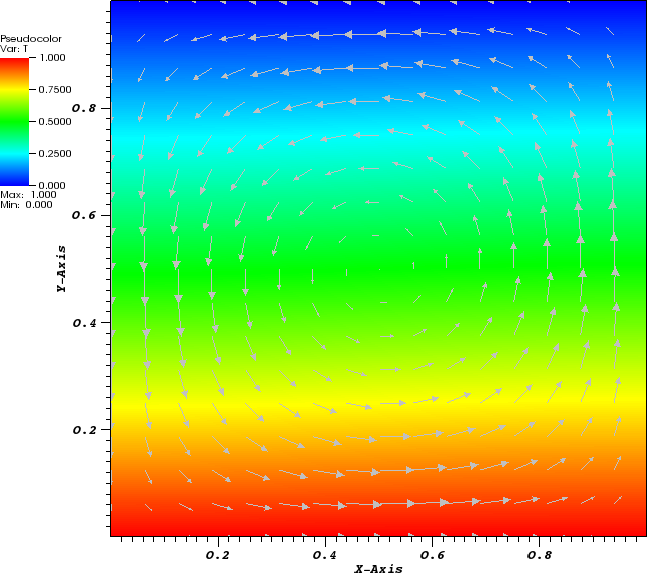
\includegraphics[width=0.4\textwidth]{cookbooks/convection-box/visit0000}
\hfill
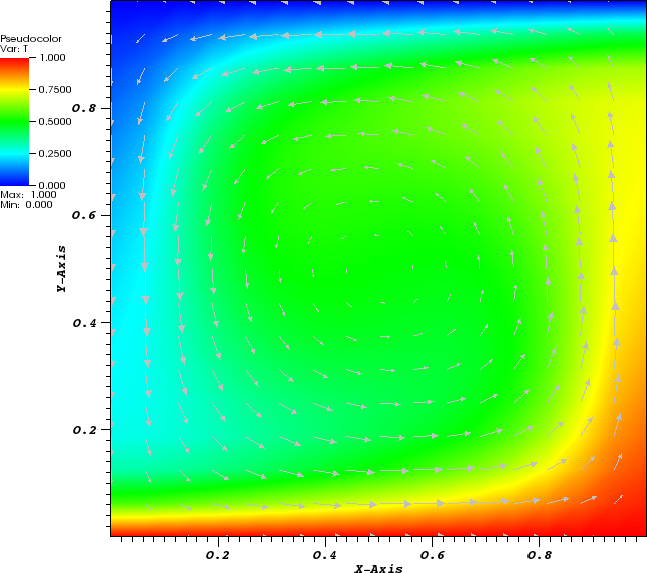
\includegraphics[width=0.4\textwidth]{cookbooks/convection-box/visit0001}
\hfill
\phantom.
\caption{\it Convection in a box: Initial temperature and velocity field (left)
and final state (right).}
\label{fig:convection-box-fields}
\end{figure}

There are many other things we can learn from the output files generated by
\aspect{}, specifically from the statistics file that contains information
collected at every time step and that has been discussed in
Section~\ref{sec:viz-stat}. In particular, in our input file, we have selected
that we would like to compute velocity, temperature, and heat flux statistics.
These statistics, among others, are listed in the statistics file whose head
looks like this for the current input file:
\begin{lstlisting}[frame=single,language=prmfile]
# 1: Time step number
# 2: Time (seconds)
# 3: Number of mesh cells
# 4: Number of Stokes degrees of freedom
# 5: Number of temperature degrees of freedom
# 6: Iterations for temperature solver
# 7: Iterations for Stokes solver
# 8: Time step size (seconds)
# 9: RMS velocity (m/s)
# 10: Max. velocity (m/s)
# 11: Minimal temperature (K)
# 12: Average temperature (K)
# 13: Maximal temperature (K)
# 14: Average nondimensional temperature (K)
# 15: Outward heat flux through boundary with indicator 0 (W)
# 16: Outward heat flux through boundary with indicator 1 (W)
# 17: Outward heat flux through boundary with indicator 2 (W)
# 18: Outward heat flux through boundary with indicator 3 (W)
# 19: Visualization file name
... lots of numbers arranged in columns ...
\end{lstlisting}

Fig.~\ref{fig:convection-box-stats} shows the results of visualizing the data
that can be found in columns 2 (the time) plotted against columns 9 and 10
(root mean square and maximal velocities). Plots of this kind can be generated with
\texttt{Gnuplot} by typing (see Section~\ref{sec:viz-stat} for a more thorough
discussion):
\begin{verbatim}
  plot "output/statistics" using 2:9 with lines
\end{verbatim}
Fig.~\ref{fig:convection-box-stats} shows clearly that the simulation
enters a steady state after about $t\approx 0.1$ and then changes very little. This can also be observed using the
graphical output files from which we have generated
Fig.~\ref{fig:convection-box-fields}. One can look further into this data to
find that the flux through the top and bottom boundaries is not exactly the same
(up to the obvious difference in sign, given that at the bottom boundary heat
flows into the domain and at the top boundary out of it) at the beginning of the
simulation until the fluid has attained its equilibrium. However, after
$t\approx 0.2$, the fluxes differ by only $5\cdot 10^{-5}$, i.e., by less than
0.001\% of their magnitude.%
\footnote{This difference is far smaller than the numerical error in the heat
flux on the mesh this data is computed on.}
The flux we get at the last time step, 4.931, is less than 1\% away from the
value reported in \cite{BBC89} although we compute on a $16\times 16$ mesh and
the values reported by Blankenbach are extrapolated from meshes of size up to
$72\times 72$. This shows the accuracy that can be obtained using a higher order
finite element. Secondly, the fluxes through the left and right boundary are not
exactly zero but small. Of course, we have prescribed boundary conditions of the
form $\frac{\partial T}{\partial \mathbf n}=0$ along these boundaries, but this
is subject to discretization errors. It is easy to verify that the heat flux
through these two boundaries disappears as we refine the mesh further.

\begin{figure}
\phantom.
\hfill
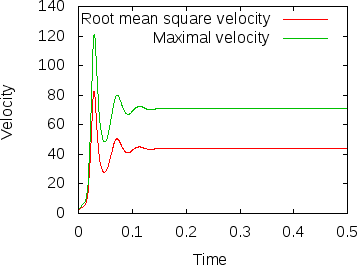
\includegraphics[width=0.4\textwidth]{cookbooks/convection-box/velocity}
\hfill
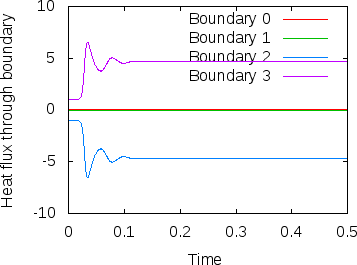
\includegraphics[width=0.4\textwidth]{cookbooks/convection-box/heatflux}
\hfill
\phantom.
\caption{\it Convection in a box: Root mean square and maximal velocity as a
function of simulation time (left). Heat flux through the four boundaries of
the box (right).}
\label{fig:convection-box-stats}
\end{figure}


Furthermore, \aspect{} automatically also collects statistics about many of its
internal workings. Fig.~\ref{fig:convection-box-iterations} shows the number of
iterations required to solve the Stokes and temperature linear systems in each
time step. It is easy to see that these are more difficult to solve in the
beginning when the solution still changes significant from time step to time
step. However, after some time, the solution remains mostly the same and solvers
then only need 9 or 10 iterations for the temperature equation and 4 or 5
iterations for the Stokes equations because the starting guess for the linear
solver -- the previous time step's solution -- is already pretty good. If you
look at any of the more complex cookbooks, you will find that one needs many
more iterations to solve these equations.

\begin{figure}
\phantom.
\hfill
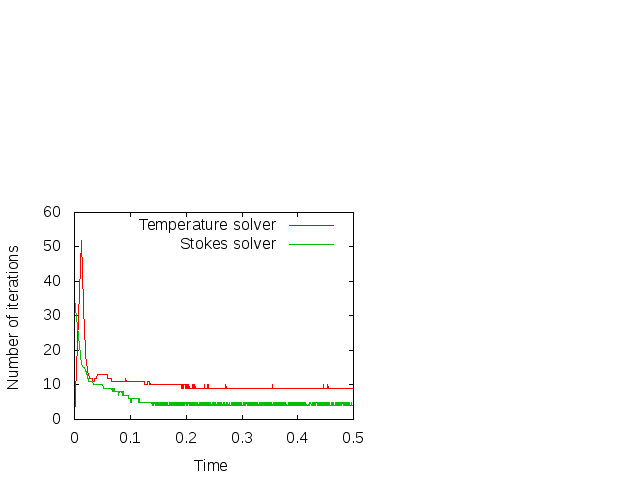
\includegraphics[width=0.4\textwidth]{cookbooks/convection-box/iterations}
\hfill
\phantom.
\caption{\it Convection in a box: Number of linear iterations required to solve
the Stokes and temperature equations in each time step.}
\label{fig:convection-box-iterations}
\end{figure}


\paragraph{Play time 1: Different Rayleigh numbers.} After showing you results
for the input file as it can be found in \url{cookbooks/convection-box.prm}, let us
end this section with a few ideas on how to play with it and what to explore.
The first direction one could take this example is certainly to consider
different Rayleigh numbers. As mentioned above, for the value $Ra=10^4$ for
which the results above have been produced, one gets a stable convection
pattern. On the other hand, for values $Ra<Ra_c\approx 780$, any movement of
the fluid dies down exponentially and we end up with a situation where the fluid
doesn't move and heat is transported from the bottom to the top only through
heat conduction. This can be explained by considering that the Rayleigh number
in a box of unit extent is defined as $Ra=\frac{g\alpha}{\eta k}$. A small
Rayleigh number means that the viscosity is too large (i.e., the buoyancy given
by the product of the magnitude of gravity times the thermal expension
coefficient is not strong enough to overcome friction forces within the fluid).

On the other hand, if the Rayleigh number is large (i.e., the viscosity is
small or the buoyancy large) then the fluid develops an unsteady convection
period. As we consider fluids with larger and larger $Ra$, this pattern goes
through a sequence of period-doubling events until flow finally becomes chaotic.
The structures of the flow pattern also become smaller and smaller.

\begin{figure}
\phantom.
\hfill
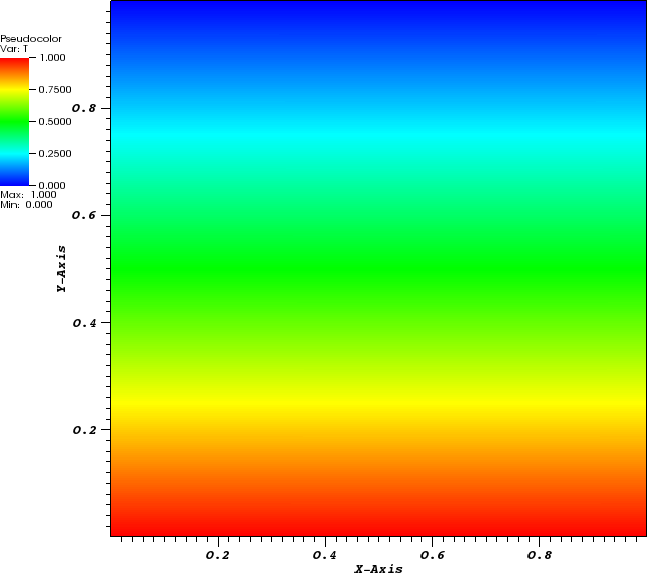
\includegraphics[width=0.4\textwidth]{cookbooks/convection-box/ra_1e2_visit0000}
\hfill
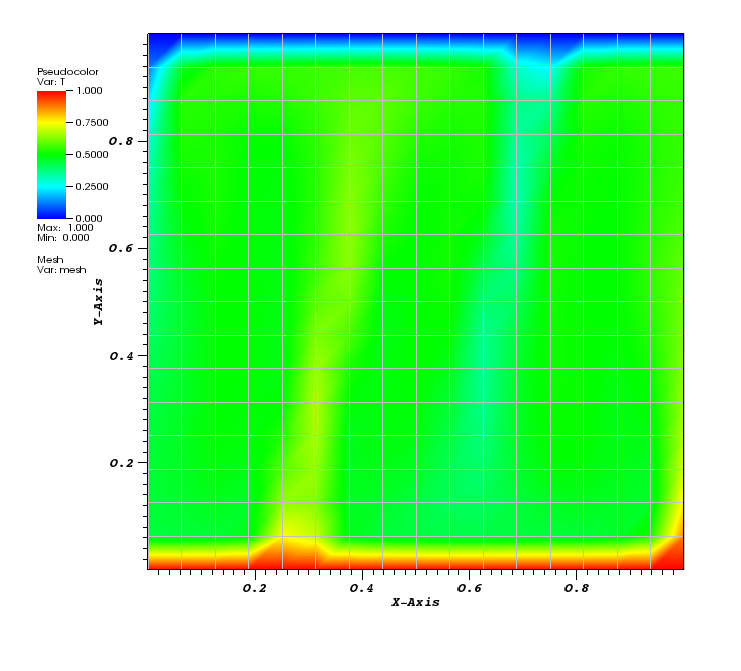
\includegraphics[width=0.4\textwidth]{cookbooks/convection-box/ra_1e6_visit0001}
\hfill
\phantom.
\caption{\it Convection in a box: Temperature fields at the end of a
simulation for $Ra=10^2$ where thermal diffusion dominates (left) and $Ra=10^6$
where convective heat transport dominates (right).
The mesh on the right is clearly too coarse to resolve the structure of the solution.}
\label{fig:convection-box-fields-different-Ra}
\end{figure}

\begin{figure}
\phantom.
\hfill
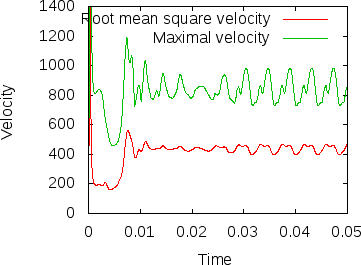
\includegraphics[width=0.4\textwidth]{cookbooks/convection-box/ra_1e6_velocity}
\hfill
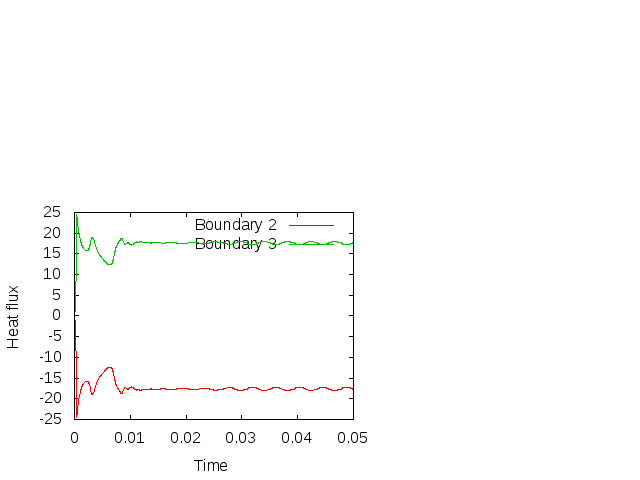
\includegraphics[width=0.4\textwidth]{cookbooks/convection-box/ra_1e6_heatflux}
\hfill
\phantom.
\caption{\it Convection in a box: Velocities (left) and heat flux across the
top and bottom boundaries (right) as a function of time at $Ra=10^6$.}
\label{fig:convection-box-stats-different-Ra}
\end{figure}

We illustrate these situations in
Fig.s~\ref{fig:convection-box-fields-different-Ra} and
\ref{fig:convection-box-stats-different-Ra}. The first shows the temperature
field at the end of a simulation for $Ra=10^2$ (below $Ra_c$) and at $Ra=10^6$.
Obviously, for the right picture, the mesh is not fine enough to accurately
resolve the features of the flow field and we would have to refine it more. The
second of the figures shows the velocity and heatflux statistics for the
computation with $Ra=10^6$; it is obvious here that the flow no longer settles
into a steady state but has a periodic behavior. This can also be seen by
looking at movies of the solution.

To generate these results, remember that we have chosen $\alpha=10^{-10}$ and
$g=10^{10}Ra$ in our input file. In other words, changing the input file to
contain the parameter setting
\begin{lstlisting}[frame=single,language=prmfile,escapechar=\%]
subsection Gravity model
  subsection Vertical
    set Magnitude = 1e16   # = Ra / Thermal expansion coefficient % \index[prmindex]{Magnitude} \index[prmindexfull]{Gravity model!Vertical!Magnitude} %
  end
end
\end{lstlisting}
will achieve the desired effect of computing with $Ra=10^6$.


\paragraph{Play time 2: Thinking about finer meshes.}
In our computations for $Ra=10^4$ we used a $16\times 16$ mesh and obtained a
value for the heat flux that differed from the generally accepted value from
Blankenbach \textit{et al.} \cite{BBC89} by less than 1\%. However, it may be
interesting to think about computing even more accurately. This is easily done
by using a finer mesh, for example. In the parameter file above, we have chosen
the mesh setting as follows:
\begin{lstlisting}[frame=single,language=prmfile,escapechar=\%]
subsection Mesh refinement
  set Initial global refinement                = 4 % \index[prmindex]{Initial global refinement} \index[prmindexfull]{Mesh refinement!Initial global refinement} %
  set Initial adaptive refinement              = 0 % \index[prmindex]{Initial adaptive refinement} \index[prmindexfull]{Mesh refinement!Initial adaptive refinement} %
  set Time steps between mesh refinement       = 0 % \index[prmindex]{Time steps between mesh refinement} \index[prmindexfull]{Mesh refinement!Time steps between mesh refinement} %
end
\end{lstlisting}
We start out with a box geometry consisting of a single cell that is refined
four times. Each time we split each cell into its 4 children, obtaining the
$16\times 16$ mesh already mentioned. The other settings indicate that we do not
want to refine the mesh adaptively at all in the first time step, and a setting
of zero for the last parameter means that we also never want to adapt the mesh
again at a later time. Let us stick with the never-changing, globally refined
mesh for now (we will come back to adaptive mesh refinement again at a later
time) and only vary the initial global refinement. In particular, we could
choose the parameter \texttt{Initial global refinement} to be 5, 6, or even
larger. This will get us closer to the exact solution albeit at the expense of a
significantly increased computational time.

A better strategy is to realize that for $Ra=10^4$, the flow enters a steady
state after settling in during the first part of the simulation (see, for
example, the graphs in Fig.~\ref{fig:convection-box-stats}). Since we are not
particularly interested in this initial transient process, there is really no
reason to spend CPU time using a fine mesh and correspondingly small time
steps during this part of the simulation (remember that each refinement results
in four times as many cells in 2d and a time step half as long, making reaching
a particular time at least 8 times as expensive, assuming that all solvers in
\aspect{} scale perfectly with the number of cells). Rather, we can use a
parameter in the \aspect{} input file that let's us increase the mesh resolution
at later times. To this end, let us use the following snippet for the input
file:
\begin{lstlisting}[frame=single,language=prmfile,escapechar=\%]
subsection Mesh refinement
  set Initial global refinement                = 3 % \index[prmindex]{Initial global refinement} \index[prmindexfull]{Mesh refinement!Initial global refinement} %
  set Initial adaptive refinement              = 0 % \index[prmindex]{Initial adaptive refinement} \index[prmindexfull]{Mesh refinement!Initial adaptive refinement} %
  set Time steps between mesh refinement       = 0 % \index[prmindex]{Time steps between mesh refinement} \index[prmindexfull]{Mesh refinement!Time steps between mesh refinement} %
  set Additional refinement times              = 0.2, 0.3, 0.4 % \index[prmindex]{Additional refinement times} \index[prmindexfull]{Mesh refinement!Additional refinement times} %
  set Refinement fraction                      = 1.0 % \index[prmindex]{Refinement fraction} \index[prmindexfull]{Mesh refinement!Refinement fraction} %
  set Coarsening fraction                      = 0.0 % \index[prmindex]{Coarsening fraction} \index[prmindexfull]{Mesh refinement!Coarsening fraction} %
end
\end{lstlisting}

What this does is the following: We start with an $8\times 8$ mesh (3 times
globally refined) but then at times $t=0.2,0.3$ and $0.4$ we refine the mesh
using the default refinement indicator (which one this is is not important
because of the next statement). Each time, we refine, we refine a fraction 1.0
of the cells, i.e., \textit{all} cells and we coarsen a fraction of 0.0 of the
cells, i.e. no cells at all. In effect, at these additional refinement times, we
do another global refinement, bringing us to refinement levels 4, 5 and finally
6.

\begin{figure}
\phantom.
\hfill
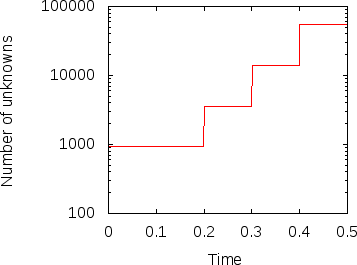
\includegraphics[width=0.4\textwidth]{cookbooks/convection-box/steps_unknowns}
\hfill
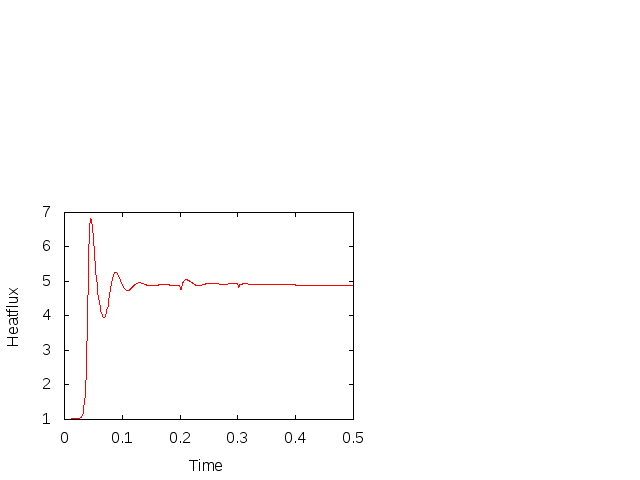
\includegraphics[width=0.4\textwidth]{cookbooks/convection-box/steps_heatflux}
\hfill
\phantom.
\caption{\it Convection in a box: Refinement in stages. Total number
of unknowns in each time step, including all velocity, pressure and
temperature unknowns (left) and heat flux across the top boundary (right).}
\label{fig:convection-box-stats-steps}
\end{figure}


Fig.~\ref{fig:convection-box-stats-steps} shows the results. In the left panel,
we see how the number of unknowns grows over time (note the logscale for the
$y$-axis). The right panel displays the heat flux. The jumps in the number of
cells is clearly visible in this picture as well. This may be surprising at
first but remember that the mesh is clearly too coarse in the beginning to
really resolve the flow and so we should expect that the solution changes
significantly if the mesh is refined. This effect becomes smaller with every
additional refinement and is barely visible at the last time this happens,
indicating that the mesh before this refinement step may already have been fine
enough to resolve the majority of the dynamics.

In any case, we can compare the heat fluxes we obtain at the end of these
computations: With a globally four times refined mesh, we get a value of 4.931
(an error of approximately 1\% against the accepted value from Blankenbach,
$4.884409\pm 0.00001$). With a globally five times refined mesh we get 4.914 (an
error of 0.6\%) and with the mesh generated using the procedure above we get
4.895 with the four digits printed on the screen%
\footnote{The statistics file gives this
value to more digits: 4.89488768. However, these are clearly more digits than
the result is accurate.}
(corresponding to an error of 0.2\%). In other words, our
simple procedure of refining the mesh during the simulation run yields an
accuracy of three times smaller than using the globally refined approach even
though the compute time is not much larger than that necessary for the 5 times
globally refined mesh.


\paragraph{Play time 3: Changing the finite element in use.}
Another way to increase the accuracy of a finite element computation is to use a
higher polynomial degree for the finite element shape functions. By default,
\aspect{} uses quadratic shape functions for the velocity and the temperature
and linear ones for the pressure. However, this can be changed with a single
number in the input file.

Before doing so, let us consider some aspects of such a change. First, looking
at the pictures of the solution in Fig.~\ref{fig:convection-box-fields}, one
could surmise that the quadratic elements should be able to resolve the velocity
field reasonably well given that it is rather smooth. On the other hand, the
temperature field has a boundary layer at the top and bottom. One could
conjecture that the temperature polynomial degree is therefore the limiting
factor and not the polynomial degree for the flow variables. We will test this
conjecture below. Secondly, given the nature of the equations, increasing the
polynomial degree of the flow variables increases the cost to solve these
equations by a factor of $\frac{22}{9}$ in 2d (you can get this factor by
counting the number of degrees of freedom uniquely associated with each cell) but leaves
the time step size and the cost of solving the temperature system unchanged. On
the other hand, increasing the polynomial degree of the temperature variable
from 2 to 3 requires $\frac 94$ times as many degrees of freedom for the
temperature and also requires us to reduce the size of the time step by a factor
of $\frac 23$. Because solving the temperature system is not a dominant factor
in each time step (see the timing results shown at the end of the screen output
above), the reduction in time step is the only important factor. Overall,
increasing the polynomial degree of the temperature variable turns out to be the
cheaper of the two options.

Following these considerations, let us add the following section to the
parameter file:
\begin{lstlisting}[frame=single,language=prmfile,escapechar=\%]
subsection Discretization
  set Stokes velocity polynomial degree       = 2 % \index[prmindex]{Stokes velocity polynomial degree} \index[prmindexfull]{Discretization!Stokes velocity polynomial degree} %
  set Temperature polynomial degree           = 3 % \index[prmindex]{Temperature polynomial degree} \index[prmindexfull]{Discretization!Temperature polynomial degree} %
end
\end{lstlisting}
This leaves the velocity and pressure shape functions at quadratic and linear
polynomial degree but increases the polynomial degree of the temperature from
quadratic to cubic. Using the original, four times globally refined mesh, we
then get the following output:
\begin{lstlisting}[frame=single,language=ksh]
Number of active cells: 256 (on 5 levels)
Number of degrees of freedom: 4,868 (2,178+289+2,401)

*** Timestep 0:  t=0 seconds
   Solving temperature system... 0 iterations.
   Rebuilding Stokes preconditioner...
   Solving Stokes system... 30+5 iterations.

[... ...]

*** Timestep 1619:  t=0.499807 seconds
   Solving temperature system... 8 iterations.
   Solving Stokes system... 5 iterations.

   Postprocessing:
     RMS, max velocity:                  42.9 m/s, 69.5 m/s
     Temperature min/avg/max:            0 K, 0.5 K, 1 K
     Heat fluxes through boundary parts: -0.004622 W, 0.004624 W, -4.878 W, 4.878 W


+---------------------------------------------+------------+------------+
| Total wallclock time elapsed since start    |       127s |            |
|                                             |            |            |
| Section                         | no. calls |  wall time | % of total |
+---------------------------------+-----------+------------+------------+
| Assemble Stokes system          |      1620 |      3.03s |       2.4% |
| Assemble temperature system     |      1620 |      75.7s |        60% |
| Build Stokes preconditioner     |         1 |    0.0422s |     0.033% |
| Build temperature preconditioner|      1620 |      21.7s |        17% |
| Solve Stokes system             |      1620 |      10.3s |       8.1% |
| Solve temperature system        |      1620 |       4.9s |       3.8% |
| Initialization                  |         2 |    0.0246s |     0.019% |
| Postprocessing                  |      1620 |      8.05s |       6.3% |
| Setup dof systems               |         1 |    0.0438s |     0.034% |
+---------------------------------+-----------+------------+------------+
\end{lstlisting}

Note here that the heat flux through the top and bottom boundaries is now
computed as 4.878, an error of 0.13\%. This is 4 times more accurate than the
once more globally refined mesh with the original quadratic elements, at a cost
significantly smaller. Furthermore, we can of course combine this with the mesh
that is gradually refined as simulation time progresses, and we then get a heat
flux that is equal to 4.8843, only 0.002\% away from the accepted value!

As a final remark, to test our hypothesis that it was indeed the temperature
polynomial degree that was the limiting factor, we can increase the Stokes
polynomial degree to 3 while leaving the temperature polynomial degree at 2. A
quick computation shows that in that case we get a heat flux of 4.931 -- exactly
the same value as we got initially with the lower order Stokes element. In other
words, at least for this testcase, it really was the temperature variable that
limits the accuracy.


\subsubsection{Convection in a box with prescribed, variable velocity boundary conditions}

A similarly simple setup is to equip the model we had in the previous section
with a different set of boundary conditions. There, we used slip boundary
conditions, i.e., the fluid can flow tangentially along the four sides of our
box but this tangential velocity is unspecified. On the other hand, in many
situations, one would like to actually prescribe the tangential flow velocity as
well. A typical application would be to use boundary conditions at the top that
describe experimentally determined velocities of plates. This cookbook shows a
simple version of something like this. To make it slightly more interesting, we
choose a $2\times 1$ domain in 2d.

Like for many other things, \aspect{} has a set of plugins for prescribed
velocity boundary values (see
Sections~\ref{parameters:Boundary_20velocity_20model} and
\ref{sec:prescribed-velocity-boundary-conditions}). These plugins allow one to
write sophisticated models for the boundary velocity on parts or all of the
boundary, but there is also one simple implementation that just takes a formula
for the components of the velocity.

To illustrate this, let us consider the \url{cookbooks/platelike-boundary.prm}
input file. It essentially extends the input file considered in the previous example.
The part of this file that we are particularly interested in in the current
context is the selection of the kind of boundary conditions on the four
sides of the box geometry, which we do using a section like this:
\begin{lstlisting}[frame=single,language=prmfile,escapechar=\%]
subsection Model settings
  set Fixed temperature boundary indicators   = 2, 3 % \index[prmindex]{Fixed temperature boundary indicators} \index[prmindexfull]{Model settings!Fixed temperature boundary indicators} %
  set Zero velocity boundary indicators       =  % \index[prmindex]{Zero velocity boundary indicators} \index[prmindexfull]{Model settings!Zero velocity boundary indicators} %
  set Tangential velocity boundary indicators = 0, 1, 2 % \index[prmindex]{Tangential velocity boundary indicators} \index[prmindexfull]{Model settings!Tangential velocity boundary indicators} %
  set Prescribed velocity boundary indicators = 3: function % \index[prmindex]{Prescribed velocity boundary indicators} \index[prmindexfull]{Model settings!Prescribed velocity boundary indicators} %
end
\end{lstlisting}

Following the convention for numbering boundaries described in the previous
section, this means that we prescribe a fixed temperature at the bottom and top sides of the box (boundary
numbers two and three). We use tangential flow at boundaries zero, one and two
(left, right and bottom).
Finally, the last entry above is a comma separated list (here with only a single element) of pairs consisting of the
number of a boundary and the name of the prescribed velocity boundary model to
be used on this boundary. Here, we use the \texttt{function} boundary model,
which allows us to provide a function-like notation for the components of the
velocity vector at the boundary.

The second part we need is that we actually describe the function that sets the
velocity. We do this as follows:
\begin{lstlisting}[frame=single,language=prmfile,escapechar=\%]
subsection Boundary velocity model
  subsection Function
    set Variable names      = x,z,t % \index[prmindex]{Variable names} \index[prmindexfull]{Boundary velocity model!Function!Variable names} %
    set Function constants  = pi=3.1415926 % \index[prmindex]{Function constants} \index[prmindexfull]{Boundary velocity model!Function!Function constants} %
    set Function expression = if(x>1+sin(0.5*pi*t), 1, -1); 0 % \index[prmindex]{Function expression} \index[prmindexfull]{Boundary velocity model!Function!Function expression} %
  end
end
\end{lstlisting}
The first of these gives names to the components of the position vector (here,
we are in 2d and we use $x$ and $z$ as spatial variable names) and the time.
We could have left this entry at its default, \texttt{x,y,t}, but since we
often think in terms of ``depth'' as the vertical direction, let us use
\texttt{z} for the second coordinate.
In the second parameter we define symbolic constants that can be used
in the formula for the velocity that is specified in the last parameter. This
formula needs to have as many components as there are space dimensions,
separated by semicolons. As stated, this means that we prescribe the
(horizontal) $x$-velocity and set the vertical velocity to zero. The horizontal
component is here either $1$ or $-1$, depending on whether we are to the right
or the left of the point $1+\sin(\pi t/2)$ that is moving back and forth with
time once every four time units. The \texttt{if} statement understood by the
parser we use for these formulas has the syntax
\texttt{if(condition, value-if-true, value-if-false)}.

\note{While you can enter most any expression into the parser for these
velocity boundary conditions, not all make sense. In particular, if you use an
incompressible medium like we do here, then you need to make sure that either
the flow you prescribe is indeed tangential, or that at least the flow into and
out of the boundary this function applies to is balanced so that in sum the
amount of material in the domain stays constant.

It is in general not possible for \aspect{} to verify that a given input is
sensible. However, you will quickly find out if it isn't: The linear solver for
the Stokes equations will simply not converge. For example, if your function
expression in the input file above read \\
\hspace*{.25cm} \texttt{if(x>1+sin(0.5*pi*t), 1, -1); 1}\\
then at the time of writing this you would get the following error message: \\
\hspace*{.25cm}\texttt{*** Timestep 0:  t=0 seconds} \\
\hspace*{.25cm}\texttt{   Solving temperature system... 0 iterations.} \\
\hspace*{.25cm}\texttt{   Rebuilding Stokes preconditioner...} \\
\hspace*{.25cm}\texttt{   Solving Stokes system... } \\
\\
\hspace*{.25cm}\texttt{\ldots some timing output \ldots} \\
\\
\\
\hspace*{.25cm}\texttt{----------------------------------------------------} \\
\hspace*{.25cm}\texttt{Exception on processing: } \\
\hspace*{.25cm}\texttt{Iterative method reported convergence failure in step
9539 with residual 6.0552} \\
\hspace*{.25cm}\texttt{Aborting!} \\
\hspace*{.25cm}\texttt{----------------------------------------------------}

The reason is, of course, that there is no incompressible (divergence free) flow
field that allows for a constant vertical outflow component along the top
boundary without corresponding inflow anywhere else.}

The remainder of the setup is described in the following, complete input file:
\begin{lstlisting}[frame=single,language=prmfile,escapechar=\%]
############### Global parameters

set Dimension                              = 2 % \index[prmindex]{Dimension} \index[prmindexfull]{Dimension} %
set Start time                             = 0 % \index[prmindex]{Start time} \index[prmindexfull]{Start time} %
set End time                               = 20 % \index[prmindex]{End time} \index[prmindexfull]{End time} %
set Use years in output instead of seconds = false % \index[prmindex]{Use years in output instead of seconds} \index[prmindexfull]{Use years in output instead of seconds} %
set Output directory                       = output % \index[prmindex]{Output directory} \index[prmindexfull]{Output directory} %


############### Parameters describing the model
# Let us here choose again a box domain of size 2x1
# where we fix the temperature at the bottom and top,
# allow free slip along the bottom, left and right,
# and prescribe the velocity along the top using the
# `function' description.

subsection Geometry model
  set Model name = box % \index[prmindex]{Model name} \index[prmindexfull]{Geometry model!Model name} %

  subsection Box
    set X extent = 2 % \index[prmindex]{X extent} \index[prmindexfull]{Geometry model!Box!X extent} %
    set Y extent = 1 % \index[prmindex]{Y extent} \index[prmindexfull]{Geometry model!Box!Y extent} %
  end
end


subsection Model settings
  set Fixed temperature boundary indicators   = 2, 3 % \index[prmindex]{Fixed temperature boundary indicators} \index[prmindexfull]{Model settings!Fixed temperature boundary indicators} %
  set Zero velocity boundary indicators       =  % \index[prmindex]{Zero velocity boundary indicators} \index[prmindexfull]{Model settings!Zero velocity boundary indicators} %
  set Tangential velocity boundary indicators = 0, 1, 2 % \index[prmindex]{Tangential velocity boundary indicators} \index[prmindexfull]{Model settings!Tangential velocity boundary indicators} %
  set Prescribed velocity boundary indicators = 3: function % \index[prmindex]{Prescribed velocity boundary indicators} \index[prmindexfull]{Model settings!Prescribed velocity boundary indicators} %
end


# We then set the temperature to one at the bottom and zero
# at the top:
subsection Boundary temperature model
  set Model name = box % \index[prmindex]{Model name} \index[prmindexfull]{Boundary temperature model!Model name} %

  subsection Box
    set Bottom temperature = 1 % \index[prmindex]{Bottom temperature} \index[prmindexfull]{Boundary temperature model!Box!Bottom temperature} %
    set Top temperature    = 0 % \index[prmindex]{Top temperature} \index[prmindexfull]{Boundary temperature model!Box!Top temperature} %
  end
end


# The velocity along the top boundary models a spreading
# center that is moving left and right:
subsection Boundary velocity model
  subsection Function
    set Variable names      = x,z,t % \index[prmindex]{Variable names} \index[prmindexfull]{Boundary velocity model!Function!Variable names} %
    set Function constants  = pi=3.1415926 % \index[prmindex]{Function constants} \index[prmindexfull]{Boundary velocity model!Function!Function constants} %
    set Function expression = if(x>1+sin(0.5*pi*t), 1, -1); 0 % \index[prmindex]{Function expression} \index[prmindexfull]{Boundary velocity model!Function!Function expression} %
  end
end


# We then choose a vertical gravity model and describe the
# initial temperature with a vertical gradient. The default
# strength for gravity is one. The material model is the
# same as before.
subsection Gravity model
  set Model name = vertical % \index[prmindex]{Model name} \index[prmindexfull]{Gravity model!Model name} %
end


subsection Initial conditions
  set Model name = function % \index[prmindex]{Model name} \index[prmindexfull]{Initial conditions!Model name} %

  subsection Function
    set Variable names      = x,z % \index[prmindex]{Variable names} \index[prmindexfull]{Initial conditions!Function!Variable names} %
    set Function expression = (1-z)     % \index[prmindex]{Function expression} \index[prmindexfull]{Initial conditions!Function!Function expression} %
  end
end


subsection Material model
  set Model name = simple % \index[prmindex]{Model name} \index[prmindexfull]{Material model!Model name} %

  subsection Simple model
    set Thermal conductivity          = 1e-6 % \index[prmindex]{Thermal conductivity} \index[prmindexfull]{Material model!Simple model!Thermal conductivity} %
    set Thermal expansion coefficient = 1e-4 % \index[prmindex]{Thermal expansion coefficient} \index[prmindexfull]{Material model!Simple model!Thermal expansion coefficient} %
    set Viscosity                     = 1 % \index[prmindex]{Viscosity} \index[prmindexfull]{Material model!Simple model!Viscosity} %
  end
end


# The final part of this input file describes how many times the
# mesh is refined and what to do with the solution once computed
subsection Mesh refinement
  set Initial adaptive refinement        = 0 % \index[prmindex]{Initial adaptive refinement} \index[prmindexfull]{Mesh refinement!Initial adaptive refinement} %
  set Initial global refinement          = 5 % \index[prmindex]{Initial global refinement} \index[prmindexfull]{Mesh refinement!Initial global refinement} %
  set Time steps between mesh refinement = 0 % \index[prmindex]{Time steps between mesh refinement} \index[prmindexfull]{Mesh refinement!Time steps between mesh refinement} %
end


subsection Postprocess
  set List of postprocessors = visualization, temperature statistics, heat flux statistics % \index[prmindex]{List of postprocessors} \index[prmindexfull]{Postprocess!List of postprocessors} %

  subsection Visualization
    set Time between graphical output = 0.1 % \index[prmindex]{Time between graphical output} \index[prmindexfull]{Postprocess!Visualization!Time between graphical output} %
  end
end
\end{lstlisting}

This model description yields a setup with a Rayleigh number of 200 (taking
into account that the domain has size 2). It would, thus, be dominated by heat
conduction rather than convection if the prescribed velocity boundary conditions
did not provide a stirring action. Visualizing the results of this simulation%
\footnote{In fact, the pictures are generated using a twice more refined mesh
to provide adequate resolution. We keep the default setting of five
global refinements in the parameter file as documented above to keep compute
time reasonable when using the default settings.}
yields images like the ones shown in Fig.~\ref{fig:platelike}.

\begin{figure}
  \centering
  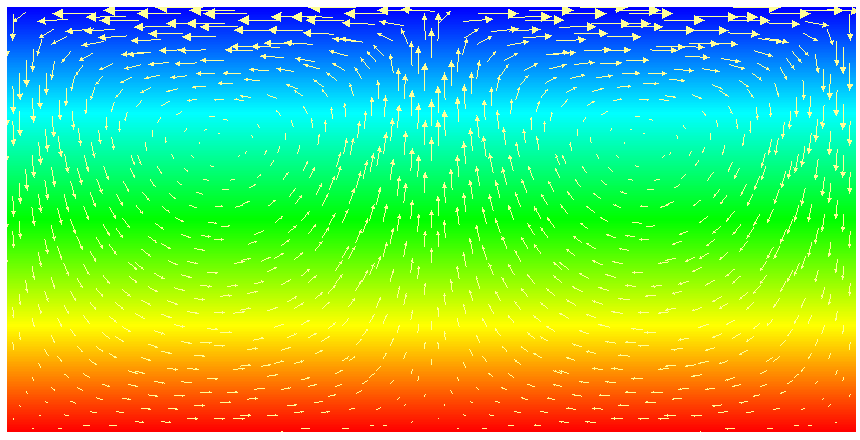
\includegraphics[width=0.3\textwidth]{cookbooks/platelike-boundary/visit0000.png}
  \hfill
  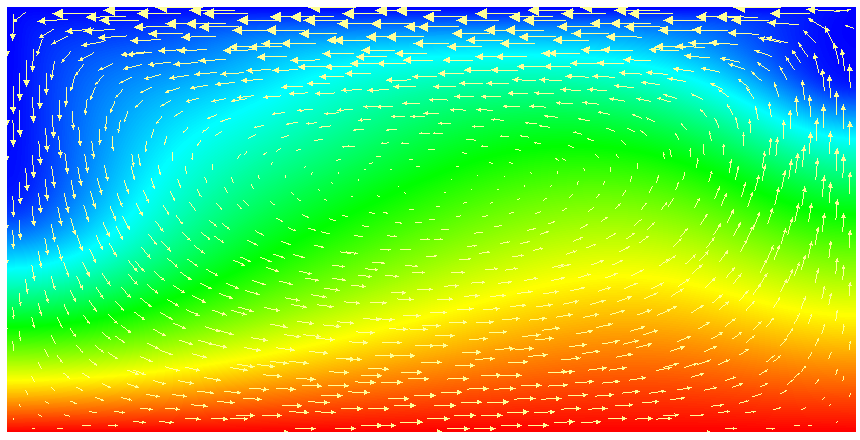
\includegraphics[width=0.3\textwidth]{cookbooks/platelike-boundary/visit0001.png}
  \hfill
  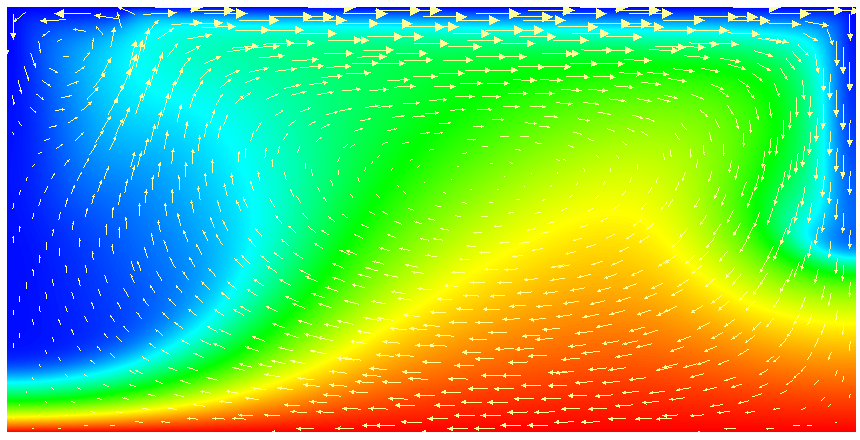
\includegraphics[width=0.3\textwidth]{cookbooks/platelike-boundary/visit0003.png}
  \\
  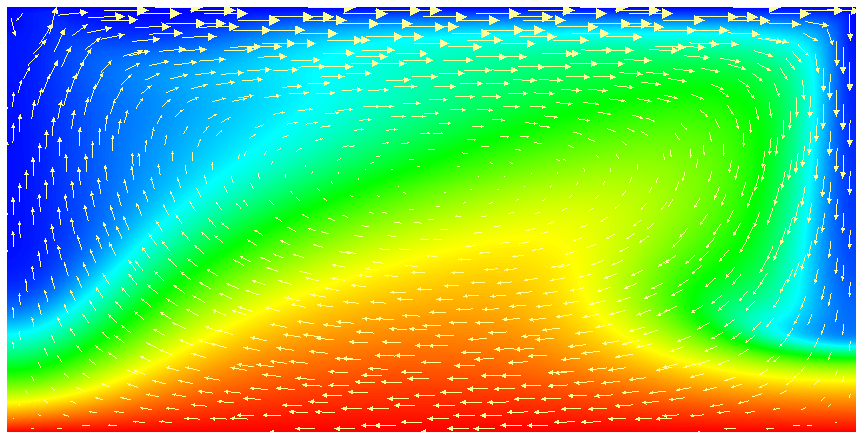
\includegraphics[width=0.3\textwidth]{cookbooks/platelike-boundary/visit0004.png}
  \hfill
  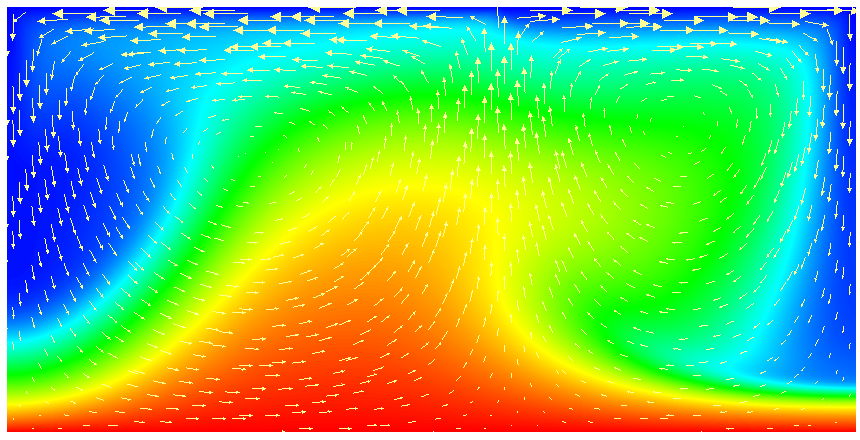
\includegraphics[width=0.3\textwidth]{cookbooks/platelike-boundary/visit0005.png}
  \hfill
  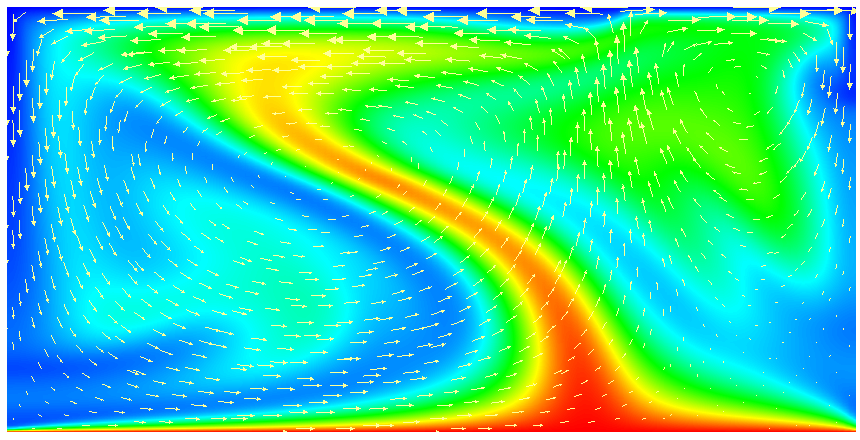
\includegraphics[width=0.3\textwidth]{cookbooks/platelike-boundary/visit0006.png}
  \caption{Variable velocity boundary conditions: Temperature and velocity
  fields at the initial time (top left) and at various other points in time during the
  simulation.}
  \label{fig:platelike}
\end{figure}


\subsubsection{Using passive and active compositional fields}
\label{sec:cookbooks-composition}

One frequently wants to track where material goes, either because one simply
wants to see where stuff ends up (e.g., to determine if a particular model
yields mixing between the lower and upper mantle) or because the material model
in fact depends not only pressure, temperature and location but also on the
mass fractions of certain chemical or other species. We will refer to the first
case as \textit{passive} and the latter as \textit{active} to indicate the role
of the additional quantities whose distribution we want to track. We refer to
the whole process as \textit{compositional} since we consider quantities that
have the flavor of something that denotes the composition of the material at any
given point.

There are basically two ways to achieve this: one can advect a set of
particles (``tracers'') along with the velocity field, or one can advect along a
field. In the first case, where the closest particle came from indicates the
value of the concentration at any given position. In the latter case, the
concentration(s) at any given position is simply given by the value of the
field(s) at this location.

\aspect{} implements both strategies, at least to a certain degree. In this
cookbook, we will follow the route of advected fields.

\paragraph{The passive case.}
We will consider the
exact same situation as in the previous section but we will ask where the
material that started in the bottom 20\% of the domain
ends up, as well as the material that started in the top 20\%. For the moment,
let us assume that there is no material between the materials at the bottom, the
top, and the middle. The way to describe this situation is to simply add the
following block of definitions to the parameter file (you can find the full
parameter file in \url{cookbooks/compositional-passive.prm}:

\begin{lstlisting}[frame=single,language=prmfile,escapechar=\%]
# This is the new part: We declare that there will
# be two compositional fields that will be
# advected along. Their initial conditions are given by
# a function that is one for the lowermost 0.2 height
# units of the domain and zero otherwise in the first case,
# and one in the top most 0.2 height units in the latter.
subsection Compositional fields
  set Number of fields = 2
end

subsection Compositional initial conditions
  set Model name = function

  subsection Function
    set Variable names      = x,y
    set Function expression = if(y<0.2, 1, 0) ; if(y>0.8, 1, 0) % \index[prmindex]{Function expression} \index[prmindexfull]{Compositional initial conditions!Function!Function expression} %
  end
end
\end{lstlisting}

Running this simulation yields results such as the ones shown in
Fig.~\ref{fig:compositional-passive} where we show the values of the functions
$c_1(\mathbf x,t)$ and $c_2(\mathbf x,t)$ at various times in the simulation.
Because these fields were one only inside the lowermost and uppermost parts of
the domain, zero everywhere else, and because they have simply been advected
along with the flow field, the places where they are larger than one half
indicate where material has been transported to so far.%
\footnote{Of course, this interpretation suggests that we could have achieved
the same goal by encoding everything into a single function -- that would, for
example, have had initial values one, zero and minus one in the three parts of
the domain we are interested in.}

\begin{figure}
  \centering
  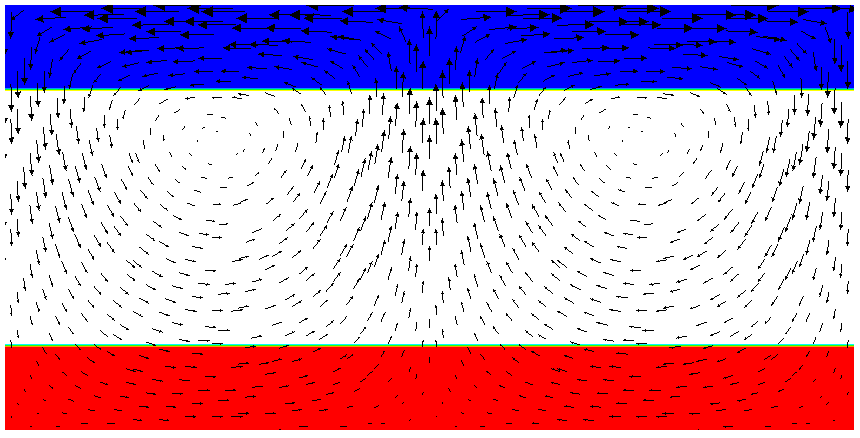
\includegraphics[width=0.3\textwidth]{cookbooks/composition-passive/visit0007.png}
  \hfill
  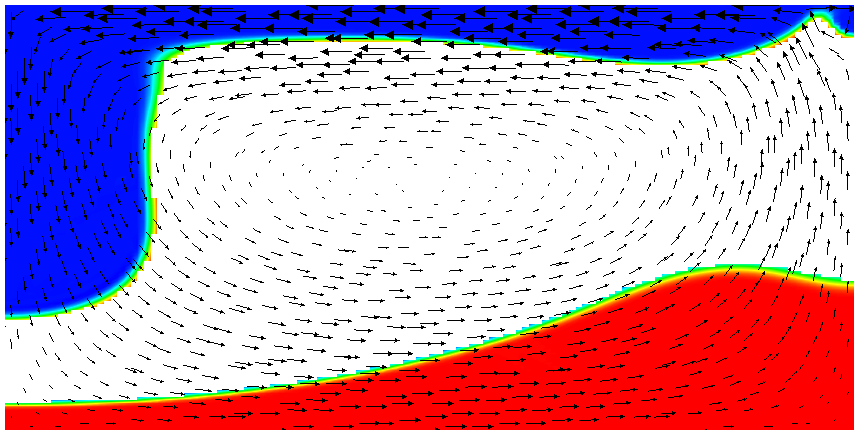
\includegraphics[width=0.3\textwidth]{cookbooks/composition-passive/visit0008.png}
  \hfill
  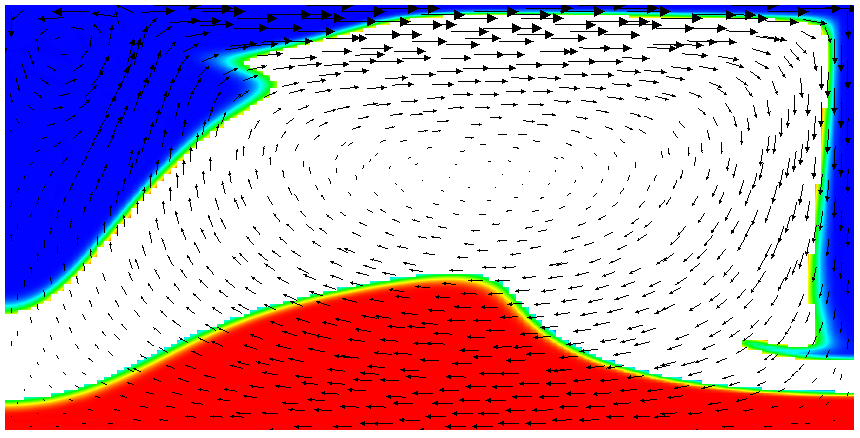
\includegraphics[width=0.3\textwidth]{cookbooks/composition-passive/visit0009.png}
  \\
  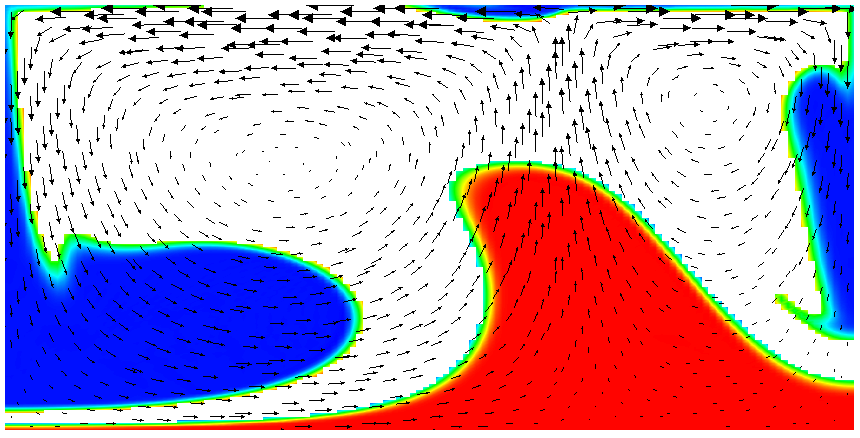
\includegraphics[width=0.3\textwidth]{cookbooks/composition-passive/visit0010.png}
  \hfill
  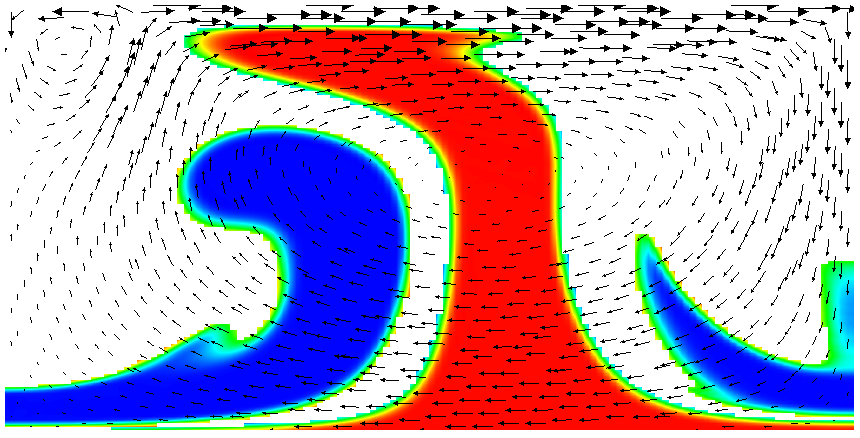
\includegraphics[width=0.3\textwidth]{cookbooks/composition-passive/visit0012.png}
  \hfill
  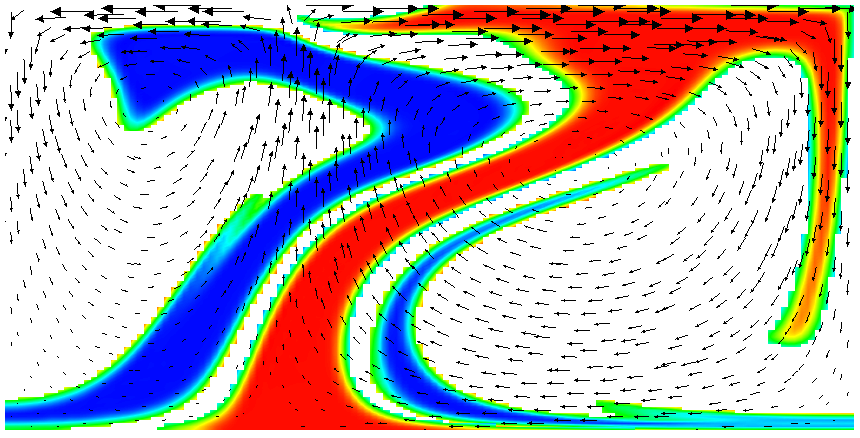
\includegraphics[width=0.3\textwidth]{cookbooks/composition-passive/visit0014.png}
  \caption{Passive compositional fields: The figures show, at
    different times in the simulation, the velocity field along with
    those locations where the first compositional field is larger than
    0.5 (in red, indicating the locations where material from the bottom
    of the domain has gone) as well as where the second compositional
    field is larger than 0.5 (in blue, indicating material from the top
    of the domain. The results were obtained with two more global
    refinement steps compared to the
    \url{cookbooks/compositional-passive.prm} input file.}
  \label{fig:compositional-passive}
\end{figure}

\begin{figure}
  \centering
  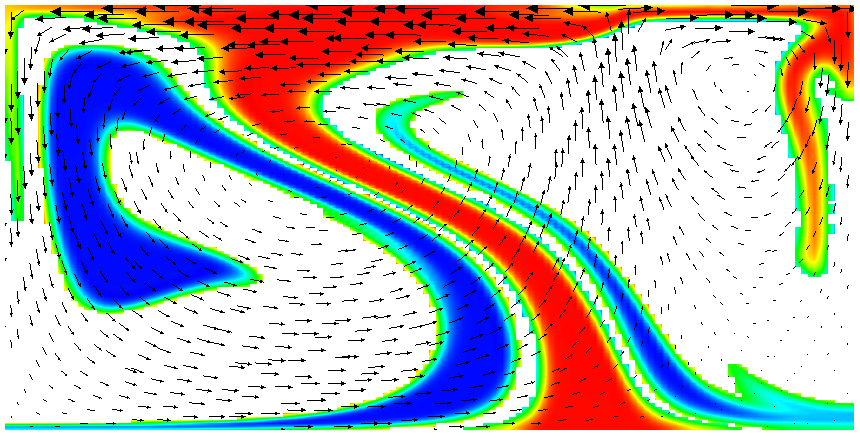
\includegraphics[height=0.3\textwidth]{cookbooks/composition-passive/visit0015.png}
  \hfill
  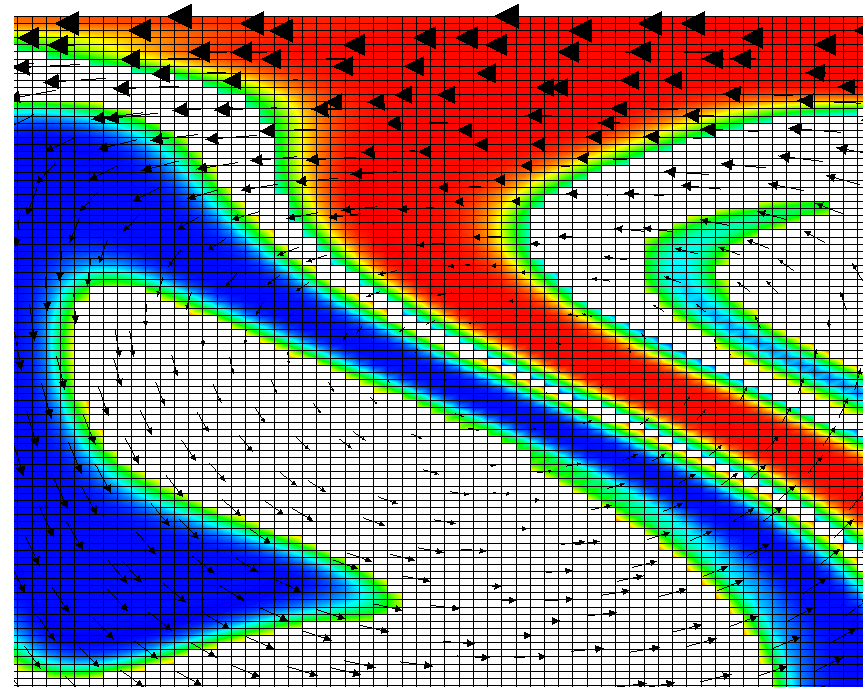
\includegraphics[height=0.3\textwidth]{cookbooks/composition-passive/visit0017.png}
  \caption{Passive compositional fields: A later image of the simulation
    corresponding to the sequence shown in
    Fig.~\ref{fig:compositional-passive} (left) and zoom-in on the
    center, also showing the mesh (right).}
  \label{fig:compositional-passive-zoom}
\end{figure}


Fig.~\ref{fig:compositional-passive} shows one aspect of compositional
fields that occasionally makes them difficult to use for very long
time computations. The simulation shown here runs for 20 time units,
where every cycle of the spreading center at the top moving left and
right takes 4 time units, for a total of 5 such cycles. While this is
certainly no short-term simulation, it is obviously visible in the
figure that the interface between the materials has diffused over
time. Fig.~\ref{fig:compositional-passive-zoom} shows a zoom into the
center of the domain at the final time of the simulation. The
figure only shows values that are larger than 0.5, and it looks like
the transition from red or blue to the edge of the shown region is no
wider than 3 cells. This means that the computation is not overly
diffusive but it is nevertheless true that this method has difficulty
following long and thin filaments.%
\footnote{We note that this is no different for tracers where the
  position of tracers has to be integrated over time and is subject to
  numerical error. In simulations, their location is therefore not the
  exact one but also subject to a diffusive process resulting from
  numerical inaccuracies. Furthermore, in long thin filaments, the
  number of tracers per cell often becomes too small and new tracers
  have to be inserted; their properties are then interpolated from the
  surrounding tracers, a process that also incurs a smoothing penalty.}
This is an area in which \aspect{} may see improvements in the future.


\begin{figure}
  \centering
  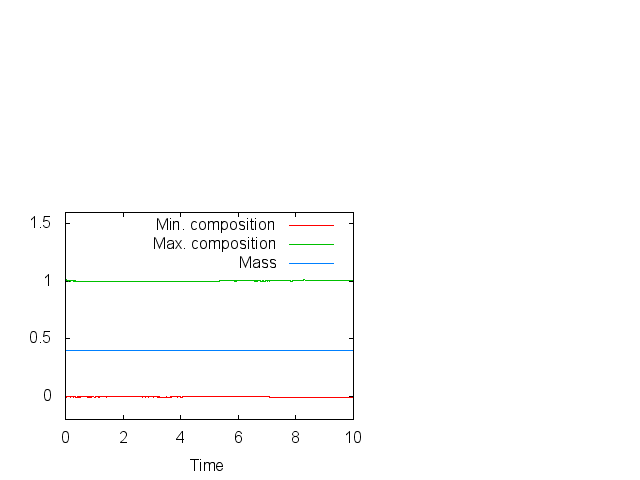
\includegraphics[width=0.4\textwidth]{cookbooks/composition-passive/mass-composition-1.png}
  \caption{Passive compositional fields: Minimum and maximum of the first compositional variable
   over time, as well as the mass $m_1(t)=\int_\Omega c_1(\mathbf x,t)$ stored in this variable.}
  \label{fig:compositional-passive-mass}
\end{figure}

A different way of looking at the quality of compositional fields as opposed to
tracers is to ask whether they conserve mass. In the current context, the
mass contained in the $i$th compositional field is $m_i(t)=\int_\Omega c_i(\mathbf x,t)$.
This can easily be achieve in the following way, by adding the \texttt{composition statistics}
postprocessor:
\begin{lstlisting}[frame=single,language=prmfile,escapechar=\%]
subsection Postprocess
  set List of postprocessors = visualization, temperature statistics, composition statistics % \index[prmindex]{List of postprocessors} \index[prmindexfull]{Postprocess!List of postprocessors} %
end
\end{lstlisting}
While the scheme we use to advect the compositional fields is not strictly
conservative, it is almost perfectly so in practice. For example, in
the computations shown in this section (using two additional global mesh
refinements over the settings in the parameter file
\url{cookbooks/compositional-passive.prm}), Fig.~\ref{fig:compositional-passive-mass}
shows the maximal and minimal values of the first compositional fields over time,
along with the mass $m_1(t)$ (these are all tabulated in columns of the
statistics file, see Sections~\ref{sec:running-overview} and \ref{sec:viz-stat}). While
the maximum and minimum fluctuate slightly due to the instability of the finite element
method in resolving discontinuous functions,
the mass appears stable at a value of 0.403646 (the exact value, namely the
area that was initially filled by each material, is 0.4; the difference is a
result of the fact that we can't exactly represent the step function on our
mesh with the finite element space). In fact, the maximal difference in this
value between time steps 1 and 500 is only $1.1\cdot 10^{-6}$. In other words,
these numbers show that the compositional field approach is almost exactly mass conservative.


\paragraph{The active case.} The next step, of course, is to make the flow
actually depend on the composition. After all, compositional fields are not only
intended to indicate where material come from, but also to indicate the
properties of this material. In general, the way to achieve this is to write
material models where the density, viscosity, and other parameters depend on the
composition, taking into account what the compositional fields actually denote
(e.g., if they simply indicate the origin of material, or the concentration of
things like olivine, perovskite, \ldots). The construction of material models is
discussed in much greater detail in Section~\ref{sec:material-models}; we do not
want to revisit this issue here and instead choose -- once again -- the simplest
material model that is implemented in \aspect{}: the \texttt{simple} model.

The place where we are going to hook in a compositional dependence is the
density. In the \texttt{simple} model, the density is fundamentally described by
a material that expands linearly with the temperature; for small density
variations, this corresponds to a density model of the form
$\rho(T)=\rho_0(1-\alpha(T-T_0))$. This is, by virtue of its simplicity, the
most often considered density model. But the \texttt{simple} model also has a
hook to make the density depend on the first compositional field $c_1(\mathbf
x,t)$, yielding a dependence of the form
$\rho(T)=\rho_0(1-\alpha(T-T_0))+\gamma c_1$. Here, let us choose $\rho_0=1,
\alpha=0.01, T_0=0, \gamma=100$. The rest of our model setup will be as
in the passive case above. Because the temperature will be between zero and one,
the temperature induced density variations will be restricted to 0.01, whereas
the density variation by origin of the material is 100. This should make sure
that dense material remains at the bottom despite the fact that it is hotter
than the surrounding material.%
\footnote{The actual values do not matter as much here. They are chosen in such
a way that the system -- previously driven primarily by the velocity boundary
conditions at the top -- now also feels the impact of the density variations.
To have an effect, the buoyancy induced by the density difference between
materials must be strong enough to balance or at least approach the forces
exerted by whatever is driving the velocity at the top.}

This setup of the problem can be described using an input file that is almost
completely unchanged from the passive case. The only difference is the use of
the following section (the complete input file can be found in
\url{cookbooks/compositional-active.prm}:

\begin{lstlisting}[frame=single,language=prmfile,escapechar=\%]
subsection Material model
  set Model name = simple % \index[prmindex]{Model name} \index[prmindexfull]{Material model!Model name} %

  subsection Simple model
    set Thermal conductivity                           = 1e-6 % \index[prmindex]{Thermal conductivity} \index[prmindexfull]{Material model!Simple model!Thermal conductivity} %
    set Thermal expansion coefficient                  = 0.01 % \index[prmindex]{Thermal expansion coefficient} \index[prmindexfull]{Material model!Simple model!Thermal expansion coefficient} %
    set Viscosity                                      = 1 % \index[prmindex]{Viscosity} \index[prmindexfull]{Material model!Simple model!Viscosity} %
    set Reference density                              = 1 % \index[prmindex]{Reference density} \index[prmindexfull]{Material model!Simple model!Reference density} %
    set Reference temperature                          = 0 % \index[prmindex]{Reference temperature} \index[prmindexfull]{Material model!Simple model!Reference temperature} %
    set Density differential for compositional field 1 = 0.1 % \index[prmindex]{Density differential for compositional field 1} \index[prmindexfull]{Material model!Simple model!Density differential for compositional field 1} %
  end
end
\end{lstlisting}

To debug the model, we will also want to visualize the density in our
graphical output files. This is done using the following addition to the
postprocessing section, using the \texttt{density} visualization plugin:

\begin{lstlisting}[frame=single,language=prmfile,escapechar=\%]
subsection Postprocess
  set List of postprocessors = visualization, temperature statistics, composition statistics % \index[prmindex]{List of postprocessors} \index[prmindexfull]{Postprocess!List of postprocessors} %

  subsection Visualization
    set List of output variables = density % \index[prmindex]{List of output variables} \index[prmindexfull]{Postprocess!Visualization!List of output variables} %
    set Time between graphical output = 0.1 % \index[prmindex]{Time between graphical output} \index[prmindexfull]{Postprocess!Visualization!Time between graphical output} %
  end
end
\end{lstlisting}

\begin{figure}
  \centering
  \centering
  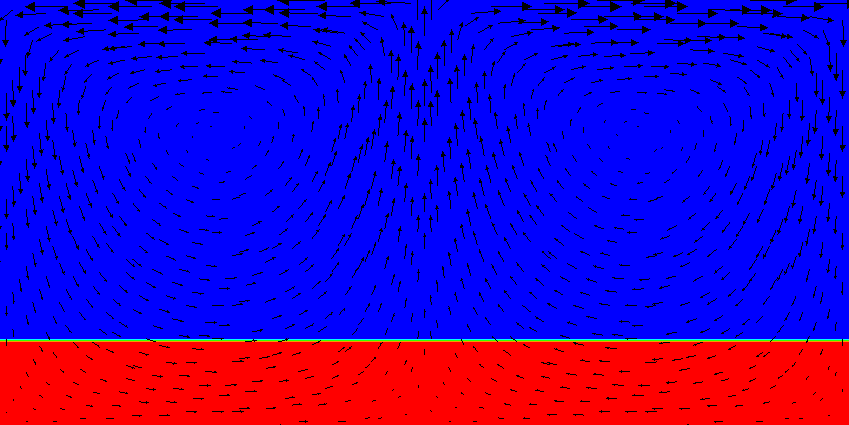
\includegraphics[width=0.3\textwidth]{cookbooks/composition-active/visit0007.png}
  \hfill
  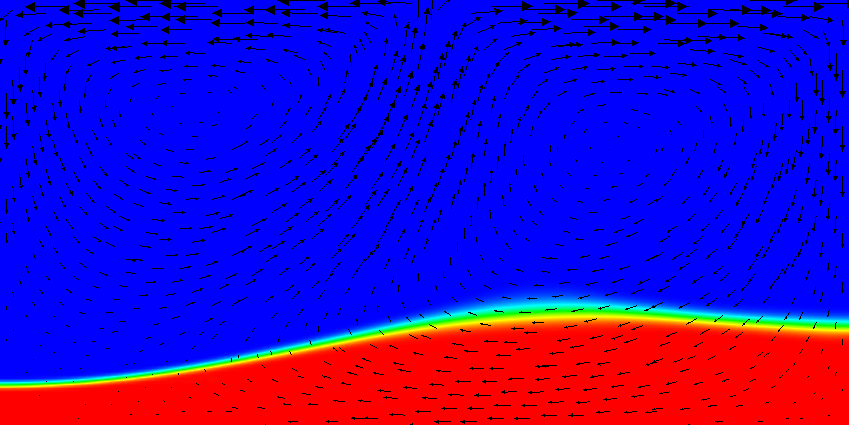
\includegraphics[width=0.3\textwidth]{cookbooks/composition-active/visit0009.png}
  \hfill
  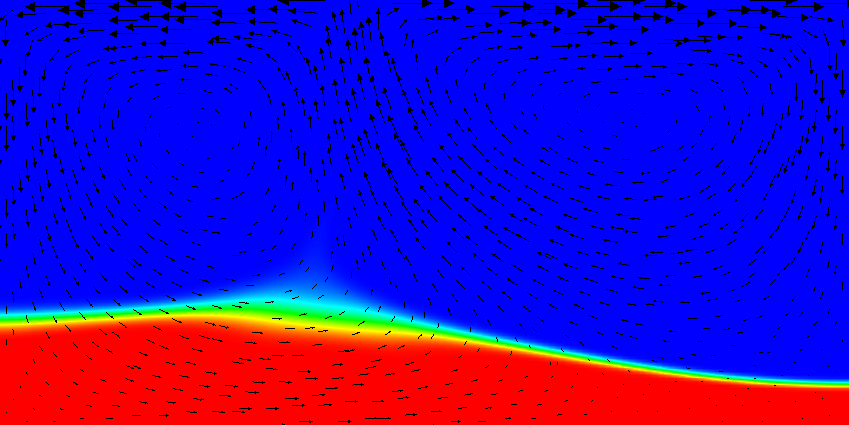
\includegraphics[width=0.3\textwidth]{cookbooks/composition-active/visit0008.png}
  \caption{Active compositional fields: Compositional field 1 at the time
    $t=0, 10, 20$. Compared to the results shown in
    Fig.~\ref{fig:compositional-passive} it is clear that the heavy material
    stays at the bottom of the domain now. The effect of the density on the
    velocity field is also clearly visible by noting that at all three times
    the spreading center at the top boundary is in exactly the same position;
    this would result in exactly the same velocity field if the density and
    temperature were constant.}
  \label{fig:composition-active-composition}
\end{figure}

\begin{figure}
  \centering
  \centering
  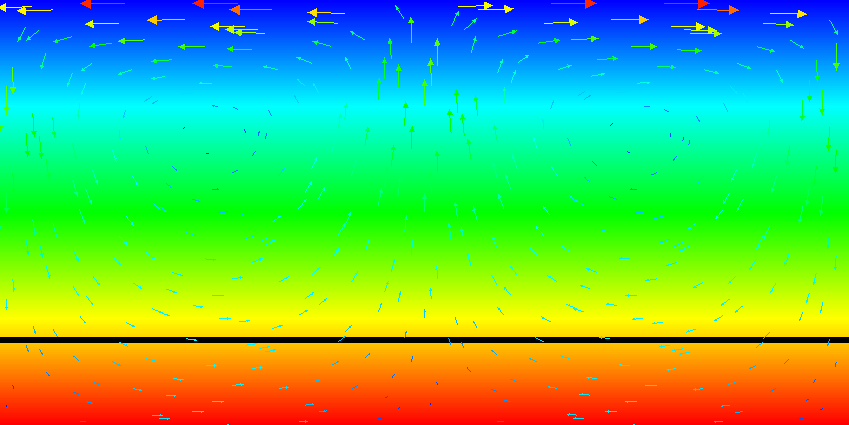
\includegraphics[width=0.3\textwidth]{cookbooks/composition-active/visit0000.png}
  \hfill
  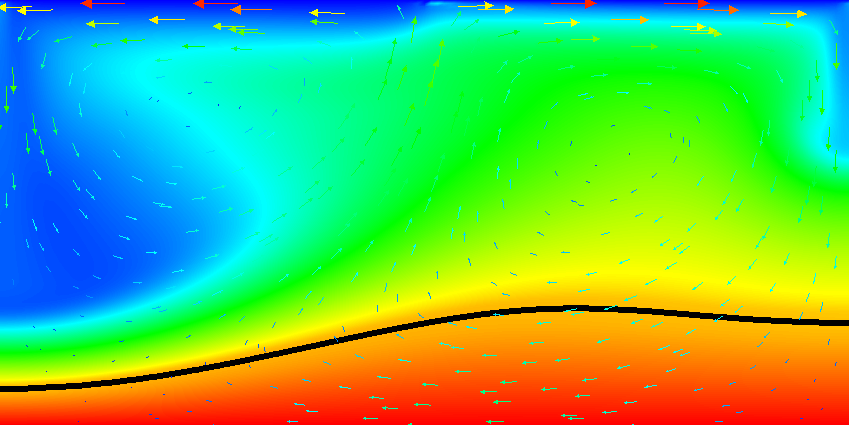
\includegraphics[width=0.3\textwidth]{cookbooks/composition-active/visit0001.png}
  \hfill
  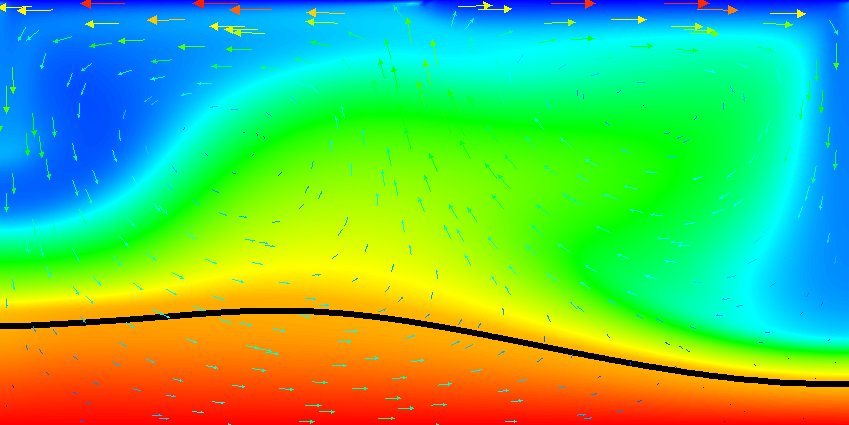
\includegraphics[width=0.3\textwidth]{cookbooks/composition-active/visit0002.png}
  \\
  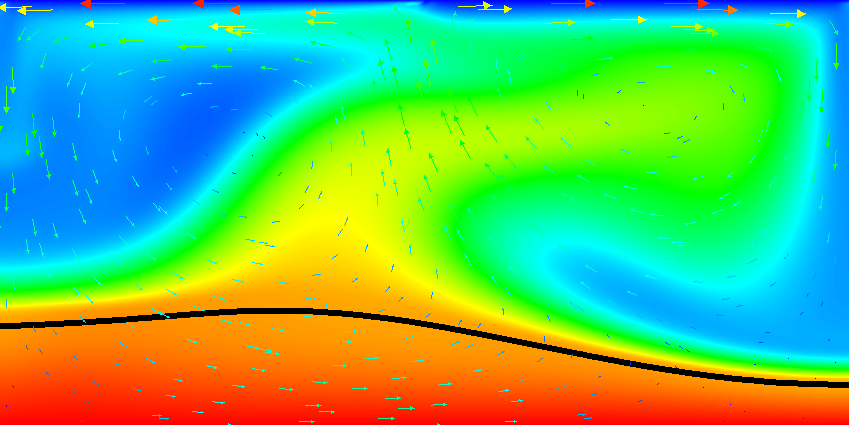
\includegraphics[width=0.3\textwidth]{cookbooks/composition-active/visit0003.png}
  \hfill
  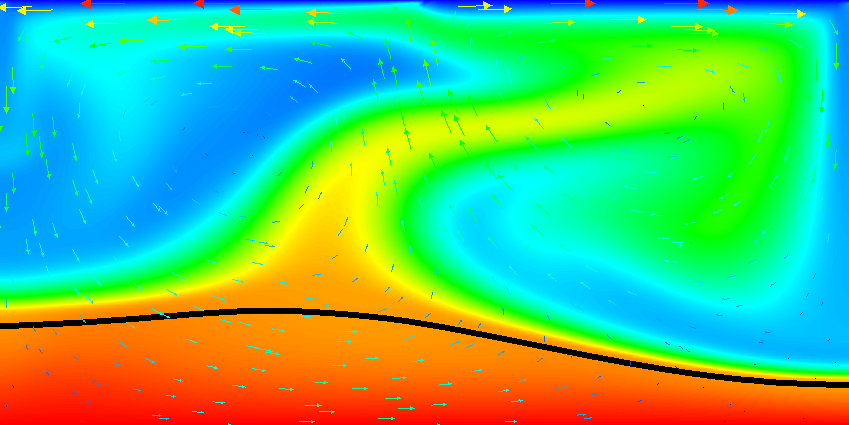
\includegraphics[width=0.3\textwidth]{cookbooks/composition-active/visit0004.png}
  \hfill
  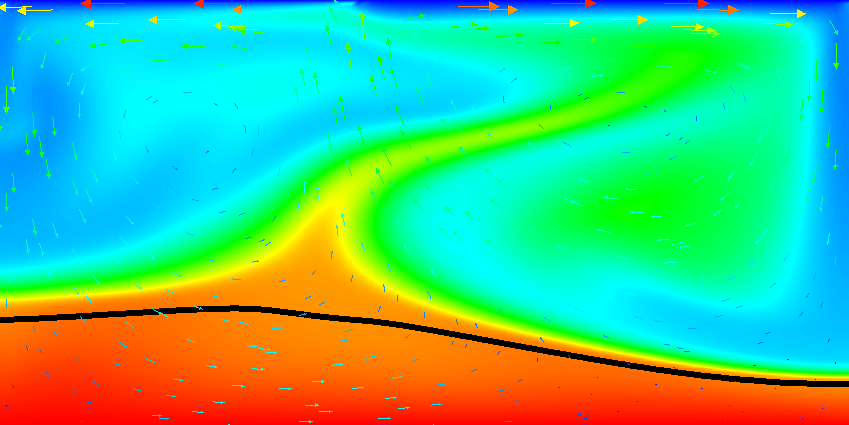
\includegraphics[width=0.3\textwidth]{cookbooks/composition-active/visit0006.png}
  \caption{Active compositional fields: Temperature fields at $t=0, 2, 4, 8, 12,
    20$. The black line is the isocontour line $c_1(\vec x,t)=0.5$
    delineating the position of the dense material at the bottom.}
  \label{fig:composition-active-temperature}
\end{figure}

Results of this model are visualized in
Fig.s~\ref{fig:composition-active-composition} and \ref{fig:composition-active-temperature}. What is visible is
that over the course of the simulation, the material that starts at the bottom
of the domain remains there. This can only happen if the circulation is
significantly affected by the high density material once the interface starts
to become non-horizontal, and this is
indeed visible in the velocity vectors. As a second consequence, if the
material at the bottom does not move away, then there needs to be a different
way for the heat provided at the bottom to get through the bottom layer:
either there must be a secondary convection system in the bottom layer, or
heat is simply conducted. The pictures in the figure seem to suggest
that the latter is the case.

It is easy, using the
outline above, to play with the various factors that drive this system, namely:
\begin{itemize}
  \item The magnitude of the velocity prescribed at the top.
  \item The magnitude of the velocities induced by thermal buoyancy, as
  resulting from the magnitude of gravity and the thermal expansion coefficient.
  \item The magnitude of the velocities induced by compositional variability, as
  described by the coefficient $\gamma$ and the magnitude of gravity.
\end{itemize}
Using the coefficients involved in these considerations, it is trivially
possible to map out the parameter space to find which of these effects is
dominant. As mentioned in discussing the values in the input file, what is
important is the \textit{relative} size of these parameters, not the fact
that currently the density in the material at the bottom is 100 times larger
than in the rest of the domain, an effect that from a physical perspective
clearly makes no sense at all.



\subsubsection{Using tracer particles}
\marginpar{To be written}


\subsection{Geophysical setups}
\label{sec:cookbooks-geophysical}
\marginpar{To be written}

Include something that uses the GPlates interface

\subsection{Benchmarks}
\label{sec:cookbooks-benchmarks}

Benchmarks are used to verify that a solver solves the problem correctly,
i.e., to \textit{verify} correctness of a code.%
\footnote{Verification is the first half of the \textit{verification and
    validation} (V\&V) procedure: \textit{verification} intends to ensure that the
  mathematical model is solved correctly, while \textit{validation} intends to
  ensure that the mathematical model is correct. Obviously, much of the aim of
  computational geodynamics is to validate the models that we have.}
Over the past decades, the geodynamics community has come up with a large
number of benchmarks. Depending on the goals of their original inventors, they
describe stationary problems in which only the solution of the flow problem is
of interest (but the flow may be compressible or incompressible, with constant
or variable viscosity, etc), or they may actually model time-dependent
processes. Some of them have solutions that are analytically known and can be
compared with, while for others, there are only sets of numbers that are
approximately known. We have implemented a number of them in \aspect{} to
convince ourselves (and our users) that \aspect{} indeed works as intended and
advertised. Some of these benchmarks are discussed below. Numerical results
for these benchmarks are also presented in \cite{KHB12} in much more detail
than shown here.


\subsubsection{The SolCx Stokes benchmark}
\label{sec:benchmark-solcx}

The SolCx benchmark is intended to test the accuracy of the solution to a
problem that has a large jump in the viscosity along a line through the
domain. Such situations are common in geophysics: for example, the viscosity
in a cold, subducting slab is much larger than in the surrounding, relatively
hot mantle material.

The SolCx benchmark computes the Stokes flow field of a fluid driven by
spatial density variations, subject to a spatially variable
viscosity. Specifically, the domain is $\Omega=[0,1]^2$, gravity is $\mathbf
g=(0,-1)^T$ and the density is given
by $\rho(\mathbf x)=\sin(\pi x_1)\cos(\pi x_2)$; this can be considered a
density perturbation to a constant background density. The viscosity is
\begin{align*}
  \eta(\mathbf x) = \left\{
    \begin{matrix}
      1 & \text{for}\ x_1 \le 0.5, \\
      10^6 & \text{for}\ x_1  > 0.5.
    \end{matrix}
  \right.
\end{align*}
This strongly discontinuous viscosity field yields an almost stagnant flow in
the right half of the domain and consequently a singularity in the pressure
along the interface.
Boundary conditions are free slip on all of $\partial\Omega$. The temperature
plays no role in this benchmark. The prescribed density field and the
resulting velocity field are shown in Fig.~\ref{fig:solcx}.

The SolCx benchmark was previously used in \cite[Section 4.1.1]{DMGT11}
(references to earlier uses of the benchmark are available there) and its analytic
solution is given in \cite{Zho96}. \aspect{} contains an implementation of
this analytic solution taken from the Underworld package (see \cite{MQLMAM07}
and \url{http://www.underworldproject.org/}, and correcting for the mismatch
in sign between the implementation and the description in \cite{DMGT11}).

\begin{figure}
  \begin{center}
    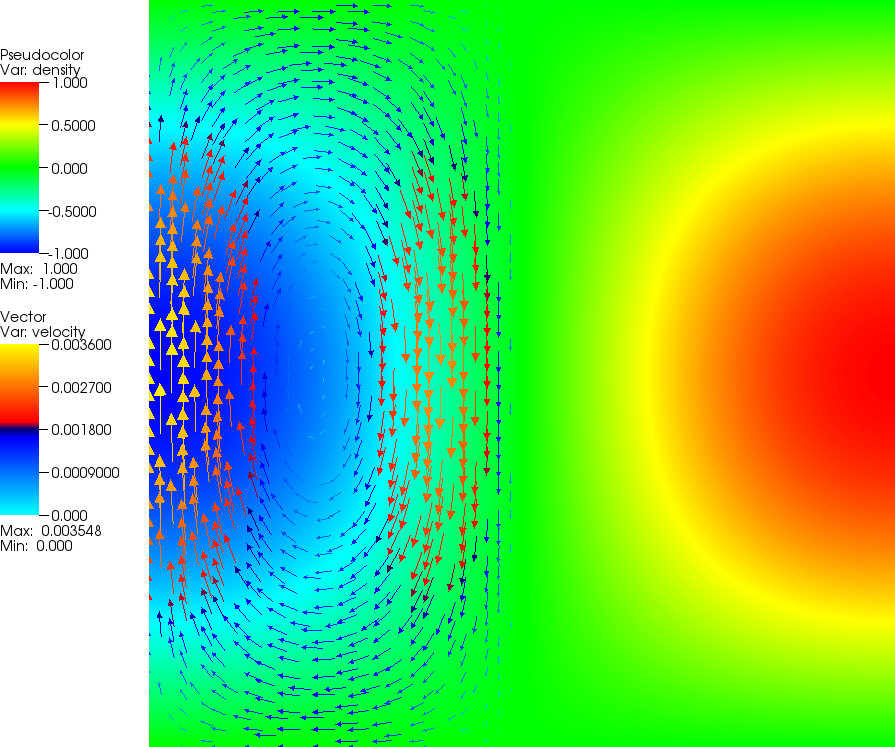
\includegraphics[width=0.45\textwidth]{cookbooks/benchmarks/solcx-solution}
    \hfill
    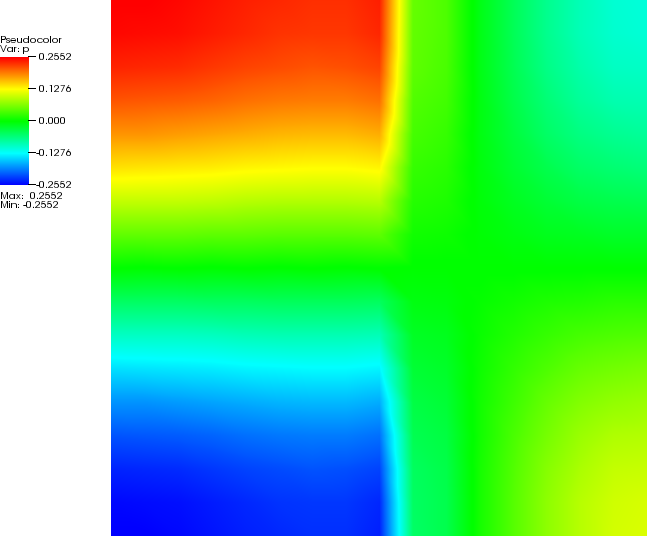
\includegraphics[width=0.45\textwidth]{cookbooks/benchmarks/solcx-solution-pressure}
    \caption{SolCx Stokes benchmark. Left: The density perturbation field and
      overlaid to it some velocity vectors. The viscosity is very large in the
      right hand, leading to a stagnant flow in this region. Right: The
      pressure on a relatively coarse mesh, showing the internal layer along
      the line where the viscosity jumps.}
    \label{fig:solcx}
  \end{center}
\end{figure}

To run this benchmark, the following input file will do:
\begin{lstlisting}[frame=single,language=prmfile]
############### Global parameters

set Dimension                              = 2

set Start time                             = 0
set End time                               = 0

set Output directory                       = output

set Pressure normalization                 = volume


############### Parameters describing the model

subsection Geometry model
  set Model name = box

  subsection Box
    set X extent = 1
    set Y extent = 1
  end
end


subsection Model settings
  set Prescribed velocity boundary indicators =
  set Tangential velocity boundary indicators = 0,1,2,3
  set Zero velocity boundary indicators       =
end


subsection Material model
  set Model name = SolCx

  subsection SolCx
    set Viscosity jump = 1e6
  end
end


subsection Gravity model
  set Model name = vertical
end


############### Parameters describing the temperature field

subsection Boundary temperature model
  set Model name = box
end


subsection Initial conditions
  set Model name = perturbed box
end



############### Parameters describing the discretization

subsection Discretization
  set Stokes velocity polynomial degree       = 2
  set Use locally conservative discretization = false
end


subsection Mesh refinement
  set Initial adaptive refinement              = 0
  set Initial global refinement                = 4
end


############### Parameters describing the what to do with the solution

subsection Postprocess
  set List of postprocessors = DuretzEtAl error, visualization
end
\end{lstlisting}

Since this is the first cookbook in the benchmarking section, let us go
through the different parts of this file in more detail:
\begin{itemize}
\item The first part consists of parameter setting for overall
  parameters. Specifically, we set the dimension in which this benchmark runs
  to two and choose an output directory. Since we are not interested in a time
  dependent solution, we set the end time equal to the start time, which
  results in only a single time step being computed.

  The last parameter of this section, \texttt{Pressure normalization},
\index[prmindex]{Pressure normalization}
\index[prmindexfull]{Pressure normalization}
  is set in such a way that the pressure is chosen so that its \textit{domain}
  average is zero, rather than the pressure along the surface, see
  Section~\ref{sec:pressure}.

\item The next part of the input file describes the setup of the
  benchmark. Specifically, we have to say how the geometry should look like (a
  box of size $1\times 1$) and what the velocity boundary conditions shall be
  (tangential flow all around -- the box geometry defines four boundary
\index[prmindex]{Model name}
\index[prmindexfull]{Geometry model!Model name}
  indicators for the left, right, bottom and top boundaries, see also
  Section~\ref{parameters:Geometry_20model}). This is followed by subsections
  choosing the material model (where we choose a particular model implemented
  in \aspect{} that describes the spatially variable density and viscosity
  fields, along with the size of the viscosity jump) and finally the chosen
  gravity model (a gravity field that is the constant vector $(0,-1)^T$, see
\index[prmindex]{Model name}
\index[prmindexfull]{Gravity model!Model name}
  Section~\ref{parameters:Gravity_20model}).

\item The part that follows this describes the boundary and initial values for
  the temperature. While we are not interested in the evolution of the
  temperature field in this benchmark, we nevertheless need to set
  something. The values given here are the minimal set of inputs.

\item The second-to-last part sets discretization parameters. Specifically, it
  determines what kind of Stokes element to choose (see
\index[prmindex]{Stokes velocity polynomial degree}
\index[prmindexfull]{Discretization!Stokes velocity polynomial degree}
  Section~\ref{parameters:Discretization} and the extensive discussion in
  \cite{KHB12}). We do not adaptively refine the mesh but only do four global
  refinement steps at the very beginning. This is obviously a parameter worth
\index[prmindex]{Initial global refinement}
\index[prmindexfull]{Mesh refinement!Initial global refinement}
  playing with.

\item The final section on postprocessors determines what to do with the
  solution once computed. Here, we do two things: we ask \aspect{} to compute
  the error in the solution using the setup described in the Duretz et
  al.~paper \cite{DMGT11}, and we request that output files for later
  visualization are generated and placed in the output directory. The
  functions that compute the error automatically query which kind of material
  model had been chosen, i.e., they can know whether we are solving the SolCx
  benchmark or one of the other benchmarks discussed in the following
  subsections.
\end{itemize}

Upon running \aspect{} with this input file, you will get output of the
following kind (obviously with different timings, and details of the output
may also change as development of the code continues):
\begin{lstlisting}[frame=single,language=ksh]
aspect/cookbooks> ../lib/aspect sol_cx.prm
Number of active cells: 256 (on 5 levels)
Number of degrees of freedom: 3,556 (2,178+289+1,089)

*** Timestep 0:  t=0 years
   Solving temperature system... 0 iterations.
   Rebuilding Stokes preconditioner...
   Solving Stokes system... 30+3 iterations.

   Postprocessing:
     Errors u_L1, p_L1, u_L2, p_L2: 1.125997e-06, 2.994143e-03, 1.670009e-06, 9.778441e-03
     Writing graphical output:      output/solution-00000



+---------------------------------------------+------------+------------+
| Total wallclock time elapsed since start    |      1.51s |            |
|                                             |            |            |
| Section                         | no. calls |  wall time | % of total |
+---------------------------------+-----------+------------+------------+
| Assemble Stokes system          |         1 |     0.114s |       7.6% |
| Assemble temperature system     |         1 |     0.284s |        19% |
| Build Stokes preconditioner     |         1 |    0.0935s |       6.2% |
| Build temperature preconditioner|         1 |    0.0043s |      0.29% |
| Solve Stokes system             |         1 |    0.0717s |       4.8% |
| Solve temperature system        |         1 |  0.000753s |      0.05% |
| Postprocessing                  |         1 |     0.627s |        42% |
| Setup dof systems               |         1 |      0.19s |        13% |
+---------------------------------+-----------+------------+------------+
\end{lstlisting}

One can then visualize the solution in a number of different ways (see
Section~\ref{sec:viz}), yielding pictures like those shown in
Fig.~\ref{fig:solcx}. One can also analyze the error as shown in various
different ways, for example as a function of the mesh refinement level, the
element chosen, etc.; we have done so extensively in \cite{KHB12}.


\subsubsection{The SolKz Stokes benchmark}
\label{sec:benchmark-solkz}

The SolKz benchmark is another variation on the same theme as the SolCx
benchmark above: it solves a Stokes problem with a spatially variable
viscosity but this time the viscosity is not a discontinuous function but
grows exponentially with the vertical coordinate so that it's overall
variation is again $10^6$. The forcing is again chosen by imposing a spatially
variable density variation. For details, refer again to \cite{DMGT11}.

The following input file, only a small variation of the one in the previous
section, solves this benchmark:

\begin{lstlisting}[frame=single,language=prmfile]
############### Global parameters

set Dimension                              = 2

set Start time                             = 0
set End time                               = 0

set Output directory                       = output

set Pressure normalization                 = volume


############### Parameters describing the model

subsection Geometry model
  set Model name = box

  subsection Box
    set X extent = 1
    set Y extent = 1
  end
end


subsection Model settings
  set Prescribed velocity boundary indicators =
  set Tangential velocity boundary indicators = 0,1,2,3
  set Zero velocity boundary indicators       =
end


subsection Material model
  set Model name = SolKz
end


subsection Gravity model
  set Model name = vertical
end


############### Parameters describing the temperature field

subsection Boundary temperature model
  set Model name = box
end


subsection Initial conditions
  set Model name = perturbed box
end



############### Parameters describing the discretization

subsection Discretization
  set Stokes velocity polynomial degree       = 2
  set Use locally conservative discretization = false
end


subsection Mesh refinement
  set Initial adaptive refinement              = 0
  set Initial global refinement                = 4
end


############### Parameters describing the what to do with the solution

subsection Postprocess
  set List of postprocessors = DuretzEtAl error, visualization
end
\end{lstlisting}

The output when running \aspect{} on this parameter file looks similar to the
one shown for the SolCx case. The solution when computed with one more level
of global refinement is visualized in Fig.~\ref{fig:solkz}.

\begin{figure}
  \begin{center}
    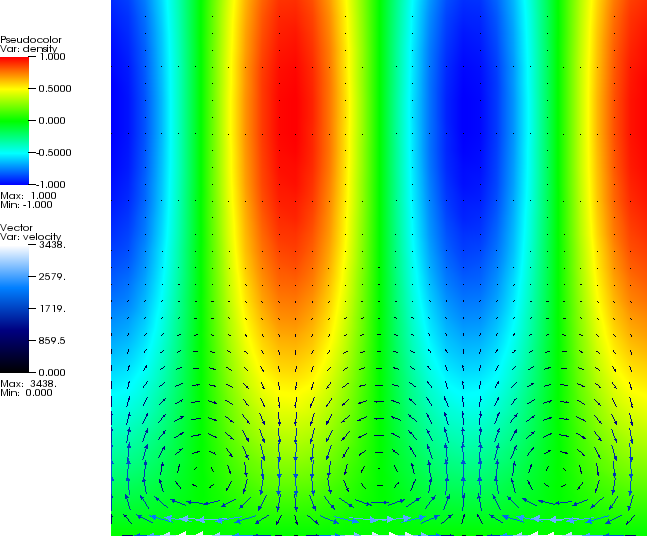
\includegraphics[width=0.45\textwidth]{cookbooks/benchmarks/solkz-solution}
    \hfill
    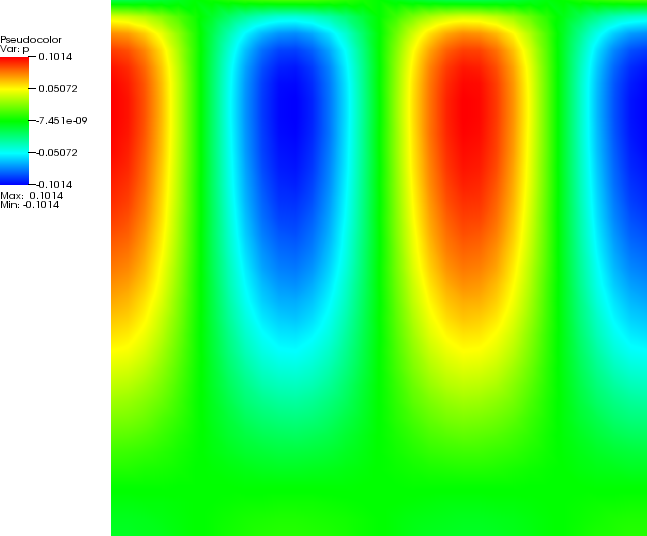
\includegraphics[width=0.45\textwidth]{cookbooks/benchmarks/solkz-solution-pressure}
    \caption{SolKz Stokes benchmark. Left: The density perturbation field and
      overlaid to it some velocity vectors. The viscosity grows exponentially
      in the vertical direction, leading to small velocities at the top
      despite the large density variations. Right: The
      pressure.}
    \label{fig:solkz}
  \end{center}
\end{figure}


\subsubsection{The ``inclusion'' Stokes benchmark}
\label{sec:benchmark-inclusion}

The ``inclusion'' benchmark again solves a problem with a discontinuous
viscosity, but this time the viscosity is chosen in such a way that the
discontinuity is along a circle. This ensures that, unlike in the SolCx
benchmark discussed above, the discontinuity in the viscosity never aligns to
cell boundaries, leading to much larger difficulties in obtaining an accurate
representation of the pressure. Specifically, the almost discontinuous
pressure along this interface leads to oscillations in the numerical
solution. This can be seen in the visualizations shown in
Fig.~\ref{fig:inclusion}. As before, for details we refer to
\cite{DMGT11}. The analytic solution against which we compare is given in
\cite{SP03}. An extensive discussion of convergence properties is given in
\cite{KHB12}.

\begin{figure}
  \begin{center}
    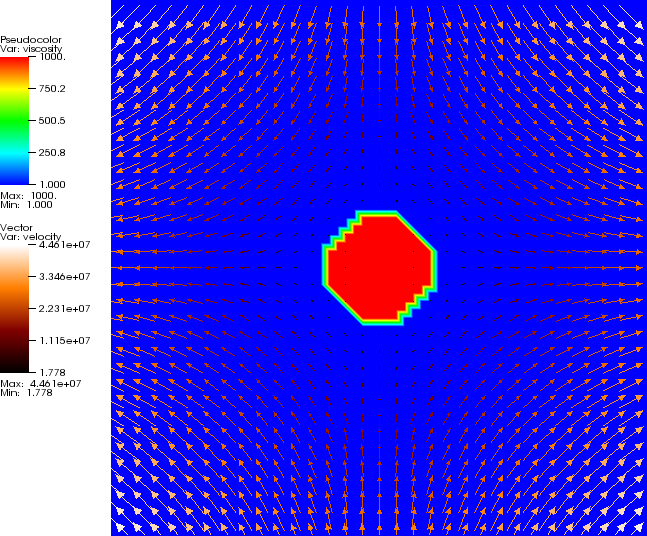
\includegraphics[width=0.45\textwidth]{cookbooks/benchmarks/inclusion-solution}
    \hfill
    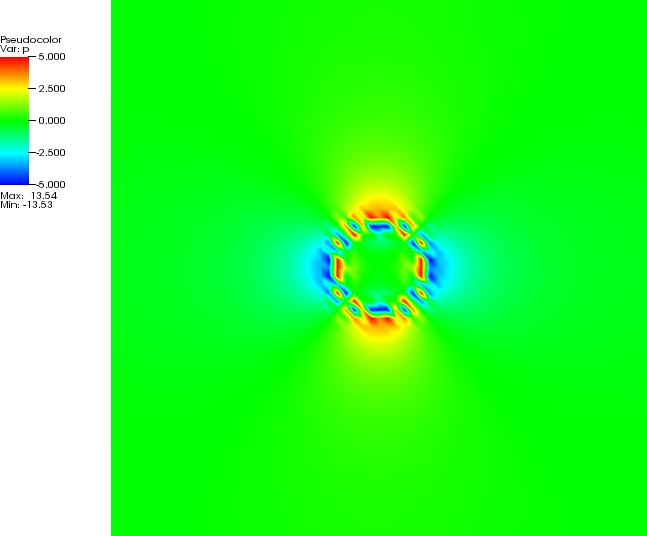
\includegraphics[width=0.45\textwidth]{cookbooks/benchmarks/inclusion-solution-pressure}
    \caption{Inclusion Stokes benchmark. Left: The viscosity field
      when interpolated onto the mesh (internally, the ``exact'' viscosity
      field -- large inside a circle, small outside -- is used),
      and overlaid to it some velocity vectors. Right: The
      pressure with its oscillations along the interface. The oscillations
      become more localized as the mesh is refined.}
    \label{fig:inclusion}
  \end{center}
\end{figure}

As before, the benchmark can be run with a small variation of the input files
already discussed above:
\marginpar{Revisit this once we have the machinery in place to choose nonzero
  boundary conditions in a more elegant way.}

\begin{lstlisting}[frame=single,language=prmfile]
############### Global parameters

set Dimension                              = 2

set Start time                             = 0
set End time                               = 0

set Output directory                       = output

set Pressure normalization                 = volume


############### Parameters describing the model

subsection Geometry model
  set Model name = box

  subsection Box
    set X extent = 2
    set Y extent = 2
  end
end


subsection Model settings
  set Prescribed velocity boundary indicators = 0,1,2,3
  set Tangential velocity boundary indicators =
  set Zero velocity boundary indicators       =
end


subsection Material model
  set Model name = Inclusion

  subsection Inclusion
    set Viscosity jump = 1e3
  end
end


subsection Gravity model
  set Model name = vertical
end


############### Parameters describing the temperature field

subsection Boundary temperature model
  set Model name = box
end


subsection Initial conditions
  set Model name = perturbed box
end



############### Parameters describing the discretization

subsection Discretization
  set Stokes velocity polynomial degree       = 2
  set Use locally conservative discretization = false
end


subsection Mesh refinement
  set Initial adaptive refinement              = 0
  set Initial global refinement                = 6
end


############### Parameters describing the what to do with the solution

subsection Postprocess
  set List of postprocessors = DuretzEtAl error, visualization
end
\end{lstlisting}

\subsubsection{The ``Stokes' law'' benchmark}
\label{sec:benchmark-stokes_law}

\textit{This section was contributed by Juliane Dannberg.}

Stokes' law was derived by George Gabriel Stokes in 1851 and describes the frictional force
a sphere with a density different than the surrounding fluid experiences in a
laminar flowing viscous medium.
A setup for testing this law is a sphere with the radius $r$ falling in a highly
viscous fluid with lower density. Due to its higher density the sphere is
accelerated by the gravitational force. While
the frictional force increases with the velocity of the falling particle,
the buoyancy force remains constant. Thus, after some time the forces will
be balanced and the settling velocity of the sphere $v_s$ will remain constant:

\begin{align}
  \label{eq:stokes-law}
  \underbrace{6 \pi \, \eta \, r \, v_s}_{\text{frictional force}} =
  \underbrace{4/3 \pi \, r^3 \, \Delta\rho \, g,}_{\text{buoyancy force}}
\end{align}
where $\eta$ is the dynamic viscosity of the fluid, $\Delta\rho$ is the
density difference between sphere and fluid and $g$ the gravitational
acceleration. The resulting settling velocity is then given by
\begin{align}
  \label{eq:stokes-velo}
  v_s = \frac{2}{9} \frac{\Delta\rho \, r^2 \, g}{\eta}.
\end{align}
Because we do not take into account inertia in our numerical computation,
the falling particle will reach the constant settling velocity right after
the first timestep.

For the setup of this benchmark, we chose the following parameters:
\begin{align*}
  \label{eq:stokes-parameters}
  r &= 200 \, \text{km}\\
  \Delta\rho &= 100 \, \text{kg}/\text{m}^3\\
  \eta &= 10^{22} \, \text{Pa s}\\
  g &= 9.81 \, \text{m}/\text{s}^2.
\end{align*}
With these values, the exact value of sinking velocity is $v_s =
8.72 \cdot 10^{-10} \, \text{m}/\text{s}$.

To run this benchmark, we need to set up an input file that describes the
situation. In principle, what we need to do is to describe a spherical object
with a density that is larger than the surrounding material. There are multiple
ways of doing this. For example, we could simply set the initial temperature of
the material in the sphere to a lower value, yielding a higher density with any
of the common material models. Or, we could use \aspect{}'s facilities to advect
along what are called ``compositional fields'' and make the density dependent on
these fields.

We will go with the second approach and tell \aspect{} to advect a single
compositional field. The initial conditions for this field will be zero outside
the sphere and one inside. We then need to also tell the material model to
increase the density by $\Delta\rho=100 kg\, m^{-3}$ times the concentration of
the compositional field. This can be done, like everything else, from the input
file.

All of this setup is then described by the following input file.
(You can find the input file to run this cookbook example in
\url{cookbooks/stokes.prm}. For your first runs you will probably want to
reduce the number of mesh refinement steps to make things run more quickly.)

\begin{lstlisting}[frame=single,language=prmfile,escapechar=\%]
############### Global parameters
# We use a 3d setup. Since we are only interested
# in a steady state solution, we set the end time
# equal to the start time to force a single time
# step before the program terminates.

set Dimension                              = 3 % \index[prmindex]{Dimension} \index[prmindexfull]{Dimension} %

set Start time                             = 0 % \index[prmindex]{Start time} \index[prmindexfull]{Start time} %
set End time                               = 0 % \index[prmindex]{End time} \index[prmindexfull]{End time} %
set Use years in output instead of seconds = false % \index[prmindex]{Use years in output instead of seconds} \index[prmindexfull]{Use years in output instead of seconds} %

set Output directory                       = output % \index[prmindex]{Output directory} \index[prmindexfull]{Output directory} %


############### Parameters describing the model
# The setup is a 3d box with edge length 2890000 in which
# all 6 sides have free slip boundary conditions. Because
# the temperature plays no role in this model we need not
# bother to describe temperature boundary conditions or
# the material parameters that pertain to the temperature.


subsection Geometry model
  set Model name = box % \index[prmindex]{Model name} \index[prmindexfull]{Geometry model!Model name} %

  subsection Box
    set X extent  = 2890000 % \index[prmindex]{X extent} \index[prmindexfull]{Geometry model!Box!X extent} %
    set Y extent  = 2890000 % \index[prmindex]{Y extent} \index[prmindexfull]{Geometry model!Box!Y extent} %
    set Z extent  = 2890000 % \index[prmindex]{Z extent} \index[prmindexfull]{Geometry model!Box!Z extent} %
  end
end


subsection Model settings
  set Tangential velocity boundary indicators = 0,1,2,3,4,5 % \index[prmindex]{Tangential velocity boundary indicators} \index[prmindexfull]{Model settings!Tangential velocity boundary indicators} %
end


subsection Material model
  set Model name = simple % \index[prmindex]{Model name} \index[prmindexfull]{Material model!Model name} %

  subsection Simple model
    set Reference density             = 3300 % \index[prmindex]{Reference density} \index[prmindexfull]{Material model!Simple model!Reference density} %
    set Viscosity                     = 1e22 % \index[prmindex]{Viscosity} \index[prmindexfull]{Material model!Simple model!Viscosity} %
  end
end


subsection Gravity model
  set Model name = vertical % \index[prmindex]{Model name} \index[prmindexfull]{Gravity model!Model name} %

  subsection Vertical
    set Magnitude = 9.81 % \index[prmindex]{Magnitude} \index[prmindexfull]{Gravity model!Vertical!Magnitude} %
  end
end


############### Parameters describing the temperature field
# As above, there is no need to set anything for the
# temperature boundary conditions.

subsection Boundary temperature model
  set Model name = box % \index[prmindex]{Model name} \index[prmindexfull]{Boundary temperature model!Model name} %
end

subsection Initial conditions
  set Model name = function % \index[prmindex]{Model name} \index[prmindexfull]{Initial conditions!Model name} %

  subsection Function
    set Function expression = 0 % \index[prmindex]{Function expression} \index[prmindexfull]{Initial conditions!Function!Function expression} %
  end
end

############### Parameters describing the compositional field
# This, however, is the more important part: We need to describe
# the compositional field and its influence on the density
# function. The following blocks say that we want to
# advect a single compositional field and that we give it an
# initial value that is zero outside a sphere of radius
# r=200000m and centered at the point (p,p,p) with
# p=1445000 (which is half the diameter of the box) and one inside.
# The last block re-opens the material model and sets the
# density differential per unit change in compositional field to
# 100.

subsection Compositional fields
  set Number of fields = 1 % \index[prmindex]{Number of fields} \index[prmindexfull]{Compositional fields!Number of fields} %
end

subsection Compositional initial conditions
  set Model name = function % \index[prmindex]{Model name} \index[prmindexfull]{Compositional initial conditions!Model name} %

  subsection Function
    set Variable names      = x,y,z % \index[prmindex]{Variable names} \index[prmindexfull]{Compositional initial conditions!Function!Variable names} %
    set Function constants  = r=200000,p=1445000 % \index[prmindex]{Function constants} \index[prmindexfull]{Compositional initial conditions!Function!Function constants} %
    set Function expression = if(sqrt((x-p)*(x-p)+(y-p)*(y-p)+(z-p)*(z-p)) > r, 0, 1) % \index[prmindex]{Function expression} \index[prmindexfull]{Compositional initial conditions!Function!Function expression} %
  end
end

subsection Material model
  subsection Simple model
    set Density differential for compositional field 1 = 100 % \index[prmindex]{Density differential for compositional field 1} \index[prmindexfull]{Material model!Simple model!Density differential for compositional field 1} %
  end
end




############### Parameters describing the discretization
# The following parameters describe how often we want to refine
# the mesh globally and adaptively, what fraction of cells should
# be refined in each adaptive refinement step, and what refinement
# indicator to use when refining the mesh adaptively.

subsection Mesh refinement
  set Initial adaptive refinement        = 4 % \index[prmindex]{Initial adaptive refinement} \index[prmindexfull]{Mesh refinement!Initial adaptive refinement} %
  set Initial global refinement          = 4 % \index[prmindex]{Initial global refinement} \index[prmindexfull]{Mesh refinement!Initial global refinement} %
  set Refinement fraction                = 0.2 % \index[prmindex]{Refinement fraction} \index[prmindexfull]{Mesh refinement!Refinement fraction} %
  set Strategy                           = velocity % \index[prmindex]{Strategy} \index[prmindexfull]{Mesh refinement!Strategy} %
end


############### Parameters describing the what to do with the solution
# The final section allows us to choose which postprocessors to
# run at the end of each time step. We select to generate graphical
# output that will consist of the primary variables (velocity, pressure,
# temperature and the compositional fields) as well as the density and
# viscosity. We also select to compute some statistics about the
# velocity field.

subsection Postprocess
  set List of postprocessors = visualization, velocity statistics % \index[prmindex]{List of postprocessors} \index[prmindexfull]{Postprocess!List of postprocessors} %

  subsection Visualization
    set List of output variables = density, viscosity % \index[prmindex]{List of output variables} \index[prmindexfull]{Postprocess!Visualization!List of output variables} %
  end
end
\end{lstlisting}

Usig this input file, let us try to evaluate the results of the current
computations for the settling velocity of the sphere. You can visualize the output in different
ways, one of it being ParaView and shown in
Fig.~\ref{fig:stokes-falling-sphere-2d} (an alternative is to use Visit as
described in Section~\ref{sec:viz}; 3d images of this simulation using Visit
are shown in Fig.~\ref{fig:stokes-falling-sphere-3d}).
Here, Paraview has the advantage that you can calculate the average velocity
of the sphere using the following filters:
\begin{enumerate}
 \item Threshold (Scalars: C\_1, Lower Threshold 0.5, Upper Threshold 1),
 \item Integrate Variables,
 \item Cell Data to Point Data,
 \item Calculator (use the formula sqrt(velocity\_x\textasciicircum2+
       velocity\_y\textasciicircum2+velocity\_z\textasciicircum2)/Volume).
\end{enumerate}
If you then look at
the Calculator object in the Spreadsheet View, you can see the average sinking
velocity of the sphere in the column ``Result'' and compare it to the theoretical
value $v_s = 8.72 \cdot 10^{-10} \, \text{m}/\text{s}$.
In this case, the numerical result is 8.865 $\cdot 10^{-10} \,
\text{m}/\text{s}$ when you add a few more refinement steps to actually resolve
the 3d flow field adequately. The ``velocity statistics'' postprocessor we have
selected above also provides us with a maximal velocity that is on the same
order of magnitude. The difference between the analytical and the numerical
values can be explained by different at least the following three points:
(i) In our case the sphere is viscous and not rigid as assumed in Stokes' initial model, leading to
a velocity field that varies inside the sphere rather than being constant.
(ii) Stokes' law is derived using an infinite domain but we have a finite box
instead. (iii) The mesh may not yet fine enough to provide a fully converges
solution. Nevertheless, the fact that we get a result that is accurate to less
than 2\% is a good indication that \aspect{} implements the equations correctly.

\begin{figure}
  \begin{center}
    \includegraphics[width=0.55\textwidth]{cookbooks/benchmarks/stokes/stokes-velocity}
    \hfill
    \includegraphics[width=0.44\textwidth]{cookbooks/benchmarks/stokes/stokes-density}
  \end{center}
  \caption{Stokes benchmark. Both figures show only a 2D slice of the
      three-dimensional model.
      Left: The compositional field and overlaid to it some velocity vectors.
      The composition is 1 inside a sphere with the radius of 200 km and 0
      outside of this sphere. As the velocity vectors show, the sphere sinks
      in the viscous medium.
      Right: The density distribution of the model. The compositional density
      contrast of 100 kg$/\text{m}^3$ leads to a higher density inside of the
      sphere.}
  \label{fig:stokes-falling-sphere-2d}
\end{figure}

\begin{figure}
  \begin{center}
    \includegraphics[width=0.3\textwidth]{cookbooks/benchmarks/stokes/composition}
    \hfill
    \includegraphics[width=0.3\textwidth]{cookbooks/benchmarks/stokes/mesh}
    \hfill
    \includegraphics[width=0.3\textwidth]{cookbooks/benchmarks/stokes/velocity}
  \end{center}
  \caption{Stokes benchmark. Three-dimensional views of the compositional field
  (left), the adaptively refined mesh (center) and the resulting velocity field
  (right).}
  \label{fig:stokes-falling-sphere-3d}
\end{figure}




\section{Extending \aspect}
\label{sec:extending}

\aspect{} is designed to be an extensible code. In particular, the program
uses a plugin architecture in which it is trivial to replace
or extend certain components of the program:
\begin{itemize}
\item the material description,
\item the geometry,
\item the gravity description,
\item the initial conditions,
\item the boundary conditions,
\item the functions that postprocess the solution, i.e., that can compute
  derived quantities such as heat fluxes over part of the boundary, mean
  velocities, etc.,
\item the functions that generate derived quantities that can be put into
  graphical output files for visualization such as fields that depict the
  strength of the friction heating term, spatially dependent actual
  viscosities, and so on,
\item the computation of refinement indicators,
\item the determination of how long a computation should run.
\end{itemize}
We will discuss the way this is achieved in Sections~\ref{sec:plugins} and
\ref{sec:plugins-concrete}. Changing the core functionality, i.e., the basic equations
\eqref{eq:stokes-1}--\eqref{eq:temperature}, and how they are solved is
arguably more involved. We will discuss this in Section
\ref{sec:extending-solver}.

In either of these two cases, you will need to extend the source code of the
program. Since \aspect{} is written in C++ using the \dealii{} library, you
will have to be proficient in C++. You will also likely have
to familiarize yourself with this library for which there is an extensive
amount of documentation:
\begin{itemize}
\item The manual at
  \url{http://www.dealii.org/developer/doxygen/deal.II/index.html} that
  describes in detail what every class, function and variable in \dealii{}
  does.
\item A collection of modules at
  \url{http://www.dealii.org/developer/doxygen/deal.II/modules.html} that give
  an overview of whole groups of classes and functions and how they work
  together to achieve their goal.
\item The \dealii{} tutorial at
  \url{http://www.dealii.org/developer/doxygen/tutorial/index.html} that
  provides a step-by-step introduction to the library using a sequence of
  several dozen programs that introduce gradually more complex topics. In
  particular, you will learn \dealii's way of \textit{dimension independent
  programming} that allows you to write the program once, test it in 2d, and
  run the exact same code in 3d without having to debug it a second time.
\item The step-31 and step-32 tutorial programs at
  \url{http://www.dealii.org/developer/doxygen/deal.II/step_31.html} and
  \url{http://www.dealii.org/developer/doxygen/deal.II/step_32.html} from
  which \aspect{} directly descends.
\item The \dealii{} Frequently Asked Questions at
  \url{http://dealii.sourceforge.net/index.php/Deal.II_Questions_and_Answers}
  that also have extensive sections on developing code with \dealii{} as well
  as on debugging. It also answers a number of questions we frequently get
  about the use of C++ in \dealii{}.
\item Several other parts of the \dealii{} website at
  \url{http://www.dealii.org/} also have information that may be relevant if
  you dive deeper into developing code. If you have questions, the mailing
  lists at \url{http://www.dealii.org/mail.html} are also of general help.
\item A general overview of \dealii{} is also provided in the paper
  \cite{BHK07}.
\end{itemize}

As a general note, by default \aspect{} utilizes a \dealii{} feature called \textit{debug
  mode}, see also the introduction to this topic in
Section~\ref{sec:debug-mode}. If you develop code, you will definitely want
this feature to be on, as it will capture the vast majority of bugs you
will invariably introduce in your code.

When you write new functionality and run
the code for the first time, you will almost invariably first have to deal
with a number of these assertions that point out problems in your code. While
this may be annoying at first, remember that these are actual bugs in your
code that have to be fixed anyway and that are much easier to find if the
program aborts than if you have to go by their more indirect results such as
wrong answers. The Frequently Asked Questions at
\url{http://dealii.sourceforge.net/index.php/Deal.II_Questions_and_Answers}
contain a section on how to debug \dealii{} programs.

The downside of debug mode, as mentioned before, is that it makes the program
much slower. Consequently, once you are
confident that your program actually does what it is intended to do --
\textbf{but no earlier!} --, you may want to switch to optimized mode that
links \aspect{} with a version of the \dealii{} libraries that uses compiler
optimizations and that does not contain the \texttt{assert} statements
discussed above. This switch can be facilitated by editing the top of the
\aspect{} \url{Makefile} and recompiling the program.

In addition to these general comments, \aspect{} is itself extensively
documented. You can find documentation on all classes, functions and
namespaces starting from the \url{doc/doxygen/index.html} page.


\subsection{The idea of plugins and the \texttt{SimulatorAccess} and \texttt{Introspection} classes}
\label{sec:plugins}

The most common modification you will probably want to do to \aspect{} are to
switch to a different material model (i.e., have different values of
functional dependencies for the coefficients $\eta,\rho,C_p, \ldots$ discussed
in Section~\ref{sec:coefficients}); change the geometry; change the direction
and magnitude of the gravity vector $\mathbf g$; or change the initial and
boundary conditions.

To make this as simple as possible, all of these parts of the program (and some more) have
been separated into modules that can be replaced quickly and where it is
simple to add a new implementation and make it available to the rest of the
program and the input parameter file. The way this is achieved is through the
following two steps:
\begin{itemize}
\item The core of \aspect{} really only communicates with material models,
  geometry descriptions, etc., through a simple and very basic
  interface. These interfaces are declared in the
  \url{include/aspect/material_model/interface.h},
  \url{include/aspect/geometry_model/interface.h}, etc., header files. These
  classes are always called \texttt{Interface}, are located in namespaces that
  identify their purpose, and their documentation can be found from the
  general class overview in \url{doc/doxygen/classes.html}.

  To show an example of a rather minimal case, here is the declaration of the
\href{doc/doxygen/classaspect_1_1GravityModel_1_1Interface.html}{aspect::GravityModel::Interface} class (documentation comments have
  been removed):
  \begin{lstlisting}[frame=single,language=C++]
    class Interface
    {
      public:
        virtual ~Interface();

        virtual
        Tensor<1,dim>
        gravity_vector (const Point<dim> &position) const = 0;

        static void declare_parameters (ParameterHandler &prm);

        virtual void parse_parameters (ParameterHandler &prm);
    };
  \end{lstlisting}

  If you want to implement a new model for gravity, you just need to write a
  class that derives from this base class and implements the
  \texttt{gravity\_vector} function. If your model wants to read parameters
  from the input file, you also need to have functions called
  \texttt{declare\_parameters} and \texttt{parse\_parameters} in your class
  with the same signatures as the ones above. On the other hand, if the new
  model does not need any run-time parameters, you do not need to overload
  these functions.%
  \footnote{At first glance one may think that only the
    \texttt{parse\_parameters} function can be overloaded since
    \texttt{declare\_parameters} is not virtual. However, while the latter is
    called by the class that manages plugins through pointers to the interface
    class, the former function is called essentially at the time of
    registering a plugin, from code that knows the actual type and name of the
    class you are implementing. Thus, it can call the function -- if it exists
    in your class, or the default implementation in the base class if it doesn't
    -- even without it being declared as virtual.}

  Each of the categories above that allow plugins have several implementations
  of their respective interfaces that you can use to get an idea of how to
  implement a new model.

\item At the end of the file where you implement your new model, you need to
  have a call to the macro \texttt{ASPECT\_REGISTER\_GRAVITY\_MODEL} (or the
  equivalent for the other kinds of plugins). For
  example, let us say that you had implemented a gravity model that takes
  actual gravimetric readings from the GRACE satellites into account, and had
  put everything that is necessary into a class
  \texttt{aspect::GravityModel::GRACE}. Then you need a statement like this at
  the bottom of the file:
  \begin{lstlisting}[frame=single,language=C++]
    ASPECT_REGISTER_GRAVITY_MODEL
    (GRACE,
     "grace",
     "A gravity model derived from GRACE "
     "data. Run-time parameters are read from the parameter "
     "file in subsection 'Radial constant'.");
  \end{lstlisting}
  Here, the first argument to the macro is the name of the class. The second
  is the name by which this model can be selected in the parameter file. And
  the third one is a documentation string that describes the purpose of the
  class (see, for example, Section~\ref{parameters:Gravity_20model} for an
  example of how existing models describe themselves).

  This little piece of code ensures several things: (i) That the parameters
  this class declares are known when reading the parameter file. (ii) That you
  can select this model (by the name ``grace'') via the run-time parameter
  \texttt{Gravity model/Model name}. (iii) That \aspect{} can create an object
  of this kind when selected in the parameter file.

  Note that you need not announce the existence of this class in any other
  part of the code: Everything should just work automatically.%
  \footnote{The existing implementations of models of the gravity and other interfaces
  declare the class in a header file and define the member functions in a
  \texttt{.cc} file. This is done so that these classes show up in our
  doxygen-generated documentation, but it is not necessary: you can put your
  entire class declaration and implementation into a single file as long as
  you call the macro discussed above on it. This single file is all you need
  to touch to add a new model.}
  This has the advantage that things are neatly separated: You do not need to
  understand the core of \aspect{} to be able to add a new gravity model that
  can then be selected in an input file. In fact, this is true for
  all of the plugins we have: by and large, they just receive some data
  from the simulator and do something with it (e.g., postprocessors), or they
  just provide information (e.g., initial meshes, gravity models), but they
  writing either does not imply that you have even fundamental understanding
  of what the core of the program does.
\end{itemize}

The procedure for the other areas where plugins are supported works
essentially the same, with the obvious change in namespace for the interface
class and macro name.

In the following, we will discuss the requirements for individual plugins. Before
doing so, however, let us discuss ways in which plugins can query other
information, in particular about the current state of the simulation.
To this end, let us not consider those plugins that by and large just
provide information without any context of the simulation, such as gravity models,
prescribed boundary velocities, or initial temperatures. Rather, let us
consider things like postprocessors that can compute things like boundary heat
fluxes. Taking this as an example (see Section~\ref{sec:postprocessors}), you are
required to write a function with the following interface
\begin{lstlisting}[frame=single,language=C++]
    template <int dim>
    class MyPostprocessor : public aspect::Postprocess::Interface
    {
      public:
        virtual
        std::pair<std::string,std::string>
        execute (TableHandler &statistics);

      // ... more things ...
\end{lstlisting}
The idea is that in the implementation of the \texttt{execute} function
you would compute whatever you are interested in (e.g., heat fluxes)
and return this information in the statistics object that then gets written
to a file (see Sections~\ref{sec:running-overview} and \ref{sec:viz-stat}).
A postprocessor may also generate other files if it so likes -- e.g., graphical
output, a file that stores the locations of tracers, etc.
To do so, obviously you need access to the current solution. This is
stored in a vector somewhere in the core of \aspect{}. However, this
vector is, by itself, not sufficient: you also need to know the finite
element space it is associated with, and for that the triangulation it
is defined on. Furthermore, you may need to know what the current
simulation time is. A variety of other pieces of information enters
computations in these kinds of plugins.

All of this information is of course part of the core of \aspect{},
as part of the
\href{doc/doxygen/classaspect_1_1Simulator.html}{aspect::Simulator
class}. However, this is a rather heavy class: it's got dozens of
member variables and functions, and it is the one that does all
of the numerical heavy lifting. Furthermore, to access data in
this class would require that you need to learn about the internals,
the data structures, and the design of this class.
It would be poor design if plugins had to access information from this
core class directly. Rather, the way this works is that those plugin
classes that wish to access information about the state of the simulation
inherit from the
\href{doc/doxygen/classaspect_1_1SimulatorAccess.html}{aspect::SimulatorAccess
class}. This class has an interface that looks like this:
\begin{lstlisting}[frame=single,language=C++]
    template <int dim>
    class SimulatorAccess
    {
    protected:
      double       get_time () const;

      std::string  get_output_directory () const;

      const LinearAlgebra::BlockVector &
      get_solution () const;

      const DoFHandler<dim> &
      get_dof_handler () const;

      // ... many more things ...
\end{lstlisting}
This way, \href{doc/doxygen/classaspect_1_1SimulatorAccess.html}{SimulatorAccess} makes information available to plugins
without the need for them to understand details of the core of \aspect{}.
Rather, if the core changes, the \href{doc/doxygen/classaspect_1_1SimulatorAccess.html}{SimulatorAccess} class can still
provide exactly the same interface. Thus, it insulates plugins from having
to know the core. Equally importantly, since \href{doc/doxygen/classaspect_1_1SimulatorAccess.html}{SimulatorAccess} only
offers its information in a read-only way it insulates the core from
plugins since they can not interfere in the workings of the core except
through the interface they themselves provide to the core.

Using this class, if a plugin class \texttt{MyPostprocess} is then not only
derived from the corresponding \texttt{Interface} class but \textit{also}
from the \href{doc/doxygen/classaspect_1_1SimulatorAccess.html}{SimulatorAccess} class, then you can write a member
function of the following kind (a non-sensical but instructive example; see
Section~\ref{sec:postprocessors} for more details on what postprocessors do
and how they are implemented):%
\footnote{For complicated, technical reasons, in the code below we need to
	access elements of the \href{doc/doxygen/classaspect_1_1SimulatorAccess.html}{SimulatorAccess} class using the notation
	\texttt{this->get\_solution()}, etc. This is due to the fact that both the
	current class and the base class are templates. A long description of
	why it is necessary to use \texttt{this->} can be found in the \dealii{}
	Frequently Asked Questions.}
\begin{lstlisting}[frame=single,language=C++]
    template <int dim>
    std::pair<std::string,std::string>
    MyPostprocessor<dim>::execute (TableHandler &statistics)
    {
      // compute the mean value of vector component 'dim' of the solution
      // (which here is the pressure block) using a deal.II function:
      const double
        average_pressure = VectorTools::compute_mean_value (this->get_mapping(),
                                                            this->get_dof_handler(),
                                                            QGauss<dim>(2),
                                                            this->get_solution(),
                                                            dim);
      statistics.add_value ("Average pressure", average_pressure);

      // return that there is nothing to print to screen (a useful
      // plugin would produce something more elaborate here):
      return std::pair<std::string,std::string>();
    }
\end{lstlisting}

The second piece of information that plugins can use is called ``introspection''.
In the code snippet above, we had to use that the pressure variable is at
position \texttt{dim}. This kind of \textit{implicit knowledge} is usually
bad style: it is error prone because one can easily forget where each
component is located; and it is an obstacle to the extensibility of a code
if this kind of knowledge is scattered all across the code base.

Introspection is a way out of this dilemma. Using the \texttt{SimulatorAccess::introspection()}
function returns a reference to an object (of type
\href{doc/doxygen/structaspect_1_1Introspection.html}{aspect::Introspection})
that plugins can use to learn about these sort of conventions. For example,
\texttt{this->introspection().component\_mask.pressure} returns a
component mask (a deal.II concept that describes a list of booleans for each
component in a finite element that
are true if a component is part of a variable we would like to select and
false otherwise) that describes which component of the finite element
corresponds to the pressure. The variable, \texttt{dim}, we need above
to indicate that we want the pressure component can be accessed
as \texttt{this->introspection().component\_indices.pressure}. While this
is certainly not shorter than just writing \texttt{dim}, it may in
fact be easier to remember. It is most definitely less prone to
errors and makes it simpler to extend the code in the future because
we don't litter the sources with ``magic constants'' like the one
above.

This \href{doc/doxygen/structaspect_1_1Introspection.html}{aspect::Introspection} class
has a significant number of variables that can be used in this way, i.e.,
they provide symbolic names for things one frequently has to do and
that would otherwise require implicit knowledge of things such as the
order of variables, etc.


\subsection{Materials, geometries, gravitation and other plugin types}
\label{sec:plugins-concrete}

\subsubsection{Material models}
\label{sec:material-models}

\marginpar{Need to update this given the current state of the plugin}

\index[prmindex]{Model name}
\index[prmindexfull]{Material model!Model name}
The material model is responsible for describing the various coefficients in
the equations that \aspect{} solves. To implement a new material model, you
need to overload the \href{doc/doxygen/classaspect_1_1MaterialModel_1_1Interface.html}{aspect::MaterialModel::Interface} class and use
the \texttt{ASPECT\_REGISTER\_MATERIAL\_MODEL} macro to register your new
class. The implementation of the new class should be in namespace
\texttt{aspect::MaterialModel}.

Specifically, your new class needs to implement the basic interface:
\begin{lstlisting}[frame=single,language=C++]
    template <int dim>
    class aspect::MaterialModel::Interface
    {
      public:
        // Physical parameters used in the basic equations
        virtual double viscosity (const double                  temperature,
                                  const double                  pressure,
                                  const SymmetricTensor<2,dim> &strain_rate,
                                  const Point<dim>             &position) const = 0;

        virtual double density (const double      temperature,
                                const double      pressure,
                                const Point<dim> &position) const = 0;

        virtual double compressibility (const double temperature,
                                        const double pressure,
                                        const Point<dim> &position) const = 0;

        virtual double specific_heat (const double      temperature,
                                      const double      pressure,
                                      const Point<dim> &position) const = 0;

        virtual double thermal_expansion_coefficient (const double      temperature,
                                                      const double      pressure,
                                                      const Point<dim> &position) const;

        virtual double thermal_conductivity (const double temperature,
                                             const double pressure,
                                             const Point<dim> &position) const
                                             = 0;

        // Qualitative properties one can ask a material model
        virtual bool
        viscosity_depends_on (const NonlinearDependence::Dependence dependence) const = 0;

        virtual bool
        density_depends_on (const NonlinearDependence::Dependence dependence) const = 0;

        virtual bool
        compressibility_depends_on (const NonlinearDependence::Dependence dependence) const = 0;

        virtual bool
        specific_heat_depends_on (const NonlinearDependence::Dependence dependence) const = 0;

        virtual bool
        thermal_conductivity_depends_on (const NonlinearDependence::Dependence dependence) const = 0;

        virtual bool is_compressible () const = 0;

        // Partial derivatives of physical parameters
        virtual double
        viscosity_derivative (const double              temperature,
                              const double              pressure,
                              const Point<dim>         &position,
                              const NonlinearDependence::Dependence dependence) const;

        virtual double
        density_derivative (const double              temperature,
                            const double              pressure,
                            const Point<dim>         &position,
                            const NonlinearDependence::Dependence dependence) const;

        virtual double
        compressibility_derivative (const double              temperature,
                                    const double              pressure,
                                    const Point<dim>         &position,
                                    const NonlinearDependence::Dependence dependence) const;

        virtual double
        specific_heat_derivative (const double              temperature,
                                  const double              pressure,
                                  const Point<dim>         &position,
                                  const NonlinearDependence::Dependence dependence) const;

        virtual double
        thermal_conductivity_derivative (const double              temperature,
                                         const double              pressure,
                                         const Point<dim>         &position,
                                         const NonlinearDependence::Dependence dependence) const;

        // Reference quantities
        virtual double reference_viscosity () const = 0;

        virtual double reference_density () const = 0;

        virtual double reference_thermal_expansion_coefficient () const = 0;

        // Auxiliary material properties used for postprocessing
        virtual
        double
        seismic_Vp (const double      temperature,
                    const double      pressure) const;

        virtual
        double
        seismic_Vs (const double      temperature,
                    const double      pressure) const;
        virtual
        unsigned int
        thermodynamic_phase (const double      temperature,
                             const double      pressure) const;

        // Functions used in dealing with run-time parameters
        static
        void
        declare_parameters (ParameterHandler &prm);

        virtual
        void
        parse_parameters (ParameterHandler &prm);
    };
\end{lstlisting}
Here, the first set of functions refer to the coefficients $\eta,C_p,k,\rho$ in
equations \eqref{eq:stokes-1}--\eqref{eq:temperature}, each as a function of
temperature, pressure, position and, in the case of the viscosity, the strain
rate. Implementations of these methods may of course choose to ignore
dependencies on any of these arguments. The second set of functions describes
the nonlinear dependence of the various coefficients on pressure, temperature,
or strain rate, and the next block then provides the numerical values of these
dependencies. This information will be used in future versions of \aspect{} to
implement a fully nonlinear solution scheme based on, for example, a Newton
iteration. The remaining functions are used in postprocessing as well as
handling run-time parameters. The exact meaning of these member functions is
documented in the
\href{doc/doxygen/classaspect_1_1MaterialModel_1_1Interface.html}{aspect::MaterialModel::Interface
class documentation}. Note that some of the functions listed above have a
default implementation, as discussed on the documentation page just
mentioned.

The function \texttt{is\_compressible} returns whether we should consider the
material as compressible or not, see Section~\ref{sec:boussinesq} on the
Boussinesq model. As discussed there, incompressibility as described by this function
does not necessarily imply that the density is constant; rather, it
may still depend on temperature or pressure. In the current
context, compressibility simply means whether we should solve the contuity
equation as $\nabla \cdot (\rho \mathbf u)=0$ (compressible Stokes)
or as $\nabla \cdot \mathbf{u}=0$ (incompressible Stokes).

The purpose of the last two functions has been discussed in the general
overview of plugins above.



\subsubsection{Geometry models}
\label{sec:geometry-models}

\index[prmindex]{Model name}
\index[prmindexfull]{Geometry model!Model name}
The geometry model is responsible for describing the domain in which we want
to solve the equations. A domain is described in \dealii{} by a coarse mesh
and, if necessary, an object that characterizes the boundary. Together, these
two suffice to reconstruct any domain by adaptively refining the coarse mesh
and placing new nodes generated by refining cells onto the surface described
by the boundary object. The geometry model is also responsible to describe to
the rest of the code which parts of the boundary represent Dirichlet-type
(fixed temperature) or Neumann-type (no heat flux) boundaries for the
temperature, and where the velocity is considered zero or tangential to the
boundary. This information is encoded in functions that return which boundary
indicators represent these types of boundaries; in \dealii{}, a boundary
indicator is a number attached to each piece of the boundary that can be used
to represent the type of boundary a piece belongs to.

To implement a new geometry model, you
need to overload the
\href{doc/doxygen/classaspect_1_1GeometryModel_1_1Interface.html}{aspect::GeometryModel::Interface}
class and use
the \texttt{ASPECT\_REGISTER\_GEOMETRY\_MODEL} macro to register your new
class. The implementation of the new class should be in namespace
\texttt{aspect::GeometryModel}.

Specifically, your new class needs to implement the following basic interface:
\begin{lstlisting}[frame=single,language=C++]
    template <int dim>
    class aspect::GeometryModel::Interface
    {
      public:
        virtual
        void
        create_coarse_mesh (parallel::distributed::Triangulation<dim> &coarse_grid) const = 0;

        virtual
        double
        length_scale () const = 0;

        virtual
        double depth(const Point<dim> &position) const = 0;

        virtual
        Point<dim> representative_point(const double depth) const = 0;

        virtual
        double maximal_depth() const = 0;

        virtual
        std::set<types::boundary_id_t>
        get_used_boundary_indicators () const = 0;

        static
        void
        declare_parameters (ParameterHandler &prm);

        virtual
        void
        parse_parameters (ParameterHandler &prm);
    };
\end{lstlisting}
The kind of information these functions need to provide is extensively
discussed in the documentation of this interface class at
\href{doc/doxygen/classaspect_1_1GeometryModel_1_1Interface.html}{aspect::GeometryModel::Interface}.
The purpose of the last two functions has been discussed in the general
overview of plugins above.


The \texttt{create\_coarse\_mesh} function does not only create the actual
mesh (i.e., the locations of the vertices of the coarse mesh and how they
connect to cells) but it must also set the boundary indicators for all parts
of the boundary of the mesh. The \dealii{} glossary describes the purpose of
boundary indicators as follows:
\begin{quote}
  In a \texttt{Triangulation} object, every part of the boundary is associated with
  a unique number (of type \texttt{types::boundary\_id}) that is used to identify which
  boundary geometry object is responsible to generate new points when the mesh
  is refined. By convention, this boundary indicator is also often used to
  determine what kinds of boundary conditions are to be applied to a particular
  part of a boundary. The boundary is composed of the faces of the cells and, in 3d,
  the edges of these faces.

  By default, all boundary indicators of a mesh are zero, unless you are
  reading from a mesh file that specifically sets them to something different,
  or unless you use one of the mesh generation functions in namespace \texttt{GridGenerator}
  that have a 'colorize' option. A typical piece of code that sets the boundary
  indicator on part of the boundary to something else would look like
  this, here setting the boundary indicator to 42 for all faces located at
  $x=-1$:
  \begin{lstlisting}[frame=single,language=C++]
  for (typename Triangulation<dim>::active_cell_iterator
         cell = triangulation.begin_active();
       cell != triangulation.end();
       ++cell)
    for (unsigned int f=0; f<GeometryInfo<dim>::faces_per_cell; ++f)
      if (cell->face(f)->at_boundary())
        if (cell->face(f)->center()[0] == -1)
          cell->face(f)->set_boundary_indicator (42);
  \end{lstlisting}
  This calls functions \texttt{TriaAccessor::set\_boundary\_indicator}. In 3d, it may
  also be appropriate to call \texttt{TriaAccessor::set\_all\_boundary\_indicators} instead
  on each of the selected faces. To query the boundary indicator of a particular
  face or edge, use \texttt{TriaAccessor::boundary\_indicator}.

  The code above only sets the boundary indicators of a particular part
  of the boundary, but it does not by itself change the way the Triangulation
  class treats this boundary for the purposes of mesh refinement. For this,
  you need to call \texttt{Triangulation::set\_boundary} to associate a boundary
  object with a particular boundary indicator. This allows the Triangulation
  object to use a different method of finding new points on faces and edges
  to be refined; the default is to use a \texttt{StraightBoundary} object for all
  faces and edges. The results section of step-49 has a worked example that
  shows all of this in action.

  The second use of boundary indicators is to describe not only which geometry
  object to use on a particular boundary but to select a part of the boundary
  for particular boundary conditions. \textit{[...]}

  \textbf{Note:} Boundary indicators are inherited from mother faces and edges to
  their children upon mesh refinement. Some more information about boundary
  indicators is also presented in a section of the documentation of the
  Triangulation class.
\end{quote}

Two comments are in order here. First, if a coarse triangulation's faces
already accurately represent where you want to pose which boundary condition
(for example to set temperature values or determine which are no-flow and
which are tangential flow boundary conditions), then it is sufficient to set
these boundary indicators only once at the beginning of the program since they
will be inherited upon mesh refinement to the child faces. Here, \textit{at the
beginning of the program} is equivalent to inside the
\texttt{create\_coarse\_mesh())} function of the geometry module shown above
that generates the coarse mesh.

Secondly, however, if you can only accurately determine which boundary
indicator should hold where on a refined mesh -- for example because the
coarse mesh is the cube $[0,L]^3$ and you want to have a fixed velocity
boundary describing an extending slab only for those faces for which
$z>L-L_\text{slab}$ -- then you need a way to set the boundary indicator
for all boundary faces either to the value representing the slab or the fluid
underneath \textit{after every mesh refinement step}. By doing so, child faces
can obtain boundary indicators different from that of their parents. \dealii{}
triangulations support this kind of operations using a so-called
\textit{post-refinement signal}. In essence, what this means is that you can
provide a function that will be called by the triangulation immediately after
every mesh refinement step.

The way to do this is by writing a function that sets boundary
indicators and that will be called by the \texttt{Triangulation} class. The
triangulation does not provide a pointer to itself to the function being
called, nor any other information, so the trick is to get this information
into the function. C++ provides a nice mechanism for this that is best
explained using an example:
\begin{lstlisting}[frame=single,language=C++]
    #include <deal.II/base/std_cxx1x/bind.h>

    template <int dim>
    void set_boundary_indicators (parallel::distributed::Triangulation<dim> &triangulation)
    {
      ... set boundary indicators on the triangulation object ...
    }

    template <int dim>
    void
    MyGeometry<dim>::
    create_coarse_mesh (parallel::distributed::Triangulation<dim> &coarse_grid) const
    {
      ... create the coarse mesh ...

      coarse_grid.signals.post_refinement.connect
	(std_cxx1x::bind (&set_boundary_indicators<dim>,
			  std_cxx1x::ref(coarse_grid)));

    }
\end{lstlisting}

What the call to \texttt{std\_cxx1x::bind} does is to produce an object that
can be called like a function with no arguments. It does so by taking the
address of a function that does, in fact, take an argument but permanently fix
this one argument to a reference to the coarse grid triangulation. After each
refinement step, the triangulation will then call the object so created which
will in turn call \texttt{set\_boundary\_indicators<dim>} with the reference
to the coarse grid as argument.

This approach can be generalized. In the example above, we have used a global
function that will be called. However, sometimes it is necessary that this
function is in fact a member function of the class that generates the mesh,
for example because it needs to access run-time parameters. This can be
achieved as follows: assuming the \texttt{set\_boundary\_indicators()}
function has been declared as a (non-static, but possibly private) member
function of the \texttt{MyGeometry} class, then the following will work:
\begin{lstlisting}[frame=single,language=C++]
    #include <deal.II/base/std_cxx1x/bind.h>

    template <int dim>
    void
    MyGeometry<dim>::
    set_boundary_indicators (parallel::distributed::Triangulation<dim> &triangulation) const
    {
      ... set boundary indicators on the triangulation object ...
    }

    template <int dim>
    void
    MyGeometry<dim>::
    create_coarse_mesh (parallel::distributed::Triangulation<dim> &coarse_grid) const
    {
      ... create the coarse mesh ...

      coarse_grid.signals.post_refinement.connect
	(std_cxx1x::bind (&MyGeometry<dim>::set_boundary_indicators,
			  std_cxx1x::cref(*this),
			  std_cxx1x::ref(coarse_grid)));
    }
\end{lstlisting}
Here, like any other member function, \texttt{set\_boundary\_indicators}
implicitly takes a pointer or reference to the object it belongs to as first
argument. \texttt{std::bind} again creates an object that can be called like a
global function with no arguments, and this object in turn calls
\texttt{set\_boundary\_indicators} with a pointer to the current object and a
reference to the triangulation to work on. Note that because the
\texttt{create\_coarse\_mesh} function is declared as \texttt{const}, it is
necessary that the \texttt{set\_boundary\_indicators} function is also
declared \texttt{const}.

\note{For reasons that have to do with the way the
  \texttt{parallel::distributed::Triangulation} is implemented, functions that
  have been attached to the post-refinement signal of the triangulation are
  called more than once, sometimes several times, every time the triangulation
  is actually refined.}


\subsubsection{Gravity models}
\label{sec:gravity-models}

\index[prmindex]{Model name}
\index[prmindexfull]{Gravity model!Model name}
The gravity model is responsible for describing the magnitude and direction of
the gravity vector at each point inside the domain. To implement a new gravity model, you
need to overload the
\href{doc/doxygen/classaspect_1_1GravityModel_1_1Interface.html}{aspect::GravityModel::Interface}
class and use
the \texttt{ASPECT\_REGISTER\_GRAVITY\_MODEL} macro to register your new
class. The implementation of the new class should be in namespace
\texttt{aspect::GravityModel}.

Specifically, your new class needs to implement the following basic interface:
\begin{lstlisting}[frame=single,language=C++]
    template <int dim>
    class aspect::GravityModel::Interface
    {
      public:
        virtual
        Tensor<1,dim>
        gravity_vector (const Point<dim> &position) const = 0;

        virtual
        void
        update ();

        static
        void
        declare_parameters (ParameterHandler &prm);

        virtual
        void
        parse_parameters (ParameterHandler &prm);
    };
\end{lstlisting}
The kind of information these functions need to provide is discussed in the
documentation of this interface class at
\href{doc/doxygen/classaspect_1_1GravityModel_1_1Interface.html}{aspect::GravityModel::Interface}. The first needs to return a gravity
vector at a given position, whereas the second is called at the beginning of
each time step, for example to allow a model to update itself based on the
current time or the solution of the previous time step.
The purpose of the last two functions has been
discussed in the general overview of plugins above.


\subsubsection{Initial conditions}
\label{sec:initial-conditions}

\index[prmindex]{Model name}
\index[prmindexfull]{Initial conditions!Model name}
The initial conditions model is responsible for describing the initial
temperature distribution throughout the domain. It essentially has to provide
a function that for each point can return the initial temperature. Note that
the model \eqref{eq:stokes-1}--\eqref{eq:temperature} does not require initial
values for the pressure or velocity. However, if coefficients are nonlinear,
one can significantly reduce the number of initial nonlinear iterations if a
good guess for them is available; consequently, \aspect{} initializes the
pressure with the adiabatically computed hydrostatic pressure, and a zero
velocity. Neither of these two has to be provided by the objects considered in
this section.

To implement a new initial conditions model, you
need to overload the
\href{doc/doxygen/classaspect_1_1InitialConditions_1_1Interface.html}{aspect::InitialConditions::Interface}
class and use
the \texttt{ASPECT\_REGISTER\_INITIAL\_CONDITIONS} macro to register your new
class. The implementation of the new class should be in namespace
\texttt{aspect::InitialConditions}.

Specifically, your new class needs to implement the following basic interface:
\begin{lstlisting}[frame=single,language=C++]
    template <int dim>
    class aspect::InitialConditions::Interface
    {
      public:
        void
        initialize (const GeometryModel::Interface<dim>       &geometry_model,
                    const BoundaryTemperature::Interface<dim> &boundary_temperature,
                    const AdiabaticConditions<dim>            &adiabatic_conditions);

        virtual
        double
        initial_temperature (const Point<dim> &position) const = 0;

        static
        void
        declare_parameters (ParameterHandler &prm);

        virtual
        void
        parse_parameters (ParameterHandler &prm);
    };
\end{lstlisting}
The meaning of the first class should be clear. The purpose
of the last two functions has been discussed in the general overview of
plugins above.


\subsubsection{Prescribed velocity boundary conditions}
\label{sec:prescribed-velocity-boundary-conditions}

\index[prmindex]{Prescribed velocity boundary indicators}
\index[prmindexfull]{Model settings!Prescribed velocity boundary indicators}

\marginpar{To be written}

\subsubsection{Temperature boundary conditions}
\label{sec:temperature-boundary-conditions}

\index[prmindex]{Fixed temperature boundary indicators}
\index[prmindexfull]{Model settings!Fixed temperature boundary indicators}
The boundary conditions are responsible for describing the temperature values
at those parts of the boundary at which the temperature is fixed (see
Section~\ref{sec:geometry-models} for how it is determined which parts of the
boundary this applies to).

To implement a new boundary conditions model, you
need to overload the
\href{doc/doxygen/classaspect_1_1BoundaryTemperature_1_1Interface.html}{aspect::BoundaryTemperature::Interface}
class and use
the \texttt{ASPECT\_REGISTER\_BOUNDARY\_TEMPERATURE\_MODEL} macro to register your new
class. The implementation of the new class should be in namespace
\texttt{aspect::BoundaryTemperature}.

Specifically, your new class needs to implement the following basic interface:
\begin{lstlisting}[frame=single,language=C++]
    template <int dim>
    class aspect::BoundaryTemperature::Interface
    {
      public:
        virtual
        double
        temperature (const GeometryModel::Interface<dim> &geometry_model,
                     const unsigned int                   boundary_indicator,
                     const Point<dim>                    &location) const = 0;

        virtual
        double minimal_temperature () const = 0;

        virtual
        double maximal_temperature () const = 0;

        static
        void
        declare_parameters (ParameterHandler &prm);

        virtual
        void
        parse_parameters (ParameterHandler &prm);
    };
\end{lstlisting}
The first of these functions needs to provide the fixed temperature at the
given point. The geometry model and the boundary indicator of the particular
piece of boundary on which the point is located is also given as a hint in
determining where this point may be located; this may, for example, be used to
determine if a point is on the inner or outer boundary of a spherical
shell. The remaining functions are obvious, and are also
discussed in the documentation of this interface class at
\href{doc/doxygen/classaspect_1_1BoundaryTemperature_1_1Interface.html}{aspect::BoundaryTemperature::Interface}. The
purpose
of the last two functions has been discussed in the general overview of
plugins above.


\subsubsection{Postprocessors: Evaluating the solution after each time step}
\label{sec:postprocessors}

\index[prmindex]{List of postprocessors}
\index[prmindexfull]{Postprocess!List of postprocessors}
Postprocessors are arguably the most complex and powerful of the plugins
available in \aspect{} since they do not only passively provide any
information but can actually compute quantities derived from the
solution. They are executed once at the end of each time step and,
unlike all the other plugins discussed above, there can be an arbitrary number
of active postprocessors in the same program (for the plugins discussed in
previous sections it was clear that there is always exactly one material
model, geometry model, etc.).

\paragraph{Motivation.}
The original motivation for postprocessors is that the goal of a simulation is
of course not the simulation itself, but that we want to do something with the
solution. Examples for already existing postprocessors are:
\begin{itemize}
\item Generating output in file formats that are understood by visualization
  programs. This is facilitated by the
  \href{doc/doxygen/classaspect_1_1Postprocess_1_1Visualization.html}{aspect::Postprocess::Visualization}
  class and a separate class of visualization postprocessors, see
  Section~\ref{sec:viz-postpostprocessors}.
\item Computing statistics about the velocity field (e.g., computing minimal,
  maximal, and average velocities), temperature field (minimal, maximal, and
  average temperatures), or about the heat fluxes across boundaries of the
  domain. This is provided by the
  \href{doc/doxygen/classaspect_1_1Postprocess_1_1VelocityStatistics.html}{aspect::Postprocess::VelocityStatistics},
  \href{doc/doxygen/classaspect_1_1Postprocess_1_1TemperatureStatistics.html}{aspect::Postprocess::TemperatureStatistics},
  \href{doc/doxygen/classaspect_1_1Postprocess_1_1HeatFluxStatistics.html}{aspect::Postprocess::HeatFluxStatistics}
  classes, respectively.
\end{itemize}
Since writing this text, there may have been other additions as well.

However, postprocessors can be more powerful than this. For example, while the
ones listed above are by and large stateless, i.e., they do not carry
information from one invocation at one timestep to the next invocation,%
\footnote{This is not entirely true. The visualization plugin keeps track of
  how many output files it has already generated, so that they can be numbered
  consecutively.}
there is nothing that prohibits postprocessors from doing so. For example, the
following ideas would fit nicely into the postprocessor framework:
\begin{itemize}
\item \textit{Passive tracers:} If one would like to follow the trajectory of
  material as it is advected along with the flow field, one technique is to
  use tracer particles. To implement this, one would start with an initial
  population of particles distributed in a certain way, for example close to
  the core-mantle boundary. At the end of each time step, one would then need
  to move them forward with the flow field by one time increment. As long as
  these particles do not affect the flow field (i.e., they do not carry any
  information that feeds into material properties; in other words, they are
  \textit{passive}), their location could well
  be stored in a postprocessor object and then be output in periodic intervals
  for visualization. In fact, such a passive tracer postprocessor is already
  available.

\item \textit{Surface or crustal processes:} Another possibility would be to keep track
  of surface or crustal processes induced by mantle flow. An example would be
  to keep track of the thermal history of a piece of crust by updating it
  every time step with the heat flux from the mantle below. One could also
  imagine integrating changes in the surface topography by considering the
  surface divergence of the surface velocity computed in the previous time
  step: if the surface divergence is positive, the topography is lowered,
  eventually forming a trench; if the divergence is negative, a mountain belt
  eventually forms.
\end{itemize}
In all of these cases, the essential limitation is that postprocessors are
\textit{passive}, i.e., that they do not affect the simulation but only
observe it.

\paragraph{The statistics file.}
Postprocessors fall into two categories: ones that produce lots of output
every time they run (e.g., the visualization postprocessor), and ones that
only produce one, two, or in any case a small and fixed number of often
numerical results (e.g., the postprocessors computing velocity, temperature,
or heat flux statistics). While the former are on their own in implementing
how they want to store their data to disk, there is a mechanism in place that
allows the latter class of postprocessors to store their data into a central
file that is updated at the end of each time step, after all postprocessors
are run.

To this end, the function that executes each of the postprocessors is given a
reference to a \texttt{dealii::TableHandler} object that allows to store data
in named columns, with one row for each time step. This table is then stored
in the \texttt{statistics} file in the directory designated for output in the
input parameter file. It allows for easy visualization of trends over all time
steps. To see how to put data into this statistics object, take a look at the
existing postprocessor objects.

Note that the data deposited into the statistics object need not be numeric in
type, though it often is. An example of text-based entries in this table is
the visualization class that stores the name of the graphical output file
written in a particular time step.

\paragraph{Implementing a postprocessor.}
Ultimately, implementing a new postprocessor is no different than any of the
other plugins. Specifically, you'll have to write a class that
overloads the
\href{doc/doxygen/classaspect_1_1Postprocess_1_1Interface.html}{aspect::Postprocess::Interface}
base class and use
the \texttt{ASPECT\_REGISTER\_POSTPROCESSOR} macro to register your new
class. The implementation of the new class should be in namespace
\texttt{aspect::Postprocess}.

In reality, however, implementing new postprocessors is often more
difficult. Primarily, this difficulty results from two facts:
\begin{itemize}
\item Postprocessors are not self-contained (only providing information) but
  in fact need to access the solution of the model at each time step. That is,
  of course, the purpose of postprocessors, but it requires that the writer of
  a plugin has a certain amount of knowledge of how the solution is computed
  by the main \texttt{Simulator} class, and how it is represented in data
  structures. To alleviate this somewhat, and to insulate the two worlds from
  each other, postprocessors do not directly access the data structures of the
  simulator class. Rather, in addition to deriving from the
  \href{doc/doxygen/classaspect_1_1Postprocess_1_1Interface.html}{aspect::Postprocess::Interface}
  base class, postprocessors also
  derive from the \href{doc/doxygen/classaspect_1_1SimulatorAccess.html}{SimulatorAccess} class that
  has a number of member functions postprocessors can call to obtain read-only
  access to some of the information stored in the main class of \aspect{}. See
  \href{doc/doxygen/classaspect_1_1SimulatorAccess.html}{the
    documentation of this class} to see what kind of information is available to
  postprocessors. See also Section~\ref{sec:plugins} for more information
  about the \texttt{SimulatorAccess} class.

\item Writing a new postprocessor typically
  requires a fair amount of knowledge how to leverage the \dealii{} library to
  extract information from the solution. The existing postprocessors are
  certainly good examples to start from in trying to understand how to do this.
\end{itemize}

Given these comments, the interface a postprocessor class has to implement is
rather basic:
\begin{lstlisting}[frame=single,language=C++]
    template <int dim>
    class aspect::Postprocess::Interface
    {
      public:
        virtual
        std::pair<std::string,std::string>
        execute (TableHandler &statistics) = 0;

        virtual
        void
        save (std::map<std::string, std::string> &status_strings) const;

        virtual
        void
        load (const std::map<std::string, std::string> &status_strings);

        static
        void
        declare_parameters (ParameterHandler &prm);

        virtual
        void
        parse_parameters (ParameterHandler &prm);
    };
\end{lstlisting}
The purpose of these functions is described in detail in the documentation of
the
\href{doc/doxygen/classaspect_1_1Postprocess_1_1Interface.html}{aspect::Postprocess::Interface}
class. While the first one is responsible for evaluating the solution at the
end of a time step, the \texttt{save/load} functions are used in checkpointing
the program and restarting it at a previously saved point during the
simulation. The first of these functions therefore needs to store the status
of the object as a string under a unique key in the database described by the
argument, while the latter function restores the same state as before by
looking up the status string under the same key. The default implementation of
these functions is to do nothing; postprocessors that do have non-static
member variables that contain a state need to overload these functions.

There are numerous postprocessors already implemented. If you want to
implement a new one, it would be helpful to look at the existing ones to see
how they implement their functionality.


\subsubsection{Visualization postprocessors}
\label{sec:viz-postpostprocessors}

\index[prmindex]{List of output variables}
\index[prmindexfull]{Postprocess!Visualization!List of output variables}
As mentioned in the previous section, one of the postprocessors that are
already implemented in \aspect{} is the \href{doc/doxygen/classaspect_1_1Postprocess_1_1Visualization.html}{aspect::Postprocess::Visualization}
class that takes the solution and outputs it as a collection of files that can
then be visualized graphically, see Section~\ref{sec:viz}. The question is
which variables to output: the solution of the basic equations we solve here
is characterized by the velocity, pressure and temperature; on the other hand,
we are frequently interested in derived, spatially and temporally variable
quantities such as the viscosity for the actual pressure, temperature and
strain rate at a given location, or seismic wave speeds.

\aspect{} already implements a good number of such derived quantities that one
may want to visualize. On the other hand, always outputting \textit{all} of
them would yield very large output files, and would furthermore not scale very
well as the list continues to grow. Consequently, as with the postprocessors
described in the previous section, what \textit{can} be computed is
implemented in a number of plugins and what \textit{is} computed is selected
in the input parameter file (see
Section~\ref{parameters:Postprocess/Visualization}).

Defining visualization postprocessors works in much the same way as for the
other plugins discussed in this section. Specifically, an implementation of
such a plugin needs to be a class that derives from interface classes,
should by convention be in namespace
\texttt{aspect::Postprocess::VisualizationPostprocessors},
and is registered using a macro, here called
\texttt{ASPECT\_REGISTER\_VISUALIZATION\_POSTPROCESSOR}. Like the
postprocessor plugins, visualization postprocessors can derive from class
\href{doc/doxygen/classaspect_1_1Postprocess_1_1SimulatorAccess.html}{aspect::Postprocess::SimulatorAccess} if they need to know specifics
of the simulation such as access to the material models and to get
access to the introspection facility outlined in Section~\ref{sec:plugins}. A typical example is
the plugin that produces the viscosity as a spatially variable field by
evaluating the viscosity function of the material model using the pressure,
temperature and location of each visualization point (implemented in the
\texttt{aspect::Postprocess::VisualizationPostprocessors::Viscosity}
class). On the other hand, a hypothetical plugin
that
simply outputs the norm of the strain rate $\sqrt{\varepsilon(\mathbf
  u):\varepsilon(\mathbf u)}$ would not need access to anything but the
solution vector (which the plugin's main function is given as an argument)
and consequently is not derived from the
\href{doc/doxygen/classaspect_1_1Postprocess_1_1SimulatorAccess.html}{aspect::Postprocess::SimulatorAccess}
class.%
\footnote{The actual plugin
  \texttt{aspect::Postprocess::VisualizationPostprocessors::StrainRate}
  only computes $\sqrt{\varepsilon(\mathbf
    u):\varepsilon(\mathbf u)}$ in the incompressible case. In the compressible
  case, it computes
  $\sqrt{[\varepsilon(\mathbf u)-\tfrac 13(\textrm{tr}\;\varepsilon(\mathbf
    u))\mathbf I]:[\varepsilon(\mathbf u)-\tfrac
    13(\textrm{tr}\;\varepsilon(\mathbf u))\mathbf I]}$ instead. To test whether
  the model is compressible or not, the plugin needs access to the material
  model object, which the class gains by deriving from
  \href{doc/doxygen/classaspect_1_1Postprocess_1_1SimulatorAccess.html}{aspect::Postprocess::SimulatorAccess}
  and then calling \texttt{this->get\_material\_model().is\_compressible()}.}

Visualization plugins can come in two flavors:
\begin{itemize}
  \item \textit{Plugins that compute things from the solution in a pointwise way:}
   The classes in this group are derived not only from the respective interface class (and possibly
   the \href{doc/doxygen/classaspect_1_1SimulatorAccess.html}{SimulatorAccess} class) but also from the deal.II class
   \texttt{DataPostprocessor} or any of
   the classes like \texttt{DataPostprocessorScalar} or \texttt{DataPostprocessorVector}.
   These classes can be thought of as filters: DataOut will call a function in
   them for every cell and this function will transform the values or gradients
   of the solution and other information such as the location of quadrature
   points into the desired quantity to output. A typical case would be
   if the quantity $g(x)$ you want to output can be written as a function
   $g(x) = G(u(x),\nabla u(x), x, ...)$ in a pointwise sense where $u(x)$
   is the value of the solution vector (i.e., the velocities, pressure,
   temperature, etc) at an evaluation point. In the context
   of this program an example would be to output the density of the medium as
   a spatially variable function since this is a quantity that for realistic
   media depends pointwise on the values of the solution.

To sum this, slightly confusing multiple inheritance up, visualization
postprocessors do the following:
\begin{itemize}
\item If necessary, they derive from
  \href{doc/doxygen/classaspect_1_1Postprocess_1_1SimulatorAccess.html}{aspect::Postprocess::SimulatorAccess}.
\item They derive from
  \href{doc/doxygen/classaspect_1_1Postprocess_1_1VisualizationPostprocessors_1_1Interface.html}{aspect::Postprocess::VisualizationPostprocessors::Interface}. The
  functions of this interface class are all already implemented as doing
  nothing in the base class but can be overriden in a plugin. Specifically,
  the following functions exist:
  \begin{lstlisting}[frame=single,language=C++]
    class Interface
    {
      public:
        static
        void
        declare_parameters (ParameterHandler &prm);

        virtual
        void
        parse_parameters (ParameterHandler &prm);

        virtual
        void save (std::map<std::string, std::string> &status_strings) const;

        virtual
        void load (const std::map<std::string, std::string> &status_strings);
    };
  \end{lstlisting}

\item They derive from either the \texttt{dealii::DataPostprocessor} class,
  or the simpler to use \texttt{dealii::DataPostprocessorScalar}
  or \texttt{dealii::DataPostprocessorVector} classes. For example, to derive
  from the second of these classes, the following interface functions has to be
  implemented:
  \begin{lstlisting}[frame=single,language=C++]
    class dealii::DataPostprocessorScalar
    {
      public:
        virtual
        void
        compute_derived_quantities_vector
          (const std::vector<Vector<double> >              &uh,
           const std::vector<std::vector<Tensor<1,dim> > > &duh,
           const std::vector<std::vector<Tensor<2,dim> > > &dduh,
           const std::vector<Point<dim> >                  &normals,
           const std::vector<Point<dim> >                  &evaluation_points,
           std::vector<Vector<double> >                    &computed_quantities) const;
    };
  \end{lstlisting}
  What this function does is described in detail in the deal.II
  documentation. In addition, one has to write a suitable constructor to call
  \texttt{dealii::DataPostprocessorScalar::DataPostprocessorScalar}.
\end{itemize}

  \item \textit{Plugins that compute things from the solution in a cellwise way:}
   The second possibility is for a class to not derive from
   \texttt{dealii::DataPostprocessor} but instead from the
   \href{doc/doxygen/classaspect_1_1Postprocess_1_1VisualizationPostprocessors_1_1CellDataVectorCreator.html}{aspect::Postprocess::VisualizationPostprocessors::CellDataVectorCreator}
   class. In this case, a visualization postprocessor would generate
   and return a vector that consists of one element per cell. The
   intent of this option is to output quantities that are not pointwise
   functions of the solution but instead can only be computed as
   integrals or other functionals on a per-cell basis. A typical
   case would be error estimators that do depend on the solution but
   not in a pointwise sense; rather, they yield one value per cell of
   the mesh. See the documentation of the
   \texttt{CellDataVectorCreator} class
   for more information.
\end{itemize}


If all of this sounds confusing, we recommend consulting the implementation of
the various visualization plugins that already exist in the \aspect{} sources,
and using them as a template.


\subsubsection{Mesh refinement criteria}
\label{sec:mesh-refinement-criteria}

\index[prmindex]{Mesh refinement}
\index[prmindexfull]{Mesh refinement}

Despite research since the mid-1980s, it isn't completely clear how to refine
meshes for complex situations like the ones modeled by \aspect{}. The basic
problem is that mesh refinement criteria either can refine based on some
variable such as the temperature, the pressure, the velocity, or a compositional
field, but that oftentimes this by itself is not quite what one wants. For
example, we know that Earth has discontinuities, e.g., at 440km and 610km depth.
In these places, densities and other material properties suddently change. Their
resolution in computation models is important as we know that they affect
convection patterns. At the same time, there is only a small effect on the
primary variables in a computation -- maybe a jump in the second or third
derivative, for example, but not a discontinuity that would be clear to see. As
a consequence, automatic refinement criteria do not always refine these
interfaces as well as necessary.

To alleviate this, \aspect{} has plugins for mesh refinement. Through the
parameters in Section~\ref{parameters:Mesh_20refinement}, one can select when to
refine but also which refinement criteria should be used and how they should be
combined if multiple refinement criteria are selected. Furthermore, through the
usual plugin mechanism, one can extend the list of available mesh refinement
criteria (see the parameter ``Strategy'' in
Section~\ref{parameters:Mesh_20refinement}).
\index[prmindex]{Strategy}
\index[prmindexfull]{Mesh refinement!Strategy}
Each such plugin is responsible for producing a vector of values (one per
active cell on the current processor, though only those values for cells that
the current processor owns are used) with an indicator of how badly this cell
needs to be refined: large values mean that the cell should be refined, small
values that the cell may be coarsened away.

To implement a new mesh refinement criterion, you
need to overload the
\href{doc/doxygen/classaspect_1_1MeshRefinement_1_1Interface.html}{aspect::MeshRefinement::Interface}
class and use
the \texttt{ASPECT\_REGISTER\_MESH\_REFINEMENT\_CRITERION} macro to register
your new class. The implementation of the new class should be in namespace
\texttt{aspect::MeshRefinement}.

Specifically, your new class needs to implement the following basic interface:
\begin{lstlisting}[frame=single,language=C++]
    template <int dim>
    class aspect::MeshRefinement::Interface
    {
      public:
        virtual
        void
        execute (Vector<float> &error_indicators) const = 0;

        static
        void
        declare_parameters (ParameterHandler &prm);

        virtual
        void
        parse_parameters (ParameterHandler &prm);
    };
\end{lstlisting}
The first of these functions computes the set of refinement criteria (one per
cell) and returns it in the given argument. Typical examples can be found in the
existing implementations in the \texttt{source/mesh\_refinement} directory. The
remaining functions are obvious, and are also discussed in the documentation of this interface class at \href{doc/doxygen/classaspect_1_1MeshRefinement_1_1Interface.html}{aspect::MeshRefinement::Interface}.
The purpose
of the last two functions has been discussed in the general overview of
plugins above.



\subsubsection{Criteria for terminating a simulation}
\label{sec:terminators}


\index[prmindex]{Mesh refinementxxxxxxxxxxxxxxxxxx}
\index[prmindexfull]{Mesh refinementxxxxxxxxxxxxxxxxx}

\marginpar{Write}


\subsection{Extending the basic solver}
\label{sec:extending-solver}

The core functionality of the code, i.e., that part of the code that
implements the time stepping, assembles matrices, solves linear and nonlinear
systems, etc., is in the \texttt{aspect::Simulator} class (see the
\href{doc/doxygen/classaspect_1_1Simulator.html}{doxygen documentation of this
  class}). Since the implementation of this class has more than 3,000 lines of
code, it is split into several files that are all located in the
\texttt{source/simulator} directory. Specifically, functionality is split into
the following files:
\begin{itemize}
\item \texttt{source/simulator/core.cc}: This file contains the functions that
  drive the overall algorithm (in particular \texttt{Simulator::run}) through
  the main time stepping loop and the functions immediately called by
  \texttt{Simulator::run}.
\item \texttt{source/simulator/assembly.cc}: This is where all the functions
  are located that are related to assembling linear systems.
\item \texttt{source/simulator/solver.cc}: This file provides everything that
  has to do with solving and preconditioning the linear systems.
\item \texttt{source/simulator/initial\_conditions.cc}: The functions in this
  file deal with setting initial conditions for all variables.
\item \texttt{source/simulator/checkpoint\_restart.cc}: The location of
  functionality related to saving the current state of the program to a set of
  files and restoring it from these files again.
\item \texttt{source/simulator/helper\_functions.cc}: This file contains a set
  of functions that do the odd thing in support of the rest of the simulator
  class.
\item \texttt{source/simulator/parameters.cc}: This is where we define and
  read run-time parameters that pertain to the top-level functionality of the
  program.
\end{itemize}

Obviously, if you want to extend this core functionality, it is useful to
first understand the numerical methods this class implements. To this end,
take a look at the paper that describes these methods, see
\cite{KHB12}. Further, there are two predecessor programs whose extensive
documentation is at a much higher level than the one typically found inside
\aspect{} itself, since they are meant to teach the basic components of
convection simulators as part of the \dealii{} tutorial:
\begin{itemize}
\item The step-31 program at
  \url{http://www.dealii.org/developer/doxygen/deal.II/step_31.html}: This
  program is the first version of a convection solver. It does not run in
  parallel, but it introduces many of the concepts relating to the time
  discretization, the linear solvers, etc.
\item The step-32 program at
  \url{http://www.dealii.org/developer/doxygen/deal.II/step_32.html}: This is
  a parallel version of the step-31 program that already solves on a spherical
  shell geometry. The focus of the documentation in this program is on the
  techniques necessary to make the program run in parallel, as well as some of
  the consequences of making things run with realistic geometries, material
  models, etc.
\end{itemize}
Neither of these two programs is nearly as modular as \aspect{}, but that was
also not the goal in creating them. They will, however, serve as good
introductions to the general approach for solving thermal convection problems.

\note{Neither this manual, nor the documentation in \aspect{} makes much of an
attempt at teaching how to use the \dealii{} library upon which \aspect{} is
built. Nevertheless, you will likely have to know at least the basics of
\dealii{} to successfully work on the \aspect{} code. We refer to the
resources listed at the beginning of this section as well as references
\cite{BHK07,BK99m}.}


\section{Future plans for \aspect}
\label{sec:future}

We have a number of near-term plans for \aspect{} that we hope to implement
soon:
\begin{itemize}
\item \textit{Iterating out the nonlinearity:} In the current version of
  \aspect{}, we use the velocity, pressure and temperature of the previous
  time step to evaluate the coefficients that appear in the flow equations
  \eqref{eq:stokes-1}--\eqref{eq:stokes-2}; and the velocity and pressure of
  the current time step as well as the previous time step's temperature to
  evaluate the coefficients in the temperature equation
  \eqref{eq:temperature}. This is an appropriate strategy if the model is not
  too nonlinear; however, it introduces inaccuracies and limits the size of
  the time step if coefficients strongly depend on the solution variables.

  To avoid this, one can iterate out the equations using either a fixed point
  or Newton scheme. Both approaches ensure that at the end of a time step, the
  values of coefficients and solution variables are consistent. On the other
  hand, one may have to solve the linear systems that describe a time step
  more than once, increasing the computational effort.

  We have started implementing such methods using a testbase code, based on
  earlier experiments by Jennifer Worthen \cite{Wor12}. We hope to implement
  this feature in \aspect{} early in 2012.

\item \textit{Faster 3d computations:} Whichever way you look at it, 3d
  computations are expensive. In parallel computations, the Stokes solve
  currently takes upward of 90\% of the overall wallclock time, suggesting an
  obvious target for improvements based on better algorithms as well as from
  profiling the code to find hot spots. In particular, playing with better
  solver and/or preconditioner options would seem to be a useful goal.

\item \textit{Particle-based methods:} It is often useful to employ particle
  tracers to visualize where material is being transported. While conceptually
  simple, their implementation is made difficult in parallel computations
  if particles cross the boundary between parts of the regions owned by
  individual processors, as well as during re-partitioning the mesh between
  processors following mesh refinement. Eric Heien is
  working on an implementation of such passive tracers.

\item \textit{More realistic material models:} The number of
  material models available in \aspect{} is currently relatively
  small. Obviously, how realistic a simulation is depends on how realistic a
  material model is. We hope to obtain descriptions of more realistic material
  descriptions over time, either given analytically or based on table-lookup
  of material properties.

\item \textit{Incorporating latent heat effects:} Real materials undergo phase
  transitions at certain pressures and temperatures, and these phase
  transitions release or take up energy (i.e., heat). The terms that need to
  be added to the temperature equation \eqref{eq:temperature} are not very
  difficult but one needs a description of the latent heat based on the
  Clapeyron slope as a function of temperature and pressure \cite{CY85,STO01},
  which we currently don't have. If someone contributes such a description
  we'll be happy to add the relevant terms into the model.

\item \textit{Melting:} An important part of mantle behavior is
  melting. Melting not only affects the properties of the material such as
  density or viscosity, but it also leads to chemical segregation and, in
  fact, to the flow of two different fluids (the melt and the rock matrix)
  relative to each other. Modeling this additional process would yield
  significant insight.

\item \textit{Converting output into seismic velocities:} The predictions of
  mantle convection codes are often difficult to verify experimentally. On the
  other hand, simulations can be used to predict a seismic signature of the
  earth mantle -- for example the location of transition zones that can be
  observed using seismic imaging. To facilitate such comparisons, it is of
  interest to output not only the primary solution variables but also convert
  them into the primary quantity visible in seismic imaging: compressive and
  shear wave velocities. Implementing this should be relatively
  straightforward if given a formula or table that expresses velocities in terms of the
  variables computed by \aspect.
\end{itemize}

To end this section, let us repeat something already stated in the
introduction:

\note{\aspect{} is a community project. As such, we encourage contributions
  from the community to improve this code over time. Obvious candidates for
  such contributions are implementations of new plugins as discussed in
  Section~\ref{sec:plugins-concrete} since they are typically self-contained and do not
  require much knowledge of the details of the remaining code. Obviously,
  however, we also encourage contributions to the core functionality in any
  form!}


\section{Finding answers to more questions}

If you have questions that go beyond this manual, there are a number of
resouces:
\begin{itemize}
\item For questions on the source code of Aspect, portability, installation,
  etc., use the \aspect development mailing list at
  \url{aspect-devel@geodynamics.org}. Information about this mailing
  list is provided at
  \url{http://geodynamics.org/cgi-bin/mailman/listinfo/aspect-devel}. This
  mailing list is where the Aspect developers all hang out.

\item Aspect is primarily based on the deal.II library (the dependency
  on Trilinos and p4est is primarily through deal.II, and not directly
  visible in the Aspect source code). If you have particular questions
  about deal.II, contact
  the mailing lists described at \url{http://www.dealii.org/mail.html}.

\item In case of more general questions about mantle convection, you can
  contact the CIG mantle
  convection mailing lists at \url{cig-mc@geodynamics.org}. Information
  about this mailing list is
  provided at \url{http://geodynamics.org/cgi-bin/mailman/listinfo/cig-MC}.

\item If you have specific questions about Aspect that are not suitable
  for public and archived mailing lists, you can contact the
  primary developers:
  \begin{itemize}
  \item Wolfgang
    Bangerth: \url{bangerth@math.tamu.edu}.
  \item Timo
    Heister: \url{heister@math.tamu.edu}.
  \end{itemize}
\end{itemize}


\pagebreak

% print the list of references. make sure the page number in the index is
% correct by putting the \addcontentsline inside the command that prints the
% title of the page, see http://www.dfki.de/~loeckelt/latexbib.html
\let\myRefname\refname
\renewcommand\refname{%
  \addcontentsline{toc}{section}{\numberline{}References}
  \myRefname
}
\bibliographystyle{alpha}
\bibliography{manual}


\pagebreak

% print the index. note that we put the \label and \addcontentsline into the
% text printed at the top to make sure they get processed when latex is
% already on the page where this shows up (otherwise we end up with wrong page
% labels)
\indexprologue{The following is a listing of all run-time parameters that can
  be set in the input parameter file. They are all described in
  Section~\ref{sec:parameters} and the listed page numbers are where their
  detailed documentation can be found. A listing of all parameters sorted by
  the section name in which they are declared is given in the index on
  page~\pageref{sec:runtime-parameter-index-full} below.
  \addcontentsline{toc}{section}{\numberline{}Index of run-time parameter
    entries}
  \label{sec:runtime-parameter-index}
}
\printindex[prmindex]

\indexprologue{The following is a listing of all run-time parameters, sorted
  by the section in which they appear. To find entries sorted by their name,
  rather than their section, see the index on
  page~\pageref{sec:runtime-parameter-index} above.
  \addcontentsline{toc}{section}{\numberline{}Index of run-time parameters with
    section names}
  \label{sec:runtime-parameter-index-full}
}
\printindex[prmindexfull]

\end{document}
